\documentclass[doublespacing]{utdthesis}

\usepackage{microtype}
\usepackage{amsmath,amssymb,amsthm}
\usepackage{graphicx}
\graphicspath{{./figures}}
\usepackage{url}
\usepackage{longtable}
\usepackage{array}
\usepackage{cancel}
\usepackage{xcolor}
\usepackage{enumitem}
\usepackage[mathscr]{euscript}

\usepackage{caption}
\usepackage{subcaption}

\usepackage[authoryear]{natbib}
\bibliographystyle{chicago}
\setlength{\bibsep}{12pt plus 1pt minus 1pt}

\let\cite=\citep

\usepackage{rotating}

\usepackage{ifpdf}
\usepackage{hyperref}
%% \ifpdf
%%   \usepackage{hyperref}
%% \fi
%% %


%
\providecommand{\hyperref}[2][]{#2}

\newenvironment{exampleclasscode}
 {\parindent=1cm\vskip0pt plus2pt minus0pt\begin{verse}}
 {\end{verse}\vskip0pt plus2pt minus0pt}
 %

% my personal macros for convenience
\newcommand{\R}{\mathbb{R}}
\newcommand{\E}{\mathbb{E}}
\newcommand{\D}{\mathcal{D}}
\newcommand{\N}{\mathcal{N}}


%%% End of personal macro definitions.


%%% The following definitions MUST come before the document begins.
%
\author{John Waczak}
\title{Physical Sensing and Physics-based Machine Learning \\ for Actionable Environmental Insights}
\thesistype{Dissertation}  % or "Thesis"
\degreefull{Doctor of Philosophy}
\degreeabbr{PhD}
\subject{Physics}
\graduationmonth{September}
\graduationyear{2024}
\prevdegrees{BS, PhD} % comma-separated list of PREVIOUS degrees

% List committee members in order.  Mark chairpersons with a "*":
\committeemember*{David J. Lary}
\committeemember{Christopher Simmons}
\committeemember{David Lumley}
\committeemember{Lindsay King}
\committeemember{Joseph Izen}


%%% Beginning of actual thesis document.

\begin{document}

\frontmatter

\signaturepage

\copyrightpage{2024} % optional

\begin{dedication} % optional
  \color{red}
  \textbf{UPDATE REQUIRED!}
\end{dedication}


\maketitle

\begin{acks}{August 2024} % date when thesis first submitted to committee
  \color{red}
  \textbf{UPDATE REQUIRED} %Make sure to include lab colleagues *and* ActivePure colleagues and a nod to Dr. Cooper, OSU teachers, and friends...
\end{acks}

\begin{abstract}

  The rapid pace of global change poses a significant and ever present threat to human well-being. To facilitate the development of remediation technologies and to enable effective mitigation strategies, we must make data-driven decisions. However, the limitations posed by the lack of highly available, highly resolved data coupled together with the computational difficulties posed by direct simulation of physics at scale severely constrains our ability to make the low uncertainty predictions needed to meaningfully address these challenges in real time. This dissertation presents novel machine learning strategies for combining physics knowledge with data driven methods in three key case studies. In the first, we demonstrate the ability for a coordinated robotic team to estimate the concentration of chemicals-of-concern \textit{in real time} by using machine learning to map reflectance spectra captured by an autonomous aerial drone directly to chemical concentrations with associated uncertainty estimates. In the second study, we present a novel technique for using temporal variograms to estimate the intrinsic uncertainty of low cost air quality sensors directly from their time series. Additionally, we implement two physics informed machine learning methods to model these collected time series enabling the identification of acute pollution events by modeling them as the result of external forcing. Finally, in the third study, we present the most comprehensive analysis of indoor air quality to date, which includes multi-component observations, a detailed chemical reaction mechanism (including ion chemistry), an extensive evaluation of indoor photolysis, and full chemical data assimilation (both 4D Var and a full Kalman filter) with detailed multi-component error analysis.



\end{abstract}

\tableofcontents
\listoffigures % required if you have any figures
\listoftables % required if you have any tables

\mainmatter

\chapter{Introduction}\label{ch:intro}


\textcolor{red}{somewhere we should add a note about the intended audience. In paritcular I want to be throrough and include all relevant details and derivations that I wish I had when I started.}



What we want:

1. Introductory paragraph(s) describing the goal of the dissertation

Current methods for water and air quality analysis are limited in two key ways:
1. Insufficient quantity of data at relevant spatial, spectral, and temporal
resolutions
2. Simulating full physical dynamics is often computationally infeasible to
provide actionable insights fast enough to enable human action/intervention.



- The rapid pace of global change increasingly endangers human health and well-being
and threatens environmental health and stability
- Continued advancements in low-cost, mobile sensing have dramatically increased
our ability to characterize the environment at spatial and temporal resolutions
relevant to human-scale interactions
- Additionally, a plethora of satellite missions have been recently launched (or
will soon be) which promise to provide petabytes of multi-spectral imagery
- However, the data provided by these systems are often limited to specific
physical quantities (e.g. reflectances) which are only indirectly related to water quality and air
quality parameters which we actually care about
- To make sense of these data, one can apply physical models which relate
measurements to parameters of interest
- However, these models are limited by the physics \textit{as we currently
  understand it} making it challenging to account for as yet undiscovered
relationships impacting the data 
- Additionally, simulating the dynamics of physical systems at scale demands 
significant computational resources limiting real-time applicability.
- For example, ECMWF meteorological forecasts are provided a (add spatial and
temporal resolution) despite the fact the many studies across the scientific
literature suggest relevant spatial scales between 0-1 km and temporal scales at
the order of 10 seconds for air quality.
- Machine learning offers a suite of data-driven methods to take advantage of
large datasets to extract meaningful relationships between 


% Amidst the rapid pace of global change, accurately assessing water and air quality is crucial for protecting the environment and safeguarding human health and well-being.

% Traditional monitoring methods are often insufficient to capture the complex and
% dynamic nature of these environmental systems, necessitating the development of
% advanced data collection and modeling techniques.


\section{Dissertation Goals}


The goal of this dissertation is to advance physical sensing in service of society by demonstrating the use of new techniques from physics-based machine learning on a variety of real world data sets. Towards this end, this work presents a collection of case studies utilizing both supervised and unsupervised machine learning techniques in a variety of contexts together with physical sensing to produce actionable environmental insights. The applications of this research apply widely across many scientific domains including remote sensing, time series analysis, air quality, chemical kinetics, and data assimilation.




\section{Summary of Original Contributions}

\subsection{Publications}
- Robot team supervised 1
- Robot team unsupervised GTM
- Robot team unsupervised GSM
- HAVOK models for PM outlier detection and short-term foractasting

\subsection{Datasets}
\subsection{Code}










%\section{Motivation}
\section{Water Quality}


\section{Air Quality}
Research into air quality began in
earnest in the mid-20th century driven by growing concerns over the impact of
pollution, industrial emissions, and urban smog on public health. In the US, the
Clean Air Act of 1963 accelerated research efforts by empowering the federal
government with authority to address air pollution standards. However, at the
time  


- Multiple components which contribute to overall air quality
- Gasses are a big one
- Describe all of the parameters that go into the Air Quality Index
- We focuse

- Prabuddha et al. combine remote sensing observations for aerosol optical depth
with meteorological data to predict ground level PM 2.5 using machine learning
together with ground based-sensors \cite{prabuddha-pm-satellite}
- Average US values exceeded 9 $\mu g/m^3$ standard 20\% of the time with the
eastern US and California exceeding the limit over 50\% of the time during the
sampling period from Jan. 2020 to June 2023.

\subsection{What is Particulate Matter}

\subsection{Environmental Impact}

\textcolor{red}{include a picture of fog/haze}

\subsection{Human Impact}




\section{Physical Sensing}

The successful application of machine learning methods demands comprehensive, carefully curated data sets. In order for our modeling efforts to be successful, it is critical that we capture the subtle nuances of the phenomena we wish to describe. In this chapter, we outline the various physical sensing approaches used throughout this dissertation, all of which are part of a broader effort in the MINTS-AI laboratory at the University of Texas at Dallas. MINTS-AI is an acronym for Multi-Scale Multi-Use Integrated Intelligent Interactive Sensing in Service of Society for Actionable Insights. An graphical overview of the MINTS-AI sensing paradigm is outlined in Figure \ref{fig:mints-ai}.

\begin{figure}[!hbt]
  \centering
  \includegraphics[width=0.8\textwidth]{introduction/MINTS-sentinels.jpg}
  \caption{The MINTS-AI context engine is a sensing paradigm composed of flexible sensing sentinels spanning from remote sensing data products to autonomous robots and ground survey vehicles.}
  \label{fig:mints-ai}
\end{figure}

Of the variety of sensing sentinels listed above, this dissertation is primarily concerned with three key applications. The first is a team of autonomous robotic vehicles which we refer to as the \textit{robotic team}. The second is a network of distributed streaming sentinels comprised of low-cost air quality sensors. The third describes a reference sensor chamber for air quality evaluation which we use to develop a \textit{simulation sentinel}.






\section{Machine Learning}

- The Role of Machine Learning in the Era of Big Data

Big data in the physical sciences
Comment on the annual data volumes produced by
\begin{itemize}
  \item LANDSAT
  \item Sentinel
  \item CERN
  \item James Webb
  \item SDO AIA
  \item Medical Imaging (MRI, CT scans, etc...)
\end{itemize}

What is machine learning

Use of machine learning in the physical sciences

\begin{itemize}
  \item Remote sensing (inter-instrument calibration, classification, object identification, change monitoring via the NDVI and similar indices, etc.)
  \item Protein Folding
  \item Drug discovery
  \item Surrogate modeling (i.e. for PDE solvers - now very popular at NVIDIA)
\end{itemize}


\subsection{Supervised and Unsupervised ML}


\subsection{Physics-based Machine Learning}

Successful physical theories are predictive, explainable, and quantifiable (i.e.
uncertainty can be characterized). Most machine learning tasks involve abstract
data for which this can be challenging. A physics-based machine learning
approach involves model selection, uncertainty quantification, physical
reasonableness, etc..


The general problem of ML is hard with when no structure is assumed on data (include example of pit bull or potato)

For situations involving data from physical sensors describing real systesm, physics tells us there are underlying rules which govern the dynamics of real systems

When applying ML we should therefore place a high value on physics-based models, i.e. machine learning models tailord for the specific physical system, rather than generic abstract algorithms. This is important in all stages of the ML pipeline from feature selection (Robot team supervised), dimensionality reduction (i.e. the latent space of the GTM and GSM), model selection, model evaluation, etc. In summary:

\begin{itemize}
  \item Prefer interpretable models (e.g. deicsion trees) to black boxes
  \item Prefer probabilistic models (e.g. GTM vs SOM) to deterministic models (all data has uncertainty and no model is perfect)
  \item Prefer models which incorporate prior knoweldge of the physical system such as dynamical laws, symmetries, natural constraints, etc. This is specifically known as \textbf{physics-informed} machine learning or \textbf{scientific machine learning}  (SciML).
\end{itemize}



\section{Actionable Insights}

Combining physical sensing with machine learning methods allows us to \textit{put science in action} in order to drive positve societal outcomes.


\section{Dissertation Overview}


% \chapter{Background}

The impacts of global change are everpresent. Forest fires, hurricanes, and other extreme weather events...


In this ``global'' scale introduction, we should introduce the context of global change and the need for improved sensing and modeling to provide actionable insights at a pace that meets societal/human needs. We can then discuss how big data + machine learning can help fill in the gaps where our theoretical knowledge is incomplete, expensive (money an computational) to simulate directly, or plagued by initial condition sensitivity (e.g. Chaos).

Finish with a transition paragraph providing an overview of each of the following chapters

%% For Water Quality:
%% \begin{itemize}
%% \item chemical quantification (crude oil, algal blooms, terrorist events, etc...)
%% \item chemical identification (can we identify new constituents in the water?)
%% \end{itemize}

%% Outdoor Air Quality:
%% \begin{itemize}
%% \item How can we model the uncertainty of low cost sensors for real-time applications. This will have applications on real-time decision making, calibration, QA/QC, etc...
%% \item Can we leverage data to effectively model the dynamics of local air quality without the need for complicated microphysics simulations? (We can say something here about the need to go beyond thermodynamic equilibrium)
%% \item Can we learned models provide new insights into real physics? E.g. what do the learned terms of our SciML extended HAVOK model tell us? How can we interpret the forcing function? What do the learned coordinates of the HNN represent? How can we interpret dynamics on the Hamiltonian surface?
%% \end{itemize}


%% Indoor Air Quality:
%% \begin{itemize}
%% \item Can we leverage cutting edge measurement techniques to effectively model indoor chemical kinetics?
%% \item What is the role of ion chemistry in indoor air quality?
%% \item By combining observed species concentrations with highly detailed kinetics, can we infer the presence and role of species below detectable limits?
%% \end{itemize}

%% For the proposal, let's end the introduction with a timeline (we can use Dr. Lary's Gantt chart).


%% \section{Global Change}

%% Global change refers to the significant and long-term alterations in the Earth's physical, chemical, and biological systems, resulting from natural and human-induced processes \cite{IPCC2014, IPCC2018, UN2015}. This includes changes in the climate, land use, biodiversity, and biogeochemical cycles, as well as interactions among these systems. Global change can have profound impacts on natural and human systems, including altered weather patterns, sea level rise, increased frequency and severity of extreme events, loss of biodiversity and ecosystem services, and effects on human health and well-being. Understanding and managing global change is a critical challenge facing society today, requiring interdisciplinary approaches and collaboration across sectors and regions.

%% Global change can have a range of impacts on society, including environmental, social, and economic effects. Some of the aspects of global change that have the biggest impact on society include:

%% \begin{itemize}
%% \item Climate Change: Climate change, driven by human activities such as burning fossil fuels, deforestation, and land-use changes, has impacts on natural systems such as ocean acidification, sea level rise, and changes in precipitation patterns. These impacts can have cascading effects on human systems, including impacts on food security, water availability, and health.
%% \item Biodiversity Loss: Global change can lead to the loss of biodiversity, which can have impacts on ecosystem functioning and services, such as pollination, pest control, and carbon storage. These impacts can have indirect effects on human well-being, including impacts on food security, health, and cultural heritage.
%% \item Land Use Change: Land use change, such as deforestation, urbanization, and agriculture, can have impacts on natural systems such as soil quality, water availability, and biodiversity. These impacts can have direct and indirect effects on human systems, including impacts on food security, water availability, and cultural heritage.
%% \item Economic and Social Inequality: Global change can exacerbate economic and social inequality, with impacts on access to resources, health, and well-being. These impacts can have cascading effects on the ability of societies to adapt and respond to global change.
%% \item Human Health: Global change can have significant impacts on human health \cite{WHO2018, Costello2009, Haines2006}, both directly and indirectly, for example:
%%   \begin{itemize}
%%   \item Heat-related Illness: As temperatures increase due to global warming, there is an increased risk of heat-related illness, including heat exhaustion and heat stroke, particularly in vulnerable populations such as the elderly, young children, and outdoor workers.
%%   \item Air Pollution: Global change can lead to increased air pollution, including from sources such as wildfires and fossil fuel combustion. Exposure to air pollution can increase the risk of respiratory and cardiovascular diseases, including asthma, chronic obstructive pulmonary disease (COPD), and heart disease.
%%   \item Vector-borne Diseases: Changes in temperature and precipitation patterns can affect the distribution and abundance of disease vectors such as mosquitoes and ticks, leading to increased risks of vector-borne diseases such as dengue fever, malaria, and Lyme disease.
%%   \item Waterborne Diseases: Changes in precipitation patterns and water quality can increase the risk of waterborne diseases, including cholera and other diarrheal diseases.
%%   \item Food Security: Global change can affect food production and availability, leading to food shortages and malnutrition, particularly in vulnerable populations such as children and pregnant women.
%%   \end{itemize}
%% \end{itemize}

%% Effectively addressing these aspects of global change requires interdisciplinary approaches and collaboration across sectors and regions, as well as a commitment to sustainable development and equitable solutions. Adaptation and mitigation are two strategies for addressing global change, which differ in their focus and approach.

%% Adaptation involves taking measures to adjust and respond to the impacts of global change that are already occurring or are expected to occur in the future. This can include actions such as building sea walls to protect against sea level rise, developing drought-resistant crops, and improving public health infrastructure to address the increased risk of vector-borne diseases. Adaptation strategies aim to reduce the vulnerability of human and natural systems to the impacts of global change and increase their resilience.

%% Mitigation involves taking measures to reduce the drivers of global change, such as greenhouse gas emissions, land use change, and deforestation. This can include actions such as increasing energy efficiency, shifting to renewable energy sources, and reducing waste and consumption. Mitigation strategies aim to address the root causes of global change and reduce its severity and impact.

%% Both adaptation and mitigation are important strategies for addressing global change, but they differ in their focus and approach. Adaptation strategies focus on responding to the impacts of global change that are already occurring or are expected to occur in the future, while mitigation strategies focus on reducing the drivers of global change and preventing its impacts from occurring in the first place. A comprehensive approach to global change will require both adaptation and mitigation strategies, as well as efforts to promote sustainable development and equitable solutions.




%% \section{The Role of Sensing}

%% Sensing technologies can play a critical role in both adaptation and mitigation efforts by providing data and information that can inform decision-making and improve the effectiveness of strategies \cite{UNEP2017, NRC2010, CEN2017}.

%% In adaptation efforts, sensing technologies can provide real-time data on environmental conditions such as temperature, precipitation, sea level, air quality, as well as on the status and health of ecosystems and wildlife. This information can be used to inform early warning systems for natural disasters, to track the spread of vector-borne diseases, and to monitor the impacts of climate change on biodiversity and ecosystem services. Sensing technologies can also provide data on the effectiveness of adaptation measures, such as the performance of sea walls and other infrastructure.

%% In mitigation efforts, sensing technologies can provide data on greenhouse gas emissions and other drivers of global change, as well as on the effectiveness of mitigation measures such as renewable energy and carbon capture and storage. Sensing technologies can also be used to monitor and manage land use changes such as deforestation and urbanization, and to track the impacts of these changes on ecosystems and carbon storage.

%% Overall, sensing technologies can provide critical data and information for both adaptation and mitigation efforts, helping to improve decision-making and increase the effectiveness of strategies. The integration of sensing technologies with other tools such as modeling and data analysis can also help to identify new strategies and solutions for addressing global change. There are various sensing technologies and approaches used for monitoring the global environment. Here are some of the key ones:
%% \begin{itemize}
%% \item Remote Sensing: This technology involves using satellites and other airborne platforms to collect data on the Earth's atmosphere, land, and oceans. Remote sensing provides information on environmental parameters such as temperature, humidity, air quality, land use and land cover, and ocean temperature, salinity, and sea level \cite{Thenkabail2019, Buyantuyev2017, Gamon2016, Wang2017, Pasher2019}. Some examples of remote sensing include:
%%   \begin{itemize}
%%     \item Lidar: This technology uses laser pulses to measure distance and can be used to create detailed three-dimensional maps of the environment. Lidar is commonly used to measure forest canopy height, but can also be used to measure atmospheric conditions such as cloud cover and aerosol concentrations.
%%     \item Imaging Spectroscopy: This technology uses a combination of imaging and spectroscopy to measure the reflectance of different wavelengths of light. Imaging spectroscopy can be used to identify and map different types of vegetation and minerals, and can provide information on the health of plant communities.
%%     \item Unmanned Aerial Vehicles (UAVs): These are remote-controlled or autonomous aircraft that can be equipped with sensors for remote and in-situ  environmental monitoring. UAVs can be used for mapping and monitoring of large areas, and can collect high-resolution data on environmental conditions.
%%   \end{itemize}
%% \item In-Situ Sensors: These sensors are used to collect data directly from the environment at the location of interest. They can measure environmental parameters such as temperature, pressure, and humidity, as well as water quality and soil moisture. In situ sensors are commonly used in marine environments to measure ocean temperature, salinity, and other properties. Some examples of in-situ sensing include:
%%   \begin{itemize}
%%   \item Weather Stations: These are automated weather monitoring systems that collect data on atmospheric conditions such as temperature, humidity, barometric pressure, wind speed and direction, and precipitation. Weather stations can be installed on land or in the ocean to provide continuous monitoring of environmental conditions.
%%   \item Ground-Based Sensors: These sensors are used to monitor the quality of air, water, and soil. They can detect and measure pollutants such as carbon dioxide, nitrogen dioxide, ozone, sulfur dioxide, and particulate matter. Ground-based sensors are installed in various locations such as cities, industrial sites, and rural areas to provide localized environmental monitoring.
%%   \item Acoustic Sensors: These sensors are used to monitor environmental noise levels, including noise from traffic, industrial sources, and natural sources such as wind and waves. Acoustic sensors can provide information on noise levels over time and across different locations.
%%   \end{itemize}
%% \end{itemize}

%% Overall, these sensing technologies play a critical role in monitoring the global environment and can provide valuable information for environmental research, management, and policy-making.

%% \section{The Role of Computational Modelling}

%% Computer modeling can play a valuable role in both understanding and predicting global change \cite{Chen2019, Hantson2016, DeLucia2021, Oleson2013, Clark2016}. For example:
%% \begin{itemize}
%% \item Climate Modeling: Computer models can be used to simulate the Earth's climate system and predict future climate conditions. These models can incorporate data on greenhouse gas emissions, land use changes, and other factors to project how the Earth's climate will change over time.
%% \item Ecosystem Modeling: Computer models can be used to simulate how ecosystems will respond to changes in environmental conditions, such as changes in temperature, precipitation, and atmospheric composition. These models can help predict how changes in ecosystems will impact biodiversity, ecosystem services, and human well-being.
%% \item Carbon Cycle Modeling: Computer models can be used to simulate the global carbon cycle, which is the exchange of carbon between the Earth's atmosphere, land, and oceans. These models can help predict how changes in carbon emissions and land use will impact atmospheric carbon dioxide concentrations and global climate.
%% \item Air Quality Modeling: Computer models can be used to simulate air quality, including the dispersion of pollutants in the atmosphere. These models can help predict how changes in emissions and atmospheric conditions will impact air quality and human health.
%% \item Hydrological Modeling: Computer models can be used to simulate the movement of water through the Earth's hydrological cycle. These models can help predict how changes in precipitation, land use, and other factors will impact water availability, quality, and distribution.
%% \end{itemize}

%% Overall, computer modeling can provide valuable insights into the complex processes and interactions that drive global change. These insights can inform policy decisions and help guide efforts to mitigate and adapt to the impacts of global change.


%% \section{Key Technologies}


%% \subsection{Julia for Scientific Computing}

%% Julia is designed to combine the ease of use and high-level abstractions of languages like Python with the performance of compiled languages like C++, achieving a unique combination of speed and productivity for numerical and scientific computing.  Julia is a high-level, high-performance programming language designed for numerical and scientific computing. It combines the ease of use and readability of Python with the speed and efficiency of Fortran or C.   Julia has a wide array of scientific computing functionality, making it a powerful language for numerical analysis, data science, and engineering. It has built-in support for arrays and linear algebra, as well as packages for differential equations, optimization, probabilistic programming, data analysis and visualization, parallel and distributed computing, and machine learning. Julia's combination of performance, expressiveness, and flexibility make it an excellent choice for scientific and engineering applications, allowing for high-level abstractions and rapid prototyping, while still providing low-level control and efficient execution.

%% Here are some examples of what can be done easily in Julia that may not be as easy or efficient in other widely used scientific computing languages such as Python or Fortran:
%% \begin{itemize}
%% \item Multiple dispatch: Julia has a powerful multiple dispatch system that allows for generic programming and efficient function overloading. This allows for more flexible and expressive code compared to traditional object-oriented programming (OOP) in Python. Multiple dispatch allows a function to behave differently based on the types and/or number of arguments passed to it. In other words, the behavior of a function can be dispatched based on the specific types and/or number of arguments passed to it.
%% \item Just-in-time (JIT) compilation: Julia's JIT compiler translates high-level Julia code into optimized machine code, making Julia programs run nearly as fast as C or Fortran. In contrast, Python code is interpreted, and Fortran requires pre-compilation.
%% \item Distributed computing: Julia has built-in support for distributed computing, making it easy to parallelize and scale up computations across multiple processors or machines. This is not as easy to do in Python or Fortran.
%% \item Units and Error Propagation: The Units package in Julia provides a powerful and flexible framework for handling physical units in computations, useful for error propagation and dimensional analysis, helping to ensure that the results are accurate, consistent, easy to interpret, and dimensionally consistent.
%% \item Built-in unit testing: Julia has a built-in testing framework that makes it easy to write and run unit tests for your code, ensuring that it works correctly.
%% \item ISO characters: Julia supports the use of Greek and other ISO characters in variable and function names, which can make code more readable and expressive, especially in mathematical or scientific contexts.
%% \item Interactive data visualization: Julia has a number of powerful data visualization packages, such as Plots.jl and Makie.jl, that allow for interactive, high-performance data visualization.
%% \item Package management: Julia has a sophisticated package manager that makes it easy to install, manage, and use third-party packages in your code. This is not as easy to do in Fortran, and while Python has a package manager, Julia's package manager is faster and more reliable.
%% \item Inline C/Fortran/Python/R/Matlab code: Julia allows for inline C, Fortran, Python, R or Matlab code, making it easy to use existing libraries and code written in these languages without having to rewrite everything in Julia.
%% \end{itemize}


%% \subsection{Scientific and Physics-based Machine Learning}

%% Scientific machine learning (SciML) refers to the application of Machine Learning (ML) techniques to scientific problems, where the goal is not only to make predictions but also to gain insights into the underlying physical processes \cite{raissi2019physics, rackauckas2020universal, carleo2019machine}. SciML involves the integration of domain-specific knowledge and physical models with data-driven techniques, and it has the potential to revolutionize many areas of science and engineering. In this thesis we explore the use of Physics-based machine learning (PBML) \cite{Raissi2021, Wu2021} for a variety of applications.

%% Recent examples include a paper by \cite{raissi2019physics} that introduces a physics-informed neural network (PINN) framework for solving nonlinear partial differential equations, a paper by \cite{rackauckas2020universal} that proposes a universal differential equation (UDE) approach to scientific machine learning, and a review article by \cite{carleo2019machine} that discusses the use of machine learning in various fields of physics, including condensed matter physics, high-energy physics, and quantum physics. PBML has several advantages over purely data-driven approaches, including:

%% \begin{itemize}
%% \item Improved generalization: PBML models incorporate prior knowledge of the underlying physics, resulting in models that are more interpretable and generalizable. This enables the models to make accurate predictions even with limited training data.
%% \item Incorporation of physical constraints: PBML models can be designed to incorporate physical constraints, such as conservation laws, which can help to ensure physically consistent predictions.
%% \item Improved interpretability: PBML models are more interpretable than purely data-driven models since they are designed to incorporate physical principles. This can enable scientists and engineers to gain deeper insights into the underlying mechanisms of the systems they are studying.
%% \item Reduced data requirements: PBML models require less training data than purely data-driven models since they leverage the physics-based priors, reducing the need for large datasets to train accurate models.
%% \item Better extrapolation: PBML models are better equipped to extrapolate beyond the training data since they incorporate knowledge of the underlying physics, enabling them to make more accurate predictions in new and unseen scenarios.
%% \end{itemize}

%% Overall, PBML has several advantages over purely data-driven approaches, including improved generalization, reduced data requirements, better extrapolation, incorporation of physical constraints, and improved interpretability, making it a valuable tool for scientific and engineering applications.



%% \textcolor{red}{NOTE: We should combine chapter on Physical Context with this one}

%% We should end with some comments on work complete and work proposed as well as a tentative schedule




\section{Water Quality}

\subsection{Properties of Aqueous Solutions}
\subsection{Reflectance Spectroscopy}

\textcolor{red}{NEEDS UPDATING/REWORDING:}

The quantitative description of light absorption by a sample is based on the Beer-Lambert (or, more correctly, Beer-Lambert-Bouger) law. In deriving this law, we consider that incident monochromatic light of intensity I0 crosses an infinitesimal thickness, dl, of an absorbing species of concentration c. The decrease in light intensity, dI, is proportional to the thickness of the sample, the concentration of the absorbing species and the incident light intensity

\begin{equation}
dI = -a(\lambda)CI d\ell
\end{equation}
so that upon integrating, we find
\begin{equation}
  I(\lambda) = I_0(\lambda)\exp(-a(\lambda)C\ell)
\end{equation}


\subsection{Solar Geometry}

An explanation of relevant solar angles as well as their determination (i.e. the code I ported to Julia from Matlab script Dr. Lary supplied). We should also comment on the importance of

Use David's figure from his book to illustrate the solar geometry.



\section{Air Quality}

Exposure to air pollution has been linked to a wide range of health effects \cite{Brook2008, Kelly2011, Xu2017}, including respiratory and cardiovascular diseases, cancer, and adverse birth outcomes. Further, physical sensing provides valuable data and the basis for international assessments such as the Intergovernmental Panel on Climate Change (IPCC), which seeks to assess the science related to climate change and its impacts on natural and human systems \cite{IPCC1990, IPCC1995, IPCC2001, IPCC2007a, IPCC2007b, IPCC2007c, IPCC2013a, IPCC2013b, IPCC2014, IPCC2018, Friedlingstein2020, Huang2017}.

\subsection{Pollution and Particulate Matter}
discuss sources, evolution, global trends, etc...

\subsection{Indoor Air Quality}

This statement serves as the foundation for The Clean Air in Buildings Challenge and this RFI. We completely agree with this premise, but we believe the ‘order of operations’ - among ventilation, filtration, and air cleaning - should be the primary focus of inquiry, and effective and safe air cleaning innovations should be a focus deserving full consideration. We can reconcile multiple, often competing goals by informing and empowering schools and commercial buildings to adopt a  Clean First mentality, which we will explore in this response, as well as examine the ‘art of the possible’ by taking a critical look at the $21^{st}$ century innovations we believe will be essential to the practical pursuit and achievement of The Clean Air in Buildings Challenge goals/objectives. We will demonstrate the necessary considerations of a Clean First approach as well as highlight its additional benefits in this response, which include but are not limited to:


\begin{itemize}
\item Reduced mechanical system energy consumption.
\item Reductions in healthcare-acquired infections (HAIs) that are statistically significant in healthcare settings.
\item Real-world testing/proof of lower microbiological burden (total and culturable bacteria, fungi, and their spores) in addition to improved ventilation/filtration alone.
\item Reduced school absenteeism.
\item Increased resiliency to future pandemics and communicable diseases.
\item Reduction in airborne communicable disease and allergen loads.
\end{itemize}


The real challenges posed by global environmental change, combined with rising utility costs as a result of inflation and geopolitical shocks to energy supply chains, have created an implicit dichotomy between climate and public health goals. As Prof. Bahnfleth has said,



\section{Physics of Chemical Reactions: Chemical Reaction Kinetics}

\subsection{Overview}

Since the early successes of Newton's descriptions of mechanics by means of simple forces acting on masses, scientists have sought to understand the dynamics of chemical reactions in terms of the detailed microphysics of molecular collisions. As we shall see, this approach can be utilized productively to justify the complicated temperature and pressure dependence of the reaction rate coefficients of many elementary reaction. However, even when considering the asymmetric structure of many molecules, and therefore, the dependence on orientation at the collision site, kinetic theory alone is unable to model reaction rates in all relevant temperature and pressure regimes. To do this, one can utilize the modern treatment of \textit{Potential Energy Surface} (PES) theory together with the notion of short-lived, unstable intermediate reaction states to calculate reaction rate coefficient functions for specific reactants. \textit{Ab initio} solution of the Schrodinger equation for the relevant nuclear geometries ($3N$ reaction coordinates for $N$ atoms) together with scattering and spectroscopic methods as suggested by \cite{transition-state-spectroscopy-bimol} have led to significant improvements in our understanding of reaction dynamics.



\begin{figure}[h]
  \centering
  \includegraphics[width=0.85\textwidth]{introduction/reaction-timescales.png}
  \caption{An illustration of the broad range of reaction time scales from the long-lived nuclear decay to rapid degradation of molecules by photolysis. Figure taken from \cite{arnaut2006chemical}}
  \label{fig:reaction-timescales}
\end{figure}


However the computational complexity of this task makes it prohibitively expensive to perform at the scale required for our desired chemical mechanism which consists of many hundreds to thousands of reactants together with as many as 16,000 unique reactions. Therefore in the following discussion, we shall primarily utilize the kinetic theory to justify the functional form for \textit{most} rate coefficients with some reference to the extensions made by PES theory. We note that in practice, kinetic evaluations such as the periodic reports from the NASA Jet Propulsion Laboratory \cite{jpl-kinetic-evaluation-2020} utilize (justified) empirical fits to provide suggested functional forms for reaction rate coefficients.

\subsection{Chemical Equilibrium and the Law of Mass Action}

Before outlining the dynamics involved during complex chains of chemical reactions, it is worth spending some time to consider how we should treat chemical equilibrium. Usually in these scenarios we can not hold the internal energy fixed due to interactions with the environment, but rather, the temperature and pressure can often be treated as so. For example, we may be interested in gas-phase reactions occurring in ambient indoor air at or near standard temperature and pressure. In such scenarios, one finds the relevant potential energy to be the Gibbs, given by
\begin{equation}
  G = U - TS + PV,
\end{equation}
which is minimized in equilibrium under constant temperature and pressure.

This equation leads to the convenient thermodynamic identity
\begin{equation}
  dG = -SdT + VdP + \sum_i \mu_i dN_i
\end{equation}
from which we may identify the \textit{chemical potential} of the $i^{th}$ species as
\begin{equation}
  \mu_i  = \left(\frac{\partial G}{\partial N_i} \right)_{T,P,N_{j\neq i}}.
\end{equation}
The fact that each $\mu_i$ depends only on intensive state variables allows us to further simplify the relationship by considering what would happen were we to gradually increase the size of the system while maintaining the values of intensive parameters $T$, $P$, $\mu_i$. The result is G must increase in direct proportion to the increase in each $N_i$, that is:
\begin{equation}
  \label{eq:free-energy-definition}
  G = \sum_i \mu_i N_i.
\end{equation}
From equation \ref{eq:free-energy-definition} it is clear that the $\mu_i$ can be understood as molecular \textit{potentials} (i.e. chemical energy per molecule) in analogy to the notion of electric potential as a energy per unit charge.


For an ideal gas consisting of a single component we can combine equation \ref{eq:free-energy-definition} together with the identity
\begin{equation}
  V = \left(\frac{\partial G}{\partial P}\right)_{T,N}
\end{equation}
to obtain
\begin{equation}
  \left(\frac{\partial \mu}{\partial P}\right)_{T,N} = \left(\frac{\partial}{\partial P}\frac{G}{N}\right)_{T,N} = \frac{1}{N}\left(\frac{\partial G}{\partial P} \right)_{T,N} = \frac{V}{N} = \frac{kT}{P}
\end{equation}
so that by integration from a reference pressure, say $P_0= 1$ atm, we obtain the handy expression for the chemical potential
\begin{equation}
  \label{eq:mu-ideal}
  \mu(T,P) = \mu(T,P_0) + kT\ln(P/P_0)
\end{equation}
which we shall use again momentarily.

%% To understand what happens to $G$ at equilibrium where we know $dG=0$, let's now consider a homogeneous dilute mixture of a chemical species $B$ into species $A$. In the absence of $B$, we should have
%% \begin{equation}
%%   \label{eq:gibbs-A}
%%   G = N_{A}\mu_{0}(T,P)
%% \end{equation}
%% where $\mu_0$ denotes the chemical potential of the pure substance with just $A$. Adding a single particle of $N_{B}$ would then lead to an increase in free energy by some intrinsic amount $f(T,P)$ in addition to an increase from the added entropy due to the fact that we can place the particle (to a reasonable approximation) near anyone of the $N_{A}$ original particles. Therefore, we should expect an increase of
%% \begin{equation}
%%   dG = f(T,P) -T(k\ln(N_{A}))
%% \end{equation}

%% If we continue to add more particles until $N_{B}$, we will have added a total of $N_{B}$ contributions of $f(T,P)$ in addition to an entropy increase from an added multiplicity of states amounting to $N_{A}^{N_{B}}/N_{B}!$ or,
%% \begin{equation}
%%   \begin{aligned}
%%     dG &= N_{B}f(T,P) - N_{B}kT\ln(N_{A}) + kT\ln(N_{B}!) \\
%%     &\approx N_{B}f(T,P) - N_{B}kT\ln(N_{A}) + kTN_{B}(\ln(N_{B})-1) \qquad\text{(Stirling)}
%%     \end{aligned}
%% \end{equation}
%% putting this together with equation \ref{eq:gibbs-A}, we obtain
%% \begin{equation}
%%   G = N_{A}\mu_0(T,P) + N_{B}f(T,P) - N_{B}kT\ln(N_{A}) + N_{B}kT\ln(N_{B}) - N_{B}kT
%% \end{equation}

Returning now to the notion of chemical equilibrium, recall that we must have $dG=0$ so that $G$ is minimized. At constant temperature and pressure, this means
\begin{equation}
  0 = dG = -\cancel{SdT} + \cancel{VdP} + \sum_i \mu_i dN_i = \sum_i\mu_i dN_i
\end{equation}
and therefore, a generic reaction of the form
\begin{equation}
  \nu_1X_1 + \nu_2X_2 + \cdots \leftrightarrow \nu_3 X_3 + \nu_4 X_4 \cdots
\end{equation}
with chemical species $X_i$ and stoichiometric coefficients $\nu_i$ satisfies the condition that
\begin{equation}
  \nu_1\mu_1 + \nu_2\mu_2 + \cdots = \nu_3\mu_3 + \nu_4\mu_4 + \cdots.
\end{equation}

If we now make use of equation \ref{eq:mu-ideal} with the identification of $\mu^0 = \mu(T,P_0)$, then we obtain
\begin{equation}
  \sum_{i}^{\text{products}}\nu_i\mu_i^0 + \nu_i kT\ln(P_i/P_0) = \sum_{j}^{\text{reactants}} \nu_j\mu_j^0 + \nu_j kT\ln(P_j/P_0).
\end{equation}
collecting terms involving the $\mu^0_k$ to one side and multiplying through by Avogadro's constant, we obtain
\begin{equation}
  RT\ln\left(\frac{\prod\limits_j^{\text{reactants}}\left(\frac{P_i}{P_0}\right)^{\nu_i}}{\prod\limits_j^{\text{products}}\left(\frac{P_j}{P_0}\right)^{\nu_j}}\right) = R\left(\sum_j^{\text{reactants}}\nu_j\mu_j^0 -  \sum_i^{\text{products}} \nu_i\mu_i^0\right) = \Delta G^0
\end{equation}
so that by exponentiation, we arrive at the simple expression:
\begin{equation}
  \frac{\prod\limits_j^{\text{products}}\left(\frac{P_j}{P_0}\right)^{\nu_j}}{\prod\limits_i^{\text{reactants}}\left(\frac{P_i}{P_0}\right)^{\nu_i}} = \exp(-\Delta G^0/RT)
\end{equation}
which through further application of the ideal gas law yields
\begin{equation}
  \label{eq:law-of-mass-action}
  \boxed{\frac{\prod\limits_j^{\text{products}}\left(X_j\right)^{\nu_j}}{\prod\limits_i^{\text{reactants}}\left(X_i\right)^{\nu_i}} = K_{\text{eq}}}
\end{equation}
Here $K_{\text{eq}}$ is a temperature dependent constant called the \textit{equilibrium constant} for the reaction, and equation \ref{eq:law-of-mass-action} is called the \textit{law of mass action}. This expression indicates what we can expect to find if we allow our reactive system to proceed far enough to reach equilibrium. We shall later utilize this expression to perform a thermodynamic \textit{sanity check} as is described in \cite{boldi-thesis}. 


\subsection{Reaction Rate Laws}

Having established the expected behavior at equilibrium, our task now is to establish the correct dynamical laws describing the variety of reactions which take place. To begin, let us consider again a generic chemical reaction of the form
\begin{equation}
  \nu_{1}X_1 + \nu_{2}X_2 + \cdots \longrightarrow \nu_{3}X_3 + \nu_{4}X_4 + \cdots
\end{equation}

To describe the dynamical process of a reaction, we can introduce a parameter $\xi$ called the \textit{reaction extent} such that at any time we have
\begin{equation}
  \xi(t) = \frac{\lvert N_i(t) - N_i(0) \rvert}{ \nu_i}
\end{equation}
where $N_i(t)$ is the number  of the $i^{th}$ species and $\nu_i$ is the stoichiometric coefficient. The reaction rate is then easily understood as the rate of change of the reaction extent,
\begin{equation}
  r := \frac{d\xi}{dt} = \frac{1}{\nu_i}\left\lvert \frac{dN_i(t)} { dt} \right\rvert.
\end{equation}
Manipulating this expression to introduce the volume then leads us to
\begin{equation}
  r(t) = \frac{1}{\nu_i}\left\lvert\frac{dN_i}{dt}\frac{V}{V} \right\rvert = \frac{V}{\nu_i}\left\lvert \frac{d[X_i]}{dt} \right\rvert
\end{equation}
where $[X_i]$ denotes the concentration (number density) of the $i^{th}$ species participating in the reaction. All this is to say that upon rearranging the expression, we find
\begin{equation}
  \left\lvert \frac{d[X_i]}{dt} \right\rvert = \nu_i\frac{r(t)}{V} = \nu_iv,
\end{equation}
or in words, the absolute change in concentration of the $i^{th}$ species as a function of time is proportional the quantity $v=r(t)/V$ (called the reaction \textit{velocity}) scaled by the stoichiometric coefficient $\nu_i$ of the $i^{th}$ species. For the purposes of our modeling tasks, we must now establish appropriate forms for the reaction velocity in terms of the relevant thermodynamic variables (i.e. temperature, and pressure) and constituent concentrations.

To begin, let us consider a bimolecular reaction
\begin{equation}
  A + B \longrightarrow \text{Products}.
\end{equation}
The simplest approach to modeling the reaction velocity for reactions of this type is to make the assumption that \textit{each molecular collision leads to a reaction}. From this perspective, should then be able to derive the reaction velocity using the established statistics of molecular velocities together with appropriate data for the size of each reactant.

Let us treat reacting species as \textit{hard spheres} of radii $r_{A}$ and $r_{B}$ respectively, or in other words, the molecules are spheres which only interact by contact (no long range interactions). Then a collision will occurs if the separation $d_{AB}$ satisfies
\begin{equation}
  d_{AB} = r_{A} + r_{B}
\end{equation}

\textcolor{red}{NOTE: Add image of hard spheres here}

To start, let's consider collisions where $B$ are stationary and $A$ is seen to move with velocity $\mathbf{v}_{A}$.

\textcolor{red}{NOTE: Add image of hard spheres forming cylinder here}

Then during a time $dt$, the molecule $A$ sweeps out a cylindrical volume
\begin{equation}
  dV = \pi d_{AB}^2 v_{A}dt
\end{equation}
in which collisions may occur. Supposing we have a density $N_{B}/V$ of species $B$, then the collision rate (collisions per second) for a single particle of $A$ will be
\begin{equation}
  \frac{dV}{dt}\frac{N_{B}}{V} = \frac{\pi d_{AB}^2 v_{A}N_{B}}{V}
\end{equation}
and therefore, the reaction velocity for $N_{A}$ particles with average velocity $\overline{\mathbf{v}}_{A}$ is
\begin{equation}
  v = \frac{\pi d_{AB}^2 \overline{v}_{A}N_AN_B}{V^2}
\end{equation}

if instead particles of both $A$ and $B$ move relative to each other, then their \textit{relative} velocity is given by the law of cosines:
\begin{equation}
  v_{AB}^2 = v_{A}^2 + v_{B}^2 - 2v_{A}v_{B}\cos(\theta)
\end{equation}
which, since all directions are equally probable, yields an average relative velocity of
\begin{equation}
  \overline{v_{AB}}^2 = \sqrt{\overline{v_{A}}^2 + \overline{v_{B}}^2}.
\end{equation}

The relative velocity describes the motion of the reduced mass $\mu=m_{A}m_{B}/(m_{A}+m_{B})$ and therefore under the standard Maxwellian velocity distribution, leads to
\begin{equation}
  \overline{v_{AB}} = \sqrt{\frac{8kT}{\pi \mu}}
\end{equation}
Combining everything together yields the reaction velocity
\begin{equation}
  v = \pi d_{AB}^2\frac{N_{A}}{V}\frac{N_{B}}{V}\sqrt{\frac{8kT}{\pi \mu}} = \pi d_{AB}^2[A][B]\sqrt{\frac{8kT}{\pi \mu}}
\end{equation}
which we might further simplify as
\begin{align}
  v &= k[A][B] \\
  k &= \pi d_{AB}^2\sqrt{\frac{8kT}{\pi \mu}} = \sigma \sqrt{\frac{8k_BT}{\pi \mu}}
\end{align}
where $k$ is called the \textit{reaction rate coefficient} and $\sigma$ is the \textit{reaction cross section}.

Excellent! We have discovered a couple of key features for the reaction velocity, namely, that it depends on a polynomial combination of reactant concentrations, \textit{and} that there is clear temperature dependence due to the relationship between molecular velocities and temperature.

There are, however, some obvious limitations.
\begin{enumerate}
  \item Not all collisions occur with orientations favorable for reaction (i.e. the hard sphere model isn't realistic for species).
  \item Not all collisions will have enough enough energy for the reaction to proceed.
\end{enumerate}
These limitations were well known, and in particular, Arrhenius suggested a competing function based on empirical studies of with
\begin{equation}
  k = A\exp(-\alpha/T)
\end{equation}
where $\alpha$ is some constant that depends on the reaction taking place. We can address the first point in a \textit{hand-wavy} manner by simply including a geometric correction factor, $g\leq 1$, to account for the distribution of favorable orientations. To address the second point, it is worth establishing some minimal energy required for the reaction, $E_a$, by examining our Maxwellian distribution in closer detail. As we shall see, this will allow us to recover the exponential dependence suggested by Arrhenius.

The velocities $\mathbf{v}_{A}$ and $\mathbf{v}_{B}$ of each colliding pair of reactants define a plane. Therefore, for ease of calculation, we approximate the distribution of velocities near the collision site by the 2-dimensional Maxwellian speed distribution:
\begin{equation}
  f(v) = \frac{\mu}{k_BT}v\exp\left(-\frac{\mu v^2}{k_BT}\right)
\end{equation}
so that the fraction of particles with speed in the range $[v, v+dv]$ is
\begin{equation}
  \frac{dN(v)}{N_{tot}} = f(v)dv = \frac{\mu}{k_BT}v\exp\left(-\frac{\mu v^2}{k_BT}\right)dv.
\end{equation}
For an ideal gas under no external forces, we may identify the energy $\epsilon = \mu v^2/2$ so that $d\epsilon = \mu vdv$. Therefore, in energy space, this ratio becomes
\begin{equation}
  \frac{dN(\epsilon)}{N_{tot}} = \frac{1}{k_BT}\exp(-\epsilon/k_BT)d\epsilon
\end{equation}
If $E_a$ is the minimum (\textit{activation}) Energy required to engage the reactants, then the ratio of reactants with sufficient energy for the reaction to proceed is determined by integration to be
\begin{equation}
  \left.\frac{N(\epsilon)}{N_{tot}}\right\rvert_{\epsilon > E_{a}} = \int\limits_{\E_{a}}^{\infty}\frac{1}{k_BT}\exp(-\epsilon/k_BT)d\epsilon = \exp(-E_a/k_bT)
\end{equation}
so that we may justify an additional correction to our reaction rate coefficient
\begin{equation}
  k = g\pi d_{AB}^2\sqrt{\frac{8k_BT}{\pi \mu}}\exp(-E_{a}/k_BT)
\end{equation}

The final augmentation we can perform without before leaving collision theory behind is to observe that the cross-section $\sigma$ was treated independently from the requirement of a minimum activation energy. With that in mind, suppose instead that a reaction cross section \textit{only makes sense} if the reactants have the required minimum energy, that is
\begin{equation}
  \sigma(\epsilon) = \begin{cases}
    \pi d_{AB}^2 & \epsilon > E_{A} \\
    0 & \text{otherwise}
  \end{cases}
\end{equation}
If this is true, we can not keep the cross section outside of the ensemble average.

Allowing ourselves to utilize the full, three-dimensional Maxwellian speed distribution, we have
\begin{equation}
  \begin{aligned}
  k &= \int\limits_0^\infty \sigma(v)v f(v) dv \\
  &= 4\left(\frac{\mu}{2\pi k_BT} \right)^{3/2}\int\limits_0^\infty \sigma(v)v \cdot v^2\exp\left(-\frac{\mu v^2}{2k_BT} \right)dv
  \end{aligned}
\end{equation}
which in terms of energy yields
\begin{equation}
  \begin{aligned}
  k(T) &= \left(\frac{1}{\pi \mu} \right)^{1/2}\left(\frac{2}{k_BT}\right)^{3/2}\int\limits_{0}^{\infty}\epsilon\sigma(\epsilon)\exp(-\epsilon/k_BT)d\epsilon \\
  &= \left(\frac{1}{\pi \mu} \right)^{1/2}\left(\frac{2}{k_BT}\right)^{3/2}\int\limits_{E_a}^{\infty}\epsilon\pi d_{AB}^2\exp(-\epsilon/k_BT)d\epsilon \\
  &= \pi d_{AB}^2 \sqrt{\frac{8k_BT}{\pi \mu}}\left(1 + \frac{E_a}{k_BT} \right)\exp(-E_a/k_BT)
  \end{aligned}
\end{equation}

In summary, we have established that for bimolecular reactions, the (simple) theory of molecular collisions allows us to model the reaction velocity by
\begin{align}
  v &= k(T)[A][B] \\
  k(T) &\approx \pi d_{AB}^2 \sqrt{\frac{8k_BT}{\pi \mu}}\left(1 + \frac{E_a}{k_BT}\right)\exp(-E_a/k_BT)
\end{align}

To derive a more accurate form for the rate coefficient $k$, we can result to PES, simulation, and statistical sampling techniques \cite[for example]{pes-h-h2, pes-for-k}. For our purposes, it is enough to have justified the kinds of functional dependence on temperature we can expect to encounter when when collating available data on rate coefficients in the present literature.

\section{Photolysis}

Give an overview for photolysis (perhaps borrow from Dr. Lary's Textbook)

For experimental reasons, the wavelengths ($\lambda$) most commonly used for initiating photochemical processes vary between the ultraviolet ($200-250$ nm) and the near infrared ($750-800$ nm). Light at these wavelengths has an energy which corresponds roughly to $600-50 $ kJ $\text{mol}^{-1}$, which is very close to the energies of many chemical bonds.



\section{Summary of Chemical Mechanism Kinetics}

Give a summary of kinetics for each of the 3 reaction types. Then finish by writing the form of the combined differential equations for the entire system (and it's Jacobian)

% \chapter{Physical Context}


\section{Water Quality}

\subsection{Properties of Aqueous Solutions}
\subsection{Reflectance Spectroscopy}
\subsection{Solar Geometry}

An explanation of relevant solar angles as well as their determination (i.e. the code I ported to Julia from Matlab script Dr. Lary supplied). We should also comment on the importance of

Use David's figure from his book to illustrate the solar geometry.



\section{Air Quality}
\subsection{Pollution and Particulate Matter}
discuss sources, evolution, global trends, etc...

\subsection{Indoor Air Quality}

This statement serves as the foundation for The Clean Air in Buildings Challenge and this RFI. We completely agree with this premise, but we believe the ‘order of operations’ - among ventilation, filtration, and air cleaning - should be the primary focus of inquiry, and effective and safe air cleaning innovations should be a focus deserving full consideration. We can reconcile multiple, often competing goals by informing and empowering schools and commercial buildings to adopt a  Clean First mentality, which we will explore in this response, as well as examine the ‘art of the possible’ by taking a critical look at the $21^{st}$ century innovations we believe will be essential to the practical pursuit and achievement of The Clean Air in Buildings Challenge goals/objectives. We will demonstrate the necessary considerations of a Clean First approach as well as highlight its additional benefits in this response, which include but are not limited to:


\begin{itemize}
\item Reduced mechanical system energy consumption.
\item Reductions in healthcare-acquired infections (HAIs) that are statistically significant in healthcare settings.
\item Real-world testing/proof of lower microbiological burden (total and culturable bacteria, fungi, and their spores) in addition to improved ventilation/filtration alone.
\item Reduced school absenteeism.
\item Increased resiliency to future pandemics and communicable diseases.
\item Reduction in airborne communicable disease and allergen loads.
\end{itemize}



The real challenges posed by global environmental change, combined with rising utility costs as a result of inflation and geopolitical shocks to energy supply chains, have created an implicit dichotomy between climate and public health goals. As Prof. Bahnfleth has said,

\section{Photolysis}


\section{Physics of Chemical Reactions: Chemical Reaction Kinetics}


\chapter{Physical Sensing for Environmental Quality Assessment}\label{ch:physical-sensing}


\section{Coordinated Robot Teams}

\section{Hyperspectral Imaging}

\section{Low Cost Air Quality Sensors}

We can put the details for laser-based optical particle counters here

\section{Reference Grade Sensors for Indoor Air Quality}

Add details about the instruments used for the chemcial data assimilation study.




%% \chapter{Computational Tools}

I'm not yet sure if I want to keep this chapter or move the content to the appendices

%% \chapter{Theoretical Tools}



\section{Automatic Differentiation}

perhaps this can be moved to the Computational tools section instead....

Use Chris Rackauckas and Chris Olah blogs to start with chain rule and justify automatic differentiation. Then describe reverse mode via gradient tapes and the pullback operator.

\subsection{Forward Mode AD}
\subsubsection{Dual Numbers}

Describe dual numbers because they are cool (and by extension, forward mode AD)

\subsection{Reverse Mode AD}




% maybe these should go into a section for "time-series techniques" and just make them subsections instead?
\section{Embedding Theorems}
Discuss Taken's embedding theorem and other relevant information for the time-series work.

\section{Koopman Theory}
Give an overview of continuous and discrete Koopman operator theory.





\section{Bayesian Statistics}
Derive Baye's rule and other important concepts

\section{Maximum Likelihood Estimation}

\section{KL-Divergence}

\section{Mathematical Stuctures}
A generic overview of role of mathematical structures in physics, machine learning, and mathematical modeling.

\section{Uncertainty Propagation}
Linear v.s. Nonlinear Techniques, measurements.jl

\section{Kernelization Methods}


\section{Dynmical Systems}
can quote paper on origins of term \textit{phase space}
\subsection{Chaos???}


\section{Endmember Modeling of Reflectance Spectra}
We can discuss previous attempts at modeling measured reflectance spectra via linear combinations of endmember spectra. Similarly, we can do a nice discussion of methods for \textit{discovering} the endmembers from the combined spectral. We can also discuss the limitations of linearity assumptions and outline where that clearly fails, i.e. turbid solutions, etc.


\section{Eigen-stuff and the Singular Value Decomposition}
Begin with a general description of the utility of eigen-stuff type analysis. Then explain how the SVD is the natural extension of this to non-square systems (rectangular matrices). Further expand by illustrating the application to principal component analysis. Make sure to comment on the general utility of decomposing a function/vector/signal into a (infinite) linear combination of (stationary) modes with simple time evolution.


\chapter{Machine Learning Methods}

NOTE: Good way to start is with the question: What is a model? We can discuss the differences between mechanistic models (i.e. physics equations), their free parameters (constants of nature) and other types of models such as the non-parametric, nonlinear models used in machine learning. Further, we can discuss how machine learning models often display have the desirable trait of being a \textbf{universal approximator}. This will naturally lead to a discussion of function expansions (Taylor, Fourier, other polynomial expansions, etc...) and how they scale poorly (exponential) with increasing dimension. Machine learning models essentially allow us to do the same thing: perform a function expansion given data but in a way that can scale well to arbitrary dimension (features) of data. This allows us to build predictive models without necessarily needing to prescribe *all* of the physics. From another perspective, this framework allows us to incorporate our physics knowledge from well-behaved or linearized domains in order to *fit the residual* behavior with a sophisticated data-driven approach.

discuss role in science in particular (i.e. calibration, modeling, etc...)

discuss pushback against use in science and need for methods which simultaneously provide uncertainty bounds. Also describe types of ML e.g. supervised, unsupervised, generative, etc...

this is a good place for the Chihuahua vs Muffin meme... and use this to motivate incorportating physical knowledge into the machine learning process as a key feature for scientific applications... we have more constraints!

also discuss statistical v.s. deep learning


%------------------------------------------------------------------------------------------%

\section{Adjoint Methods for Optimization}

The fundamental task of machine learning is to build data-driven models. To do this we must \textit{fit} model parameters by taking advantage of the available training data. In many cases, this is straight forward: the sensitivities of model outputs to changes in model parameters can be backpropagated by application of the chain rule through each layer of our model. However, this naive propagation can become prohibitively expensive as we increase the size and complexity of our models. To efficiently determine these sensitivities and thereby enable the optimization of complicated models, we can instead turn the problem on it's side and consider a parallel \textit{adjoint} system. Due to the utility of this technique for enabling the optimization of models involving implicit linear and nonlinear relationships and even differential equations, we shall begin our discussion of machine learning with a handful of these techniques which will be utilized in the remainder of this work.

\subsection{Adjoint Methods for Linear Systems}
To begin, suppose a component of our model is given by the $\theta$-parameterized linear system
\begin{equation}
  A(\theta)u = b(\theta).
\end{equation}
If we wish to find the ideal $\theta$ subject to some loss function $J(u)$ we must obtain the gradients $dJ/d\theta$ which upon expansion yields
\begin{equation}
  \frac{dJ}{d\theta} = \frac{\partial J}{\partial \theta} + \frac{\partial J}{\partial u}\frac{du}{d\theta}.
\end{equation}
The Jacobian $du/d\theta$ will be challenging to compute and depends on solving the above implicit system:
\begin{align*}
  \frac{d}{d\theta}(Au) &= \frac{d}{d\theta}b \\
  \left(\frac{dA}{d\theta}\right)u + A\left(\frac{du}{d\theta}\right) &= \frac{db}{d\theta}
\end{align*}
which with some slight abuse of notation in the, yields
\begin{equation}
  \frac{du}{d\theta} = A^{-1}\left(\frac{db}{d\theta} - \frac{dA}{d\theta}u \right)
\end{equation}
and therefore
\begin{equation}
  \frac{dJ}{d\theta} = \frac{\partial J}{\partial \theta} + \frac{\partial J}{\partial u}A^{-1}\left(\frac{db}{d\theta} - \frac{dA}{d\theta}u \right)
\end{equation}
must require $p$ linear solves if there are $p$ parameters in $\theta$. Can we do better?

If we perform a clever \textit{re-bracketing} so that
\begin{equation}
  \frac{dJ}{d\theta} = \frac{\partial J}{\partial \theta} + \left(\frac{\partial J}{\partial u}A^{-1}\right)\left(\frac{db}{d\theta} - \frac{dA}{d\theta}u \right)
\end{equation}
then we can see that the vector $\frac{\partial J}{\partial u}A^{-1}$ is the solution to \textit{some} problem, say
\begin{equation}
  \lambda^TA = \frac{\partial J}{\partial u}
\end{equation}
then, we need only solve
\begin{equation}
  A^T\lambda = \left(\frac{\partial J}{\partial u}\right)^T
\end{equation}
once! This leaves us with the following procedure:
\begin{enumerate}
\item Solve the system $Au = b$ for $u$
\item Solve the adjoint system $A^T\lambda = \left(\dfrac{\partial J}{\partial u}\right)^T$ for $\lambda$
\item compute $\dfrac{dJ}{d\theta} = \dfrac{\partial J}{\partial\theta} + \lambda^T\left(\dfrac{db}{d\theta} -  \dfrac{dA}{d\theta} u \right)$
\end{enumerate}


\subsection{Adjoint Methods for Nonlinear Systems}
Having demonstrated an effective strategy for computing the gradients of cost functions with respect to underlying linear systems, a natural next step is to ask: can we do the same for nonlinear systems? Suppose now that we instead we find a component of our model to be of the form
\begin{equation}
  f(u;\theta) = 0
\end{equation}
Then the gradient of some loss function $J(u;\theta)$ which depends indirectly on the solution of this system will be
\begin{equation}
  \frac{dJ}{d\theta} = \frac{\partial J}{\partial \theta} + \frac{\partial J}{\partial u}\frac{du}{d\theta}
\end{equation}
while the nonlinear system satisfies
\begin{equation}
  \frac{df}{d\theta} = \frac{\partial f}{\partial u}\frac{du}{d\theta} + \frac{\partial f}{\partial \theta} = 0.
\end{equation}
Therefore, the linear system that resulting from the differentiation procedure leads to
\begin{equation}
  \frac{du}{d\theta} = -\left(\frac{\partial f}{\partial u}\right)^{-1} \frac{\partial f}{\partial \theta}
\end{equation}
which we may substitute to find
\begin{equation}
  \frac{dJ}{d\theta} = \frac{\partial J}{\partial \theta} - \left(\frac{\partial J}{\partial u}\left(\frac{\partial f}{\partial u}\right)^{-1} \right)\frac{\partial f}{\partial \theta}
\end{equation}
so that again, by cleverly re-bracketing the above equations we my identify that
\begin{equation*}
  \frac{\partial J}{\partial u}\left(\frac{\partial f}{\partial u}\right)^{-1}
\end{equation*}
is the solution to \textit{some} linear system of the form
\begin{equation}
  \lambda^T\left(\frac{\partial f}{\partial u}\right) = \frac{\partial J}{\partial u}.
\end{equation}
Therefore, we have arrived at a procedure similar to the linear case which is as follows:
\begin{enumerate}
\item Solve $f(u\;\theta)=0$ for $u$ by your favorite algorithm.
\item Solve $\left(\dfrac{\partial f}{\partial u} \right)^T\lambda = \left( \dfrac{\partial J}{\partial u}\right)^T$ for the adjoints $\lambda$.
\item Compute the gradient $\dfrac{dJ}{d\theta} = \dfrac{\partial J}{\partial \theta} - \lambda^T\left(\frac{\partial f}{\partial \theta}\right)$. 
\end{enumerate}


\subsection{Adjoint Methods for ODEs}
To complete the discussion, suppose that we instead seek to fit a model described by an Ordinary Differential Equations (ODE) initial-value problem (IVP) of the form
\begin{equation}
  \begin{cases}
    \dfrac{du}{dt} = f(u, t; \theta) \\
    u_0 = u(t=0)
  \end{cases}
\end{equation}
where $u\in\R^n$ denotes the time-dependent state vector, and $f$ is a function of the state $u$, time $t$, and some number of parameters $\theta$.

To \textit{fit} such a model to data, we need to be able to compute the sensitivity of some cost function $J(u)$ to the parameters $\theta$, that is, we need the gradient $d J/ d \theta$. Obtaining these sensitivities by direct forward-mode automatic differentiation or with tape/tracer based backpropagation demands we be able to establish the derivatives for any class of ODE integrator we want to choose. This task is further complicated if we desire to use modern differential equation solver suites, like those provided by the \texttt{DifferentialEquations.jl} Julia library, which employ complicated adaptive stepping schemes. How could we possibly know \textit{a priori} how many function evaluations will be needed to produce the output for each ODE step, and thereby how to compute the partial derivatives? One approach is to establish language-wide automatic differentiation capability for generic computer code (dubbed $\partial P$) \cite{differentiable-programming}. An alternative approach, which we shall describe here, is to develop a set of adjoint differential equations whose solution we can use to compute the desired derivatives.

Let us suppose our loss function can be written in the form
\begin{equation}
  J(u;\theta) = \int\limits_0^T g(u;\theta)dt
\end{equation}
where $g$ is some function like the quadratic loss $u^TRu$ of 4d-var. To find our desired sensitivities, we can utilize the method of Lagrange multipliers by introducing a Lagrangian of the form
\begin{equation}
  \begin{aligned}
    \mathcal{L}(u,\lambda;\theta) &:= J(u;\theta) + \int\limits_0^T\lambda^T\left(f - \frac{du}{dt} \right)dt \\
    &= \int\limits_0^T \left[g(u;\theta) + \lambda^T(t) \left(f - \frac{du}{dt} \right) \right]dt
  \end{aligned}
\end{equation}
The $\lambda$ are the so-called Lagrange multipliers, and the integrand, $f-du/dt$, is a clever way of adding $0$ so that $d\mathcal{L}/d\theta = dJ/d\theta$. Evaluating this derivative, we find
\begin{equation}
  \frac{d\mathcal{L}}{d\theta} = \int\limits_0^T \left\{ \left( \frac{\partial g}{\partial \theta} + \frac{\partial g}{\partial u}\frac{du}{d\theta}\right)  + \lambda^T(t) \left[ \frac{\partial f}{\partial \theta} + \frac{\partial f}{\partial u}\frac{du}{d\theta} - \frac{d}{dt}\frac{du}{d\theta} \right] \right\}dt.
\end{equation}
The difficult term to compute is $du/d\theta$ and so we group the terms so that
\begin{equation}
  \frac{d\mathcal{L}}{d\theta} = \int\limits_0^T \left[ \frac{\partial g}{\partial \theta} + \lambda^T(t)\frac{\partial f}{\partial \theta} + \left(\frac{\partial g}{\partial u} + \lambda^T(t)\frac{\partial f}{\partial u} - \lambda^T(t)\frac{d}{dt}\right)\frac{du}{d\theta} \right] dt.
\end{equation}
We now observe that if we pick the $\lambda^T(t)$ such that
\begin{equation}
  \lambda^T(t)\frac{\partial f}{\partial \theta} + \left(\frac{\partial g}{\partial u} + \lambda^T(t)\frac{\partial f}{\partial u} - \lambda^T(t)\frac{d}{dt}\right)\frac{du}{d\theta}  = 0,
\end{equation}
we will not have to compute this pesky term at all! To proceed, let's apply integration by parts to move the time derivative of the final term and simplify the matter:
\begin{equation}
  \begin{aligned}
    \int\limits_0^T-\lambda^T\frac{d}{dt}\frac{du}{d\theta}dt &= \left. -\lambda^T\frac{du}{d\theta}\right\rvert_0^T + \int\limits_0^T \frac{d\lambda^T}{dt}\frac{du}{d\theta}dt \\
    &= \lambda^T(0)\frac{du}{d\theta}(0) - \lambda^T(T)\frac{du}{d\theta}(T) + \int_0^T\dot{\lambda}^T\frac{du}{d\theta}dt.
    \end{aligned}
\end{equation}
Plugging this back in to our previous expression yields
\begin{equation}
  \frac{d\mathcal{L}}{d\theta} = \int_0^T\left[\frac{\partial g}{\partial \theta} + \lambda^T\frac{\partial f}{\partial \theta} + \left(\frac{\partial g}{\partial u} + \lambda^T\frac{\partial f}{\partial u} + \dot{\lambda}^T \right)\frac{du}{d\theta} \right]dt + \lambda^T(0)\frac{du}{d\theta}(0) - \lambda^T(T)\frac{du}{d\theta}(T).
\end{equation}
Great! In order to make the pesky term disappear, it suffices to find the $\lambda^T(t)$ such that
\begin{equation}
  \begin{cases}
    \dfrac{\partial g}{\partial u} + \lambda^T\dfrac{\partial f}{\partial u} + \dfrac{d\lambda^T}{dt} = 0 \\
    \lambda(T) = 0
  \end{cases}
\end{equation}
which amounts simply solving a second differential equation from the ending time $T$ back to $t=0$. Transposing the above, we can obtain the new ODE in the standard form:
\begin{equation}
  \boxed{\begin{cases}
      \dfrac{d\lambda}{dt} = -\left(\dfrac{\partial f}{\partial u} \right)^T\lambda - \left(\dfrac{\partial g}{\partial u} \right)^T \\
      \lambda(T) = 0
  \end{cases}}
\end{equation}

Better yet, this system is linear in $\lambda$ even though the original differential equation may be fully nonlinear with no restrictions on $f$! To summarize, the procedure for determining the desired gradients is as follows:
\begin{enumerate}
\item Solve the ODE system given by $du/dt=f(u,t;\theta)$ forward in time from $t=0$ to $t=T$ to obtain the solution $u(t)$.
\item Solve the Adjoint ODE system given by $d\lambda/dt = -(\partial f/\partial u)^T\lambda - (\partial g/ \partial u)^T$ from $t=T$ to $t=0$ to obtain the adjoints $\lambda^T(t)$
\item Compute the gradient $dJ/d\theta = d\mathcal{L}/d\theta = \int_0^T[(\partial g/\partial \theta) + \lambda^T(t)(\partial{f}/\partial\theta)] dt + \lambda(0)du\_0/d\theta$ by quadrature.
\end{enumerate}


%------------------------------------------------------------------------------------------%

\section{Exploratory Data Analysis}
\subsection{Correlation}
\subsection{Mutual Information}


%------------------------------------------------------------------------------------------%

\section{Model Training Methodology}
\subsection{Data Sampling}
Dr. Lary's method (from Gaussian Process Code) for representative sampling to reduce data size
\begin{itemize}
\item Testing holdout set
\item k-fold Cross Validation
\end{itemize}
We should use this subsection to discuss why k-fold cross validation is ideal where data size/time permits so that you can get a sense of each model's dependence on the input data. Similarly, it is important we end the discussion by pointing out that the final \textbf{production} model is to be trained on the \textit{entire} dataset after we have evaluated which model is best to use and the ideal hyperparameters, etc...
\subsection{Model Evaluation}
Here we should discuss how we evaluate models, e.g. scatter plots, quantile-quantile plots, histograms, confusion matrices, various correctness metrics, etc...
\subsection{Hyperaprameter Selection}
Discuss grid search vs random search vs Bayesian Optimization, etc...
\subsection{Occam's Razor and Feature Importance Ranking}
I should point out my contributions to various julia packages in MLJ for doing feature importance determination here
\subsubsection{Linear Regression}
\subsubsection{Tree Based Methods}
\subsubsection{Neural Networks}
Perhaps explore ideas from Chris Olah's blog??? From a perspective of basic function composition... as in Rackauckas's blog
\subsubsection{Shapley Values}
Here we can discuss Shapley Values as a model agnostic method for feature importance rankings with the caveat that their computation can take quite a while...


%------------------------------------------------------------------------------------------%

\section{Supervised Regression Techniques}
\subsection{Neural Networks}
\subsection{Gaussian Process Regression}

Based on my notes from \href{https://github.com/john-waczak/MLJGaussianProcesses.jl/blob/main/notebooks/gpr/gaussian_process_regression_overview.ipynb}{this repo}

The following is based on the book \textbf{Gaussian Processes for Machine Learning} by Carl Edward Rasmussen and Christopher K. I. Williams \cite{gaussian-process-book}. You can find the free online book \href{https://gaussianprocess.org/gpml/}{here}.

To explain/derive the Gaussian Process model for regression, let's first consider a motivating example: \textbf{Linear Regression}. We will use this guiding example to derive GRP from a \textit{weight space view}. After this derivation, we will suggest a simpler, but more abstract derivation using a \textit{function space view}. First let's set up some data we can use for training:

\subsubsection{The Weight Space View}

We consider a dataset $\mathcal{D}$ with $n$ observations
\begin{equation}
  \mathcal{D} = \Big\{ (\mathbf{x}_i, y_i) \;\Big\vert \; i = 1,...,n\Big\}
\end{equation}

\begin{itemize}[noitemsep, nolistsep]
\item $\mathbf{x}_i$ is the $i^{th}$ D-dimensional input (feature) vector
\item $y_i$ is the $i^{th}$ target
\end{itemize}

Linear regression is easily understood in terms of \textit{linear algebra}. We therefore collect our dataset $\mathcal{D}$ into a $D \times n$ dimensional \href{https://en.wikipedia.org/wiki/Design_matrix}{\textbf{Design Matrix}}. Note that we have used a transposed definition (features are rows, records are columns) as Julia is a column-major language (like Matlab and Fortran).

\begin{equation}
  X := \begin{pmatrix}
    \vdots & \vdots & & \vdots \\
    \mathbf{x}_1 & \mathbf{x}_2 & ... & \mathbf{x}_n \\
    \vdots & \vdots & & \vdots
  \end{pmatrix}
\end{equation}

and our targets into a target vector

\begin{equation}
  \mathbf{y} := (y_1, ..., y_n)
\end{equation}

so that the full training set becomes

\begin{equation}
  \mathcal{D} := (X, \mathbf{y})
\end{equation}

Standard linear regression is a model of the form
\begin{equation}
  f(\mathbf{x}) = \mathbf{x}^T\mathbf{w}
\end{equation}

where $\mathbf{w}$ is the $D$-dimensional vector of weights. By minimizing the mean-squared-error between our model and targets, one can show that the optimal weights are given by

\begin{equation}
  \mathbf{w} = (XX^T)^{-1}X\mathbf{y}
\end{equation}


Note, this can also be easily obtained geometrically by finding the vector with the shortest distance to the hyperplane defined by the column space of $X$. This corresponds to solving the \href{https://en.wikipedia.org/wiki/Ordinary_least_squares#Normal_equations}{normal equations}.

\begin{equation}
  XX^T \mathbf{w} = X\mathbf{y}
\end{equation}

The following demonstrates this procedure on a simple dataset

\begin{figure}[h]
  \begin{centering}
    \includegraphics[width=0.9\columnwidth]{ml-figures/gpr/linear-regression.pdf}
  \end{centering}
  \caption{A standard linear regression fit on some noisy data.}
\end{figure}

We can also fit a y-intercept (aka \textit{bias}) by augmenting the design matrix $X$ to contain an extra row with all $1$'s, i.e.

\begin{equation}
  X[D+1, :] = (1, ..., 1)
\end{equation}

Standard linear regression assumes that are data $\mathcal{D}$ are perfect but we can clearly see that the above data are noisy. To account for this, we need to make our model \textit{Bayesian} by augmenting it to consider the measurement error. We define
\begin{align}
    f(\mathbf{x}) &= \mathbf{x}^T\mathbf{w} \\
    \mathbf{y} &= f(\mathbf{x}) + \mathbf{\epsilon} \\
    \mathbf{\epsilon} &\sim \mathcal{N}(0, \sigma_n^2)
\end{align}

or, in words, our observed values differ from the \textit{truth} by identically, independently, distributed Gaussian noise with mean $0$ and variance $\sigma_n^2$. The assumption that the noise is i.i.d. is critical because it allows us to simplify the \textit{likelihood} function by separating out each individual contribution by our datapoints:

\begin{align}
    p(\mathbf{y}\vert X,\mathbf{w}) &:= \prod\limits_i^n p(\mathbf{y}_i \vert \mathbf{x}_i, \mathbf{w}) \\
    &= \prod\limits_i^n \frac{1}{\sqrt{2\pi\sigma_n^2}}\exp\left( -\dfrac{(\mathbf{y}_i-\mathbf{x}_i^T\mathbf{w})^2}{2\sigma_n^2}\right)\\
    &= \dfrac{1}{(2\pi\sigma_n^2)^{n/2}}\exp\left( -\frac{1}{2\sigma_n^2}\lvert \mathbf{y} - X^T\mathbf{w}\rvert^2 \right) \\
    &= \mathcal{N}\left(X^T\mathbf{w}, \sigma_n^2I\right)
\end{align}

To perform inference with this updated model, we apply Baye's Rule, that is:


\begin{equation}
  p(\mathbf{w}\vert \mathbf{y}, X) = \dfrac{p(\mathbf{y}\vert X, \mathbf{w})p(\mathbf{w})}{p(\mathbf{y}\vert X)}
\end{equation}
where
\begin{itemize}[noitemsep, nolistsep]
\item $p(\mathbf{w}\vert \mathbf{y}, X)$ is the \textit{posterior distribution}
\item $p(\mathbf{y}\vert X, \mathbf{w})$ is the \textit{likelihood}
\item $p(\mathbf{w})$ is the \textit{prior distribution}
\item $p(\mathbf{y} \vert X)$ is the \textit{marginal likelihood}, i.e. the normalization constant
\end{itemize}
It is now that the utility of choosing gaussian distributions for our likelihood and prior becomes clear. We have
\begin{align}
  p(\mathbf{w}\vert\mathbf{y},X) &\propto \exp\left(-\frac{1}{2\sigma_n^2}(\mathbf{y}-X^T\mathbf{w})^T(\mathbf{y}-X^T\mathbf{w}) \right)\exp\left(-\frac{1}{2}\mathbf{w}^T\Sigma_p^{-1}\mathbf{w}\right)
\end{align}
Taking the log and expanding leads to
\begin{align}
  \log(p(\mathbf{w}\vert \mathbf{y}, X))&= \frac{1}{2}\left[ \frac{1}{\sigma_n^2}\mathbf{y}^T\mathbf{y} - \frac{1}{\sigma_n^2}\mathbf{y}^TX^T\mathbf{w} - \frac{1}{\sigma_n^2}\mathbf{w}^TX\mathbf{y} + \frac{1}{\sigma_n^2}\mathbf{w}^TXX^T\mathbf{w} + \mathbf{w}^T\Sigma_p^{-1}\mathbf{w}\right] \\
  &= \frac{1}{2}\left[ \mathbf{w}^T\left(\frac{1}{\sigma_n^2}XX^T+\Sigma_p^{-1}\right)\mathbf{w} -\left(\frac{1}{\sigma_n^2}\mathbf{y}^TX^T\right)\mathbf{w} - \mathbf{w}^T\left(\frac{1}{\sigma_n^2}X\mathbf{y}\right)  + \mathbf{y}^T\frac{1}{\sigma_n^2}\mathbf{y}\right]\\
  &= \mathbf{w}^TA\mathbf{w} - B^T\mathbf{w} - \mathbf{w}^TB + C
\end{align}
where we have defined
\begin{align}
    A &:= \frac{1}{\sigma_n^2}XX^T + \Sigma_p^{-1} \\
    B &:= \frac{1}{\sigma_n^2}X\mathbf{y} \\
    C &:= \mathbf{y}^T\frac{1}{\sigma_n^2}\mathbf{y}
\end{align}
Now we can complete the square so that
\begin{equation}
    \mathbf{w}^TA\mathbf{w} - B^T\mathbf{w} - \mathbf{w}^TB + C = \left(\mathbf{w} - \bar{\mathbf{w}} \right)^TA\left(\mathbf{w} - \bar{\mathbf{w}} \right) + K
    \end{equation}
    leading to 
    \begin{align}
    \bar{\mathbf{w}} &= A^{-1}B = \frac{1}{\sigma_n^2}\left(\frac{1}{\sigma_n^2}XX^T + \Sigma_p^{-1}\right)^{-1}X\mathbf{y} \\
    K &= C- \bar{\mathbf{w}}^TA\bar{\mathbf{w}}
\end{align}
Since $K$ does not depend on $\mathbf{w}$ directly, it may be absorbed into the normalization of $p(\mathbf{w}\vert \mathbf{y}, X)$. Thus we are left with
\begin{align}
    p(\mathbf{w}\vert\mathbf{y},X) &= \mathcal{N}\left( \bar{\mathbf{w}}=\frac{1}{\sigma_n^2}A^{-1}X\mathbf{y}, \Sigma=A^{-1}\right) \\
    A &= \frac{1}{\sigma_n^2}XX^T+\Sigma_p^{-1}
\end{align}
This result gives us the gaussian distriubtion over the space of possible parameter vectors $\mathbf{w}$. To use this distribution to make predictions, consider a newly supplied testpoint $\mathbf{x}_*$. We want to find
\begin{equation}
    p(y_* \vert \mathbf{x}_*, \mathbf{y}, X)
\end{equation}
We do this by marginalizing over our weight distribution, i.e.
\begin{equation}
    p(y_* \vert \mathbf{x}_*, \mathbf{y}, X) = \int_{\mathbf{w}} p(y_*\vert \mathbf{x}_*,\mathbf{w})p(\mathbf{w}\vert \mathbf{y}, X)d\mathbf{w}
\end{equation}
If we make the further assumption that testing points are i.i.d. guassian distriubted, we see that this integral is the product of two gaussians and therefore is also a guassian. To find the mean and covariance of the predictive distribution, we check
\begin{align} 
    \bar{y}_* &= \mathbb{E}[y_*] = \mathbb{E}[\mathbf{x}_*^T\mathbf{w}] = \mathbf{x}_*^T\mathbb{E}[\mathbf{w}] = \mathbf{x}_*^T\bar{\mathbf{w}} \\
    \text{Cov}(y_*) &= \mathbb{E}[(y_*-\bar{y}_*)(y_*-\bar{y}_*)^T] \\
    &= \mathbb{E}[(\mathbf{x}_*^T\mathbf{w}-\mathbf{x}_*^T\bar{\mathbf{w}})(\mathbf{x}_*^T\mathbf{w}-\mathbf{x}_*^T\bar{\mathbf{w}})^T] \\
    &= \mathbb{E}[\mathbf{x}_*^T(\mathbf{w}-\bar{\mathbf{w}})(\mathbf{w}-\bar{\mathbf{w}})^T\mathbf{x}_*] \\
    &= \mathbf{x}_*^T\mathbb{E}[(\mathbf{w}-\bar{\mathbf{w}})(\mathbf{w}-\bar{\mathbf{w}})^T]\mathbf{x}_* \\
    &= \mathbf{x}_*^T\text{Cov}(\mathbf{w})\mathbf{x}_* \\
    &= \mathbf{x}_*^TA^{-1}\mathbf{x}_*
\end{align}
so that
\begin{equation}
    \boxed{p(y_* \vert \mathbf{x}_*, \mathbf{y}, X) = \mathcal{N}\left(\mathbf{x}_*^T\mathbf{w},\;  \mathbf{x}_*^TA^{-1}\mathbf{x}_*\right)}
\end{equation}


Let's now take a break from our Bayesian regression discussion and return to the standard linear regression model for a moment. The key drawback of linear models like this is, of course, that they're \textit{linear}!. Considering that many (most) \textit{interesting} relationships are non-linear, how can we extend our simple linear model to enable us to perform complicated non-linear fits?

In the parlance of machine learning, the simple solution is to do \href{https://en.wikipedia.org/wiki/Feature_engineering}{feature engineering}. If our inital feature vector is
\begin{equation}
    \mathbf{x} = (x_1, ..., x_n)
\end{equation}
we can use our \textit{expertise} to concoct new combinations of these features to produce the agumented vector
\begin{equation}
    \tilde{\mathbf{x}} = (x_1, ..., x_n, x_1^2, \;sin(x_2), \;x_5x_7/x_4,\;...)
\end{equation}

As an example, a linear classifier is unable to distinguish points inside a circle from those outside just from the $(x,y)$ coordinates alone. Augmenting the feature vector to include the squared radius $x^2+y^2$ as a new feature removes this obstacle. This works because the \textit{linear} part of linear regression only refers to the fact that our model takes \textit{linear combinations} of feature variables to produce it's output. There is no restriction that the features themselves need to be independent variables! This same idea is what makes methods like \href{https://www.pnas.org/doi/10.1073/pnas.1517384113}{SINDy} work which use libraries of polynomial combinations of base features.

Constructing new features is often more art than science. To standardize the process, let's abstract the mapping from the original feature vector $\mathbf{x}$ to the augmented vector $\tilde{\mathbf{x}}$. This is accomplished via the projection map $\phi:\mathbb{R}^D \to \mathbb{R}^N$ where
\begin{equation}
    \mathbf{x} \mapsto \tilde{\mathbf{x}} = \phi(\mathbf{x})
\end{equation}
The result is that our linear model updates to become
\begin{equation}
    f(\mathbf{x}) := \phi(\mathbf{x})^T\mathbf{w}
\end{equation}
where the weight vector has gone from $D$ dimensional to $N$ dimensional. Similarly, the normal equations for $\mathbf{w}$ update to become
\begin{equation}
    \mathbf{w} = (\Phi\Phi^T)^{-1}\Phi\mathbf{y}
\end{equation}
where $\Phi = \phi(X)$ is the $N\times n$ matrix resulting from applying $\phi$ columnwise to $X$.

The following example shows how to use such a mapping to produce a quadratic polynomial fit.

\begin{figure}[h]
  \begin{centering}
    \includegraphics[width=0.85\columnwidth]{ml-figures/gpr/polynomial-regression.pdf}
  \end{centering}
  \caption{An example of polynomial regression for which we fit a quadratic polynomial to some noisy data.}
  \label{fig:polynomial-regression}
\end{figure}
We see from Figure \ref{fig:polynomial-regression} that our linear regression model found a great fit for a 2nd order polynomial when supplied with polynomial features. Let's update our Bayesian regression scheme to reflect the use of our feature projection map $\phi$. First we define
\begin{align}
  \Phi &:= \phi(X) \\
  \phi_* &:= \phi(\mathbf{x}_*)
\end{align}

Our predictive distribution therefore becomes
\begin{align}
  p(y_* \vert \mathbf{x}_*, X, \mathbf{y}) &= \mathcal{N}\left(\frac{1}{\sigma_n^2}\phi_*^TA^{-1}\Phi\mathbf{y}, \;\phi_*^TA^{-1}\phi_*\right) \\
  A &= \frac{1}{\sigma_n^2}\Phi\Phi^T + \Sigma_p^{-1}
\end{align}
Great! Now we can do our Bayesian inference with non-linear features given by $\phi$. There is a \textit{massive} problem with this approach, however. Our order 2 polynomial map $\phi$ takes us from a $D$ dimenional feature vector to $(D+1)!$ many. This means that as we add more features to our feature map, the dimension of the resulting vector will quickly become prohibitively large. Looking at our current model equations, we see that the bottleneck is the matrix inversion of $A$ which requires we invert an $N\times N$ matrix. Our prediction (i.e. the mean) involves multiplication on the right by the $n$ dimensional vector $\mathbf{y}$. With that in mind, perhaps we can reformulate the above into an equivalent form using at most an $n\times n$ dimensional matrix.

Let $K:= \Phi^T\Sigma_p\Phi$. Observe the following:
\begin{align}
  \frac{1}{\sigma_n^2}\Phi(K+\sigma_n^2I) &= \frac{1}{\sigma_n^2}\Phi\left(\Phi^T\Sigma_p\Phi + \sigma_n^2I \right) \\
  &= \frac{1}{\sigma_n^2}\Phi\Phi^T\Sigma_p\Phi + \Phi I \\
  &= \left(\frac{1}{\sigma_n^2}\Phi\Phi^T \right)\Sigma_p\Phi + \left(\Phi I \Phi^{-1}\Sigma_p^{-1} \right)\Sigma_p\Phi \\
  &= \left(\frac{1}{\sigma_n^2}\Phi\Phi^T + \Sigma_p^{-1}\right)\Sigma_p\Phi \\
  &= A\Sigma_p\Phi
\end{align}

From there we see that
\begin{align}
    A^{-1}\frac{1}{\sigma_n^2}\Phi\left(K+\sigma_n^2I\right) &= \Sigma_p\Phi \\
    \Rightarrow \frac{1}{\sigma_n^2}A^{-1}\Phi &= \Sigma_p\Phi\left(K + \sigma_n^2I\right)^{-1} \\
    \Rightarrow \frac{1}{\sigma_n^2}\phi_*^TA^{-1}\Phi &= \phi_*^T\Sigma_p\Phi\left(K + \sigma_n^2I\right)^{-1}
\end{align}
For the covariance, we utilize the matrix inversion lemma \textcolor{red}{(ADD REFERENCE HERE)} which states
\begin{equation}
    (Z + UWV^T)^{-1} = Z^{-1} - Z^{-1}U(W^{-1} + V^TZ^{-1}U)^{-1}V^TZ^{-1}
\end{equation}
With the identification
\begin{align}
    Z^{-1} &\to \Sigma_p \\
    W^{-1} &\to \sigma_n^2I \\
    V &\to \Phi \\
    U &\to \Phi
\end{align}
we find
\begin{align}
    \Sigma_p - \Sigma_p\Phi\left(\Sigma_p + \Phi^T\Sigma_p\Phi \right)^{-1}\Phi^T\Sigma_p  &= \left(\Sigma_p^{-1} + \Phi\frac{1}{\sigma_n^2}I\Phi^T\right)^{-1}\\
    &= \left(\frac{1}{\sigma_n^2}\Phi\Phi^T + \Sigma_p^{-1}\right)^{-1}  \\
    &= A^{-1}
\end{align}
Thus, we have the equivalent form for our predictive distribution:
\begin{equation}
    \boxed{p(y_*\vert \mathbf{x}_*, X, \mathbf{y}) =\\ \mathcal{N}\left( \phi_*^T\Sigma_p\Phi(K+\sigma_n^2I)^{-1}\mathbf{y}, \; \phi_*^T\Sigma_p\phi_* - \phi_*^T\Sigma_p\Phi(K+\sigma_n^2I)^{-1}\Phi^T\Sigma_p\phi_*\right)}
\end{equation}
where the pesky $N\times N$ term has been replaced by the $n\times n$ matrix $\Phi^T\Sigma_p\Phi$.


We now make the the \textit{key} observation that the only matrices that appear in the above expression are
\begin{align}
    &\Phi^T\Sigma_p\Phi, &\phi_*^T\Sigma_p\phi_* \\
    &\phi_*^T\Sigma_p\Phi, &\Phi^T\Sigma_p\phi_*
\end{align}
whose matrix elements we can write abstractly as
\begin{equation}
    \phi(\mathbf{x})^T\Sigma_p\phi(\mathbf{x}')
\end{equation}

To fit our model, we must determine appropriate values for the symmetric, positive semi-definite covariance matrix $\Sigma_p$ (and $\sigma_n$ too, technically). Instead, we observe that this matrix product is a quadratic form which we can think of as representing an inner product on our transformed vectors:
\begin{equation}
    K_{ij} = k(\mathbf{x}_i, \mathbf{x}_j) = \langle \phi(\mathbf{x}_i), \phi(\mathbf{x}_j)\rangle
\end{equation}
We call the function $k(\mathbf{x},\mathbf{x}')$ the \textit{kernel function} or the \textit{covariance function}.

All we need to perform the above calculations are the matrix elements of K applied to our data $\mathcal{D}$ and any test points $\mathbf{x}_*$ we wish to apply our model to. In effect, this means we are free to use feature vectors \href{https://www.youtube.com/watch?v=XUj5JbQihlU&t=25m53s}{of any dimension, including $\infty$}. The idea here is that the kernel function represents an inner product over \textit{some} vector space. As it turns out, the RBF kernel corresponds to a an \href{https://math.stackexchange.com/questions/276707/why-does-a-radial-basis-function-kernel-imply-an-infinite-dimension-map}{infinite dimensional feature vector}.

There are many choices for the kernel function. One of the most popular is the RBF (radial basis function) kernel, also commonly referred to as the \textit{squared exponential kernel}:
\begin{equation}
    k_{\text{rbf}}(\mathbf{x}, \mathbf{x}') := \sigma_f^2\exp(-\frac{1}{2\ell^2}\lvert \mathbf{x}-\mathbf{x}'\rvert^2)
\end{equation}

where $\sigma_f^2$ is the *signal variance* and $\ell$ denotes the similarity length scale.

For notational convenience, let's define
\begin{align}
    K &:= k(X,X) \\
    K_{**} &:= k(X_*, X_*) \\
    K_{*} &:= k(X, X_*)
\end{align}

then, our predictive distribution takes the final, \textit{clean} form
\begin{equation}
    \boxed{p(\mathbf{y}_* \vert X_*, X, \mathbf{y}) = \mathcal{N}\left( K_*^T(K+\sigma_n^2I)^{-1}\mathbf{y},\; K_{**}-K_{*}^T(K+\sigma_n^2I)^{-1}K_*\right)}
\end{equation}
This is the \textit{end-result} of Gaussian Process Regression acheived via the \textit{weight-space view}.


\subsubsection{The Function-space View}

So far our approach has been to generalize the standard linear regression model to allow for fitting over a (possibly infinite) basis of features with consideration for measurement and model uncertainty (our Bayesian priors). In essence, the idea was to fit the distribution of all possible weights conditioned on the available training data, $p(\mathbf{w} \vert X, \mathbf{y})$. A second \textit{equivalent} approach is to instead consider the distribution of all possible model function $f(\mathbf{x})$. By constructing a Bayesian prior over this space, we constrain the space of possible model functions and learn a \textit{distribution} over all allowed model functions, $p(f \vert X, \mathbf{y})$. To do so we will need to develop the abstract machinery of distributions over function spaces. When these distributions are Gaussian, the result is called a \textbf{Gaussian process}.

By this point, we are very familiar with the Gaussian distribution, a.k.a. the Normal distribtion $\mathcal{N}(\mu, \sigma^2)$. This distribution is defined by a mean value $\mu$ and a variance $\sigma^2$. It's \textit{big brother} is the \textbf{Multivariate Normal Distribution}, $\mathcal{N}(\mathbf{\mu}, \Sigma)$, described be a vector of means $\mathbf{\mu}$ and a covariance matrix $\Sigma$. A natural question, then, is can we generalize the concept of the Gaussian distribution from $N$ dimensions to being defined over a continuous field? This leads us naturally to the development of a so-called \textbf{Gaussian Process}.\\

\fbox{
  \parbox{0.8\columnwidth}{
    \noindent\textbf{Definition}: A \textit{Gaussian Process}, $\mathcal{GP}$, is a collection of random variables for which any finite subset are described by a joint Gaussian distribution.
  }
}\\


To see where this comes from, recall that in our previous derivation, we already made the assumption that all our our data points $\mathcal{D}$ are i.i.d. Gaussian distributed. A gaussian process is the natural extension of this and makes the assumption that the continuous set from which are data are sampled are **so Guassian** that any finite sample will be jointly Gaussian distributed. The term *process* is used to distinguish between finite collections of random variables (distributions) and their continuous counterparts described here.

Because each finite subset of this continuous collection is jointly gaussian, we can completely specify a Gaussian Process with two functions: the mean function $m(\mathcal{x})$ and the covariance function $k(\mathbf{x},\mathbf{x}')$. To denote this, we typically write
\begin{equation}
    f(\mathbf{x}) \sim \mathcal{GP}(m(\mathbf{x}), k(\mathbf{x},\mathbf{x}'))
\end{equation}

To see this in action, recall our Bayesian regression model
\begin{equation}
  f(\mathbf{x} = \phi(\mathbf{x})^T\mathbf{w} \qquad \mathbf{w}\sim\mathcal{N}(\mathbf{0}, \Sigma_p)
\end{equation}
where we have set the prior on $\mathcal{w}$ to have zero mean. The mean function is given by the expectation value of our model:
\begin{equation}
  \mathbb{E}[f(\mathbf{x})] = \phi(\mathbf{x})^T\mathbb{E}[\mathbf{w}] = 0
\end{equation}
and the covariance function is given by
\begin{equation}
  \mathbb{E}[f(\mathbf{x})f(\mathbf{x'})] = \phi(\mathbf{x})^T\mathbb{E}[\mathbf{w}\mathbf{w}^T]\phi(\mathbf{x}') = \phi(\mathbf{x})^T\Sigma_p\phi(\mathbf{x}')
\end{equation}

To repeat the point, the key feature of Gaussian processes is that finite subsets are jointly Gaussian distributed. Thus we can we can split our data into the testpoints $\mathcal{D}=(X,\mathbf{y})$ and testpoints $X_*$ t and treat each collection as joint distributions with the following priors:
\begin{equation}
  \begin{bmatrix} \mathbf{f} \\ \mathbf{f}_* \end{bmatrix} \sim \mathcal{N}\left(\mathbf{0},\begin{bmatrix} K(X,X) & K(X,X_*) \\ K(X_*,X) & K(X_*,X_*) \end{bmatrix}\right)
\end{equation}
where $\mathbf{f}:= f(X)$ and $\mathbf{f}_* = f(X_*)$.

To obtain our predictive distribution, $p(\mathbf{f}_* \vert X_*, X, \mathbf{y})$, we \textit{condition the joint prior distribution} on the observations. To see how this works, consider a general joint gaussian distribution given by
\begin{equation}
\begin{bmatrix} x \\ y \end{bmatrix} \sim \mathcal{N}\left( \begin{bmatrix}\mu_x \\ \mu_y\end{bmatrix},\; \begin{bmatrix} \Sigma_{xx} & \Sigma_{xy} \\ \Sigma_{yx} & \Sigma_{yy} \end{bmatrix}\right)
\end{equation}

define the centered values $\tilde{x} := x-\mu_x$ and $\tilde{y} := x-\mu_y$. Define the intermediate variable
\begin{equation}
    z := \tilde{x} - A\tilde{y}
\end{equation}
Note that since we've subtracted out the mean we have $\mathbb{E}[\tilde{x}] = \mathbb{E}[\tilde{y}] = \mathbb{E}[z] = 0$. Let's now find $A$.
\begin{align}
    \mathbb{E}[z\tilde{y}^T] &= \mathbb{E}[(\tilde{x}-A\tilde{y})\tilde{y}^T] \\
    &= \mathbb{E}[\tilde{x}\tilde{y}^T - A\tilde{y}\tilde{y}] \\
    &= \mathbb{E}[\tilde{x}\tilde{y}^T] - \mathbb{E}[A\tilde{y}\tilde{y}^T] \\
    &= \Sigma_{xy} - A\mathbb{E}[\tilde{y}\tilde{y}^T] \\
    &= \Sigma_{xy} - A\Sigma_{yy}
\end{align}
Therefore if we choose $A$ so that $z$ and $\tilde{y}$ are independent and uncorrelated, then $\Sigma_{zy} = \mathbb{E}[z\tilde{y}^T] = 0$. Using this assumption, we find
\begin{equation}
    0 = \mathbb{E}[z\tilde{y}^T] = \Sigma_{xy}-A\Sigma_{yy} \\ \Rightarrow \boxed{A = \Sigma_{xy}\Sigma_{yy}^{-1}}
\end{equation}
If we now condition $\tilde{x}$ on $\tilde{y}$ (i.e. look at $\tilde{x}$ when $\tilde{y}$ is constant), we find
\begin{align}
    \mathbb{E}[\tilde{x}\vert\tilde{y}] &= A\tilde{y} + \mathbb{E}[z] \\
    &= A\tilde{y} + 0 \\
    &= \Sigma_{xy}\Sigma_{yy}^{-1} \\
\end{align}
By manipulating this expression, we can now derive $\mathbb{E}[x\vert y]$ as follows:
\begin{align}
    \mathbb{E}[x\vert\tilde{y}] &= \mathbb{E}[\tilde{x}\vert\tilde{y}] + \mu_x \\
    &= \mu_x + \Sigma_{xy}\Sigma_{yy}^{-1}\tilde{y} \\
\end{align}
\begin{equation}
\boxed{\mathbb{E}[x\vert y] = \mu_x + \Sigma_{xy}\Sigma_{yy}^{-1}(y-\mu_y)}
\end{equation}

Similarly for the covariance, we have
\begin{align}
    \text{Cov}(x \vert y) &= \text{Cov}(\tilde{x}+\mu_x \vert \tilde{y}) \\
    &= \text{Cov}(\tilde{x}+\mu_x \vert \tilde{y} + \mu_y) \\
    &= \text{Cov}(\tilde{x}\vert(\tilde{y}+\mu_y)) \\
    &= \text{Cov}(\tilde{x}\vert \tilde{y}) \\
    &= \text{Cov}((z+A\tilde{y})\vert\tilde{y}) \\
    &= \text{Cov}(z) + {A\text{Cov}(\tilde{y})} \\
    &= \text{Cov}(z) + 0 \\
    &= \mathbb{E}[zz^T] \\
    &= \mathbb{E}[(\tilde{x}-A\tilde{y})(\tilde{x}-A\tilde{y})^T]\\
    &= \mathbb{E}[\tilde{x}\tilde{x}^T - A\tilde{y}\tilde{x}^T -x(A\tilde{y})^T + A\tilde{y}\tilde{y}^TA^T] \\
    &= \Sigma_{xx} - A\Sigma_{yx} - \Sigma_{xy}A^T + A\Sigma_{yy}A^T \\
    &= \Sigma_{xx}-(\Sigma_{xy}\Sigma_{yy}^{-1})\Sigma_{yx} - \Sigma_{xy}(\Sigma_{yy}^{-1})^T\Sigma_{xy}^T + \Sigma_{xy}\Sigma_y^{-1}\Sigma_{y}(\Sigma_{y}^{-1})^T\Sigma_{xy}^T \\
    &= \Sigma_{xx} - \Sigma_{xy}\Sigma{yy}^{-1}\Sigma_{xy}^T - \Sigma_{xy}(\Sigma_{yy}^{-1})^T\Sigma_{xy}^T + \Sigma_{xy}(\Sigma_{yy}^{-1})^T\Sigma_{xy}^T \\
    &= \Sigma_{xx}-\Sigma_{xy}\left[\Sigma_{yy}^{-1} - (\Sigma_{yy}^{-1})^T + (\Sigma_{yy}^{-1})^T \right]\Sigma_{xy}^T \\
    &= \Sigma_{xx} - \Sigma_{xy}\Sigma_{yy}^{-1}\Sigma_{yx}
\end{align}

\begin{equation}
\boxed{\text{Cov}(x \vert y) = \Sigma_{xx} - \Sigma_{xy}\Sigma_{yy}^{-1}\Sigma_{yx}}
\end{equation}
Armed with this identity for joint Guassian distributions, we are ready to derive the predictive distribution for Gaussian Process Regression. We find:
\begin{equation}
  p(\mathbf{f}_* \vert X_*, X, \mathbf{y} = \mathcal{N}\left( K_*^TK^{-1}\mathbf{f},\; K_{**}-K_*^TK^{-1}K_*\right).
\end{equation}
To account for noisy observations, we can augment our correlation function to include a noise offset. The joint distrubtion then becomes:
\begin{equation}
  \begin{bmatrix} \mathbf{f} \\ \mathbf{f}_* \end{bmatrix} \sim \mathcal{N}\left(\mathbf{0},\begin{bmatrix} K(X,X)-\sigma_n^2I & K(X,X_*) \\ K(X_*,X) & K(X_*,X_*) \end{bmatrix}\right)
\end{equation}
which leads to the predictive distribution
\begin{equation}
  \boxed{p(\mathbf{f}_* \vert X_*, X, \mathbf{y}) = \mathcal{N}\left( K_*^T\left[K + \sigma_n^2 I\right]^{-1}\mathbf{f},\; K_{**}-K_*^T\left[K + \sigma_n^2 I\right]^{-1}K_*\right)}
\end{equation}


\subsubsection{Doing it in Julia}

To see how we can use this in practice, let's first construct some sample data which we seek to model as a Gaussian Process
\begin{figure}[h]
  \begin{centering}
    \includegraphics[width=0.8\columnwidth]{ml-figures/gpr/training-data.pdf}
  \end{centering}
\end{figure}

The excellent package \href{https://juliagaussianprocesses.github.io/KernelFunctions.jl/dev/userguide/}{KernelFunctions.jl} provides a clean interface to create various kernel functions and apply them to data to create our $K$-matrices. Due to the fact that kernel functions obey composition laws, we can easily build up complicated Kernels from basic pieces via function composition with $\circ$

\begin{figure}
  \centering
  \includegraphics[width=0.8\columnwidth]{ml-figures/gpr/kernel-matrix.pdf}
\end{figure}
Unsurprisingly, there is a lot of activation on the diagonal as for a single datapoint $\mathbf{x}$, we have
\begin{equation}
    k(\mathbf{x},\mathbf{x}) = \exp\left(-\frac{0}{2\ell^2} \right) = 1.0
\end{equation}

The package \href{https://juliagaussianprocesses.github.io/AbstractGPs.jl/dev/}{AbstractGPs.jl} provides an excellent way to define Gaussian Processes by supplying mean and kernel functions. We can then sample from our GPs with a simple interface designed to extend the basic functions from \texttt{Statistics.jl}. From an \texttt{AbstractGP} we can construct a \texttt{FiniteGP} by \textit{indexing} into our datasets. The procedure can be summarized as follows
\begin{enumerate}
\item Build a kernel function $k(\cdot, \cdot)$ via composition using \texttt{KernelFunctions.jl}
\item Construct an a Gaussian Process $f\sim\mathcal{GP}$ abstractly using \texttt{AbstractGPs.jl}
\item Construct a finite representation of our GP, $f_x$, over our training data
\item Construct a posterior Gaussian Process from $f_x$ and our training targets $\mathbf{y}$.
\item Construct a finite representation of the posterior GP applied to our prediction data
\item Sample this final distribution to obatin a prediction via \texttt{mean()} and variances via \texttt{var()}. Alternatively, we can obtain a multivariate normal distribution for each point by calling \texttt{marginals()}.
\end{enumerate}

\begin{figure}[h]
  \centering
  \includegraphics[width=0.85\columnwidth]{ml-figures/gpr/vanilla-gpr.pdf}
  \caption{A Gaussian Process fit to the training data illustrating the predication (means) and a $\pm 2\sigma$ uncertainty interval. We can clearly see how the uncertainty is larger for inputs far away from supplied training data.}
  \label{fig:vanilla-gpr}
\end{figure}

\subsubsection{Fitting the Kernel Hyperparameters}
At this point, it is easy to think we are finished; we \textit{already} fit the Guassian process. However, we were forced to choose values for both $\ell$ and $\sigma^2$ kernel parameters. How can we optimally select the ideal hyperparameters for our Gaussian Process? This question leads us into the realm of \href{https://gaussianprocess.org/gpml/chapters/RW5.pdf}{Bayesian Model Selection}. Rather than focusing specifically on our Gaussian Process model, let's take a step back and think about the process of model selection from a Bayesian perspective.

There are several levels of parameters in machine learning. At the lowest level, we have the model weights $\mathbf{w}$. Above that, we have model hyperparameters, $\theta$. At the top we have model structure $\mathcal{H}$. In our Bayesian framework, we can consider prior distributions defined at each of these levels which codify credences for how much we trust a particular model, hyperparameter, etc. At the bottom, we have
\begin{equation}
  p(\mathbf{w} \vert X, \mathbf{y}, \theta, \mathcal{H}_i) = \frac{p(\mathbf{y} \vert X, \mathbf{w}, \theta, \mathcal{H}_i) p(\mathbf{w}\vert \theta, \mathcal{H}_i) }{p(\mathbf{y}\vert X, \theta, \mathcal{H}_i)}
\end{equation}

If this looks confusing, consider Bayes rule for 3 events $R, H, S$. We have:
\begin{align}
  P(R \vert H, S) &= \frac{P(R,H,S)}{P(H,S)} \\
  &= \frac{P(H \vert R, S)P(R, S)}{P(H,S)}\\
  &= \frac{P(H \vert R, S)P(R\vert S)P(S)}{P(H\vert S)P(S)} \\
  &= \frac{P(H \vert R, S)P(R\vert S)}{P(H\vert S)}
\end{align}
To get the result, just think of $\theta$ and $\mathcal{H}_i$ as a single \textit{event} and translate the above to distribution functions. See \href{https://math.stackexchange.com/questions/1281454/bayes-rule-with-3-variables}{stack exchange link}.

The prior $p(\mathbf{w}\vert \theta, \mathcal{H}_i)$ encodes any knowledge we have about the parameters prior to seeing the data. The denominator is the \textit{marginal likelihood} and is given by
\begin{equation}
    p(\mathbf{y}\vert X, \theta, \mathcal{H}_i) = \int d\mathbf{w}\; p(\mathbf{y} \vert X, \mathbf{w}, \theta, \mathcal{H}_i)p(\mathbf{w}\vert \theta, \mathcal{H}_i)
\end{equation}
The next level up is to express the distribution of hyper-parameters $\theta$:
\begin{equation}
    p(\theta \vert X, \mathbf{y}, \mathcal{H}_i) = \frac{p(\mathbf{y}\vert X, \theta, \mathcal{H}_i)p(\theta \vert \mathcal{H}_i)}{p(\mathbf{y}\vert X, \mathcal{H}_i)}.
\end{equation}
Here $p(\theta \vert \mathcal{H}_i)$ is called the \textit{hyper-prior}. Similarly, the normalization constant is given by
\begin{equation}
    p(\mathbf{y}\vert X,\mathcal{H}_i) = \int d\theta \; p(\mathbf{y}\vert X, \theta, \mathcal{H}_i)p(\theta \vert \mathcal{H}_i).
\end{equation}
Finally, at the top level we have the set of possible model structures $\{\mathcal{H}_i\}$. This leads to
\begin{equation}
    p(\mathcal{H}_i \vert X, \mathbf{y}) = \frac{p(\mathbf{y} \vert X, \mathcal{H}_i)p(\mathcal{H}_i)}{p(\mathbf{y}\vert X)}
\end{equation}
with normlization constant
\begin{equation}
 p(\mathbf{y}\vert X) = \sum_i p(\mathbf{y} \vert X, \mathcal{H}_i)p(\mathcal{H}_i).
\end{equation}

Depending on the model details, these integrals may be intractable without approximations or Monte Carlo methods. Since we rarely have sufficient knowledge to form a hyperparameter prior, one often attempts to maximize the marginal likelihood $p(\mathbf{y} \vert X, \theta, \mathcal{H}_i)$ with respect to the hyperparameters $\theta$ instead. This is known as Type II Maximium Likelihood Estimation. \textcolor{red}{(Refer to prior section on this in the Theoretical Techniques chapter).} In the case of Gaussian Process Regression, we are once again saved by the fact that every piece has a convenient functional from resulting in analytically tractible integrals for the marginal likelihood function. We find
\begin{equation}
    \ln p(\mathbf{y}\vert X, \theta) = -\frac{1}{2}\mathbf{y}^T(K_f + \sigma_n^2 I)^{-1}\mathbf{y} - \frac{1}{2}\ln\lvert K_f + \sigma_n^2 I \rvert -\frac{n}{2}\ln(2\pi)
\end{equation}
where we have employed the natural logarithm remove the pesky exponentials and arrive at a very convenient form. Note that because the lograithm is monotonically increasing, the maximum of the log-marginal-likelihood will be the same as the marginal-likelihood itself. Provided this functional form, we can use our favorite optimization routine to obtain the kernel hyperparameters which maximize the likelihood of obtaining our data as illustrated in the following comparison figure.

\begin{figure}[h]
  \centering
  \includegraphics[width=0.85\columnwidth]{ml-figures/gpr/hpo-fit}
  \caption{Left: the original Gaussian Process obtained with our default choice of kernel parameters. Right: A much better Gaussian Process obtained after performing hyper-parameter optimization on the kernel parameters. Note how the mean function still does an excellent job fitting the data points while \textit{also} minimizing the uncertainty of the fit.}
  \label{fig:gpr-fit-comparison}
\end{figure}



\subsection{Decision Trees}


%------------------------------------------------------------------------------------------%

\section{Unsupervised Classification}

%% \subsection{k-Means Clustering}

\subsection{Self Organizing Maps}

Self organizing maps (SOMs) are an unsupervised machine learning technique developed by Kohonen \cite{kohonen-original} based on the simple biological principle that \textit{neurons near each other fire together}. This observation that the toplogical \textit{closeness} of similar computational units is a critical feature of intelligent systems leads to a natural reinterpretation of the familiar perceptron model into a new form amenable for a variety of clustering and dimensionality reduction tasks. In particular, the SOM enables a rapid unsupervised classification of multidimensional data into a (typically) one or two dimensional \textit{simplicial complex}, the discrete realization of a topological manifold, whose vertices correspond to representative points in the original data space $\mathcal{D}$. While a tad esoteric compared to other popular unsupervised methods like KMeans clustering or DBSCAN, the SOM distinguishes itself with the added benefit that it's training procedure guarantees nodes (i.e. classes) close to each other in the feature manifold share similar weights. This additional structure makes the SOM particularly attractive when an interpretation of the discovered clusters as well as the relationships between them is desired.

The original treatment of the SOM by Kohonen was made in terms of processing units, sensory signals, and relaying networks \cite{kohonen-original}, however, in the modern era of deep learning, a more easily digestible derivation can be obtained by re-interpreting the weights of a simple perceptron model to provide the foundation for a clustering approach. As described in previously, a perceptron is a function of the form
\begin{equation}
    \mathbf{y} = \sigma.\left(W\mathbf{x}\right)
\end{equation}
where $W\in\mathbb{R}^{n\times m}$ is a matrix of weights which transform the input $\mathbf{x}\in\mathbb{R}^m$ into $\mathbb{R}^n$ and $\sigma$ is a nonlinear \textit{activation function} applied element-wise to the outputs of the matrix multiplication (indicated by the $.$ syntax). If we instead think of the weight matrix as an ordered collection of vectors $\{\mathbf{w}_i\}_{i=1}^{n}$, then this formula can be further decomposed into
\begin{equation}
    (\mathbf{y})_i = \sigma(\mathbf{w}_i^T\mathbf{x}) = \sigma(\langle \mathbf{w}_i, \mathbf{x} \rangle)
\end{equation}
The function of the perceptron is now clear: given an input vector $\mathbf{x}$ and a collection of $n$-many weight vectors $\mathbf{w}_i$, compute the $n$-many inner products of $\mathbf{x}$ with each weight vector $\mathbf{w}_i$, apply the nonlinear activation function $\sigma$, and concatenate the results.

If we now allow ourselves to imagine the weight vectors $\mathbf{w}_i$ as members of the same vector space as the input $\mathbf{x}$, a reasonable question to ask is: \textit{how similar is the input $\mathbf{x}$ to each $\mathbf{w}_i$}. Further, the application of the inner product $\langle \cdot,\cdot \rangle$ suggests we may answer this question in terms of the distance
\begin{equation}
    \langle \mathbf{w}_i-\mathbf{x},  \mathbf{w}_i-\mathbf{x}\rangle = d(\mathbf{w}_i, \mathbf{x})^2.
\end{equation}
In other words, given a set of weight vectors $\mathbf{w}_i$ which we may now think of as the cluster centers for our unsupervised model, we can measure the similarity between a given datum $\mathbf{x}_j$ and each cluster by computing the distance
\begin{equation}
    d_{ij} = d\left(\mathbf{w}_i, \mathbf{x}_j \right).
\end{equation}

To make this mapping useful, we should prescribe a \textit{training procedure} which updates the vectors $\mathbf{w}_i$ based on all of the available data points. Further, our goal is to establish some kind of interpretable relationship between the various weights $\mathbf{w}_i$ so that they \textit{more than} disjoint classes. The SOM achieves this by providing a lower-dimensional grid (typically 2-dimensional) whose vertices are understood to be the location of each of the weight vectors. The procedure is as follows:

First, initialize a grid of weight vectors $\mathbf{w}_i\in\R^m$ which we collect into a matrix $W\in\R^{m\times n}$. Assign coordinates to each weight vector by mapping each $\mathbf{w}_i$ to a vertex in the grid. The \textit{topology} of the grid is a hyperparameter which dictates the spatial relationship between neighboring nodes. Popular choices are: flat rectangular, rectangular on a cylinder (one periodic boundary condition), rectangular on a torus (two periodic boundary conditions), hexagonal (more equidistant neighbors per node than rectangular), and spherical.
\begin{figure}[h]
  \centering
  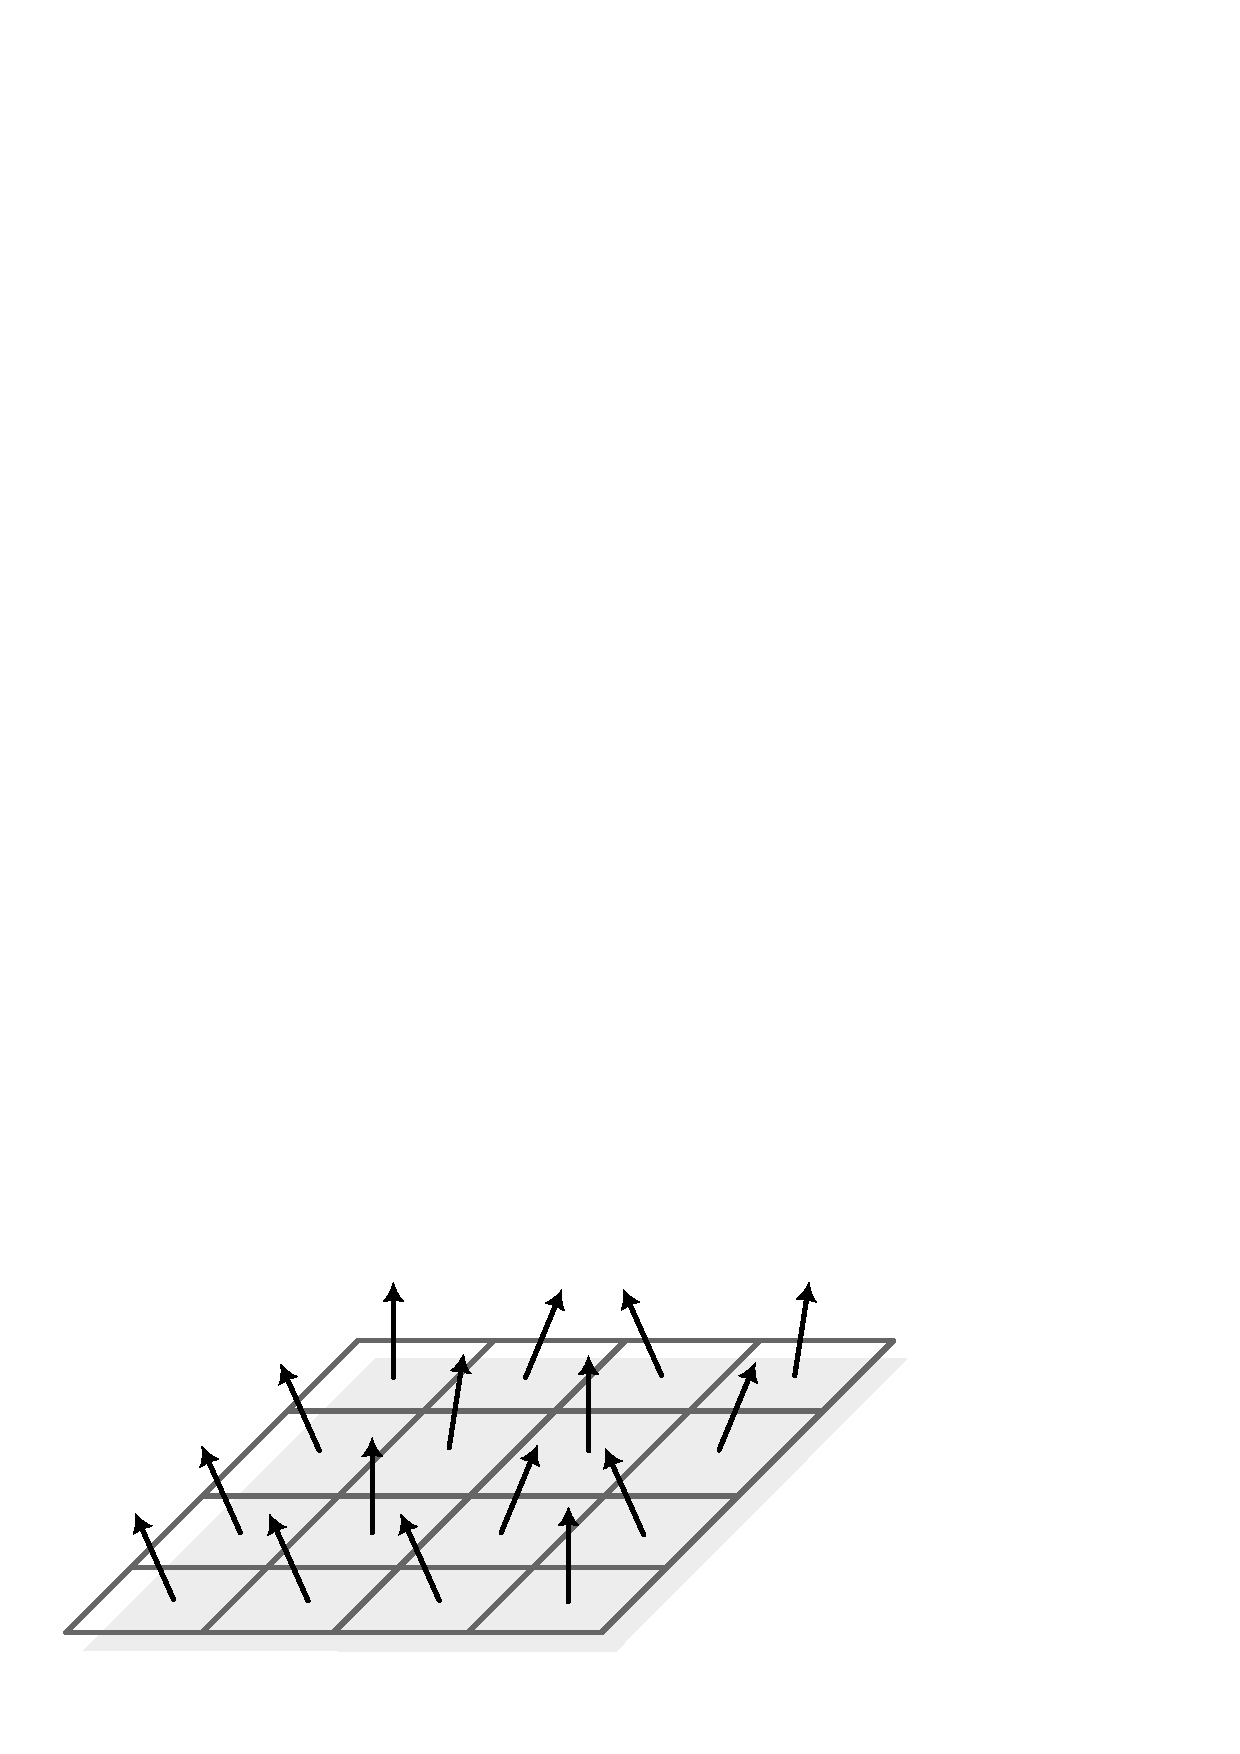
\includegraphics[width=0.75\columnwidth]{ml-figures/som/som-diagram.pdf}
  \caption{A Self Organizing Map with nodes configured in a rectangular grid topology with weight vectors randomly initialized.}
  \label{fig:som-diagram}
\end{figure}
One can initialize the weights in a variety of ways. Some common choices are
\begin{itemize}
\item Randomly initialize them as in figure \ref{fig:som-diagram}.
\item Initialize them to the value of $n$-many randomly selected data samples $\mathbf{x}_i$.
\item Initilize them to the first $n$-many principal components of the dataset.
\end{itemize}

Next, we proceed to update the weights according to the following steps for each $\mathbf{x}_k$ datum:
\begin{enumerate}
\item Compute the \textit{best match unit} (BMU) as
  \begin{equation}
    \mathbf{w}_{i}^{\text{best}} = \text{arg}\min\limits_{\mathbf{w}_j} \left( d(\mathbf{x}_k, \mathbf{w}_j)^2 \right)
  \end{equation}
  where $d(\cdot,\cdot)$ is some suitably chosen distance function. One often defaults to the Euclidean metric.
\item Choose a radius $\sigma_t$ which we will use to identify the correct update for to apply to all nodes relative to $\mathbf{w}_i^{\text{best}}$.
\item Update \textit{all} the weights according to the equation
  \begin{equation}
    w_{m}^{t+1} = w_m^{t} + \eta(t)f(x_m,y_n,\sigma_t)\left(\mathbf{x}_k  - \mathbf{w}_n^{t} \right)
  \end{equation}
  where $\eta(t)$ is the learning rate, and $f(x_m, y_m, \sigma_t)$ is the \textit{neighborhood} function which defines the relative amount each node $\mathbf{w}_m$ is updated according to its coordinate distance from the best match unit (i.e. the distance between the points $(x_m, y_m)$ and $(x_{\text{best}}, y_{\text{best}})$ in the two dimensional case). Typically one chooses a the learning rate to evolve according to the schedule
  \begin{equation}
    \eta(t) = \eta_0\exp(^-\lambda t)
  \end{equation}
  with the radius $\sigma_t$ evolving similarly according to
  \begin{equation}
    \sigma_t = \sigma_0\exp(-\beta t).
  \end{equation}
  Popular choices for the neighborhood function are the Gaussian function, Mexican-hat function, a cone function, and a cylinder function.
\end{enumerate}

\subsubsection{A simple example: partitioning color spaces}

As an illustrative example, consider the minimal dataset formed by the colors red, green, and blue which as vectors may be written as
\begin{align}
  \text{Red} &= \left(1,\; 0,\; 0 \right)\\
  \text{Green} &= \left(0,\; 1,\; 0 \right) \\
  \text{Blue} &= \left(0,\; 0,\; 1 \right).
\end{align}
Now let us suppose we want to train an SOM to generate a classification for colors using only these three as the supplied training data. Figure \ref{fig:som-demo} shows exactly this. Here we have trained an SOM of size $25 \times 25$ cells in a flat hexagonal topology. As the weight vectors are themselves vectors of length $3$, we can then visualize the trained SOM by coloring each corresponding node by the color learned in its weight vector. What we find is that the resulting map has clearly separated red, green, and blue into distinct regions in the grid, and more importantly, there is a smooth gradient between neighboring cells reflecting the fact that neighboring classes are more \textit{similar} than cells with a large separation distance. This is not the case for many other common clustering techniques like k-nearest neighbors or DBSCAN for which relationship between learned classes is challenging to interpret.

\begin{figure}[h!]
  \centering
  \includegraphics[width=0.75\columnwidth]{ml-figures/som/SOM_demo.pdf}
  \caption{A trained Self Organizing Map of $25\times 25$ cells in a hexagonal topology trained on a dataset consisting of the three colors red, green, and blue.}
  \label{fig:som-demo}
\end{figure}

To enable this demonstration and its subsequent use throughout the rest of this dissertation, I have created a new open-source implementation of the SOM algorithm for the Julia programming language called \texttt{SelfOrganizingMaps.jl} which has been added to the general registry and can by freely downloaded for use by anyone. The repository for the code as well as the associated documentation can be found at \href{https://github.com/john-waczak/SelfOrganizingMaps.jl}{this site}.

\subsection{Generative Topographic Maps}

Now that we've developed the SOM algorithm, we see upon reflection that there are a few drawbacks to the methods, namely
\begin{itemize}
\item There is no probabilistic interpretation of the fitted SOM? Are we to trust the fit results with $100\%$ certainty?
\item There is no clearly stopping criteria for the learning process? How many epochs should be performed? Do you simply stop the training once the neighbor radius $\sigma_t$ is less than the minimum neighbor distance?
\end{itemize}
With this in mind, we now seek to introduce a new method based on the SOM which will allow us to address the shortcomings by taking a principled, probabilistic approach, which will be called the \textit{Generative Topographic Mapping} (GTM). This technique was first introduced by Bishop et al. in  \cite{gtm-orig} and our derivation of the method will follow their presentation closely.

Both the SOM and GTM rely on the assumption that our high dimensional dataset $\D\subseteq\R^D$ can be accurately represented as being constrained to a lower dimensional submanifold. In the SOM this is acheived by assigning coordinates to each of the weight vectors according to some predetermined grid. In the GTM, however, we make a slight change in our perspective and say that the high dimensional data we have are \textit{generated} from some lower dimensional set of \textit{latent vectors} living in $\R^L$ with $L < D$. For ease of visualization, it is standard to chose $L=2$. Our goal, then, is to learn a mapping from the latent space to the data space which \textit{maximizes the likelihood} of obtaining our dataset given the set of latent variables.

In the coming derivation, we shall assume the following notations:
\begin{equation}
  \begin{aligned}
    \mathbf{x}\in\R^L &\quad \text{The latent vector} \\
    \mathbf{t}_n\in\R^D &\quad \text{The data vector(s) }n=1,...,D \\
    \mathbf{y}=\mathbf{y}(\mathbf{x};W) &\quad \text{The transformation } \mathbf{y}:\R^L\to\R^D
    W &\quad \text{The model weights}
  \end{aligned}
\end{equation}


%------------------------------------------------------------------------------------------%

\section{Dimensionality Redution}
\subsection{PCA}
\subsection{ICA}
\subsection{t-SNE}


%------------------------------------------------------------------------------------------%

\section{Model Ensembling}
MLJ and SciKitLearn documentation sites will have good references for this, I think.
\subsection{Bagging}
e.g. Random Forests
\subsection{Boosting}
e.g. XGBoost
\subsection{Stacking}
e.g. Super Learners. Use the example of model stacking from MLJ documentation to describe our approach.



%------------------------------------------------------------------------------------------%

\section{Uncertainty Quantification}
The focus of this section can be on the concept of uncertainty quantification. For many physics theories that are nicely linearized, uncertainty analysis can be easily accomplished at the level of first order sensitivites. That is, we can look at the Jacobian of our model to infer the behavior of small deviations about initial conditions. This approach does not easily extend to more complicated domains where the nonlinear effects dominate. Further, we also often want to establish ways to think about the fundamental instrument uncertainty for a measuring device. This can require meticulous calibrations which often assume a linear or polynomial fit... We can do better. Why not let the data tell us what the measurement uncertainty really is?

A good motivating example for the discussion of instrumental uncertainty is the use of a thermistor to measure temperature. One must assume a reasonable range of temperatures to establish the linear relationship between temperature and resistivity that is used determine the temperature. However, the material characteristics of the thermistor that introduce nonlinearities at extreme temperatures don't necessarily mean we should have to throw out measurements that do not fall within this well-behaved range. Rather, we can preform a more sophisticated *calibration* to learn a model mapping resistivity to temperature that can account for these effects.

This is the bread-and-butter of the MINTS sensing efforts. Often low-cost sensing solutions provide decent measurements within a limit domain. With quality data from superior (but often prohibitively expensive) reference instruments, we can improve the default calibration to improve the reliability of data (by reducing uncertainty) and extend it's domain of usefulness.

\subsection{Quantile Regression}
\subsection{Probabilistic Models}
e.g. discuss models like the GPR which fundamentally produce \textit{distributions}. Similarly for models like Neural Networks that can produce multiple outputs, we can train a model to predict both $\mu$ and $\sigma$ to make the model probabilistic.

\subsection{Conformal Prediction}



%------------------------------------------------------------------------------------------%

\section{Scientific Machine Learning}
\subsection{Physics-Informed Neural Networks}
\subsection{Universal Differential Equations}
\subsection{Adjoint Methods for ODEs: Neural Ordinary Differential Equations}
\subsection{Hamiltonian Neural Networks}



%------------------------------------------------------------------------------------------%

%% \section{Generative Methods}
%% \subsection{Auto Encoders}
%% \subsection{Generative Adversarial Networks}


%------------------------------------------------------------------------------------------%

\section{Data Assimilation}

\textcolor{red}{NOTE: We should add further derivations from a Bayesian framework to fit in with what we've done for the Gaussian process regression and generative topographic maps. We should also add some more generic background to the topic of Data Assimilation, it's first uses in Meteorology, }


The proper application of scientific models to make real-world predictions requires that we commit ourselves to a full accounting of all possible sources of uncertainty when reporting results. Further, the explosion of \textit{big data} across scientific fields provieds a plethora observational data that our models are typically unequipped to incorporate when making predictions. The field of \textit{Data Assimilation} addresses this problem by providing a family of techniques engineered to combine model output together with observational data whilst enabling a complete accounting the sources of uncertainty. For chaotic systems in particular, data assimilation enables integration on long time scales that would be impossible via models alone. In this overview, we will follow the examples from \cite{pyda}.

Data assimilation can be cleanly developed in the framework of discrete dynamical systems. Since, at the end of the day, all of our scientific models must be discretized to be evaluated numerically, this is a reasonable course of action. Our goal is to find the best prediction for the system state vector $u$ that combines our model predictions, also known as \textit{forecasts}, with observational data. Model predictions are described via the discrete update equation:
\begin{equation}
    u_{k+1} = \mathcal{M}(u_k; \theta)
\end{equation}
For ODE systems, $\mathcal{M}$ represents the time integration scheme for a models like
\begin{equation}
    \dfrac{du}{dt} = f(u, t; \theta),
\end{equation}
in other words, a particular choice of ODE integration scheme (Runge Kutta for example) used to evolve the state vector $\u$ from time $u_k$ to $u_{k+1}$.

To measure the performance of our assimilation scheme, we denote the \textit{true} value of the state vector as $u^{(t)}$. The output of our model is denoted $u^{(b)}$ (\textit{b} superscript for \textit{background}). The discrepancy between the true value and our forecast is denoted $\xi^{(b)} = u^{(t)} - u^{(b)}$ characterizing the extent to which our model prediction is imperfect. The observations of our system are denoted by $w_k = w(t_k)$. These observations do not necessarily need to be components of the state vector $u$, but rather, are related to it via the \textit{observation function}, $h:u_k\mapsto w_k$. For example, one may attempt to predict surface sea temperatures using data assimilation with data from satellite observations. The function $h$ would then be the Stefan-Boltzmann relating the measured spectra to temperature. However, real world data is \textit{also} imperfect, which we must take into account let we over constrain our model with poor quality data. We write
\begin{equation}
    w_k = h(u_k) + \xi_k^{(m)}
\end{equation}
where $\xi_k^{(m)}$ denotes this measurement error.

Given our model predictions $u_{k}^{(b)}$ and observations $w_k$, we seek to obtain the \textit{optimal} or best-possible prediction called the \textbf{analysis}, $u^{(a)}$. Despite our care, this analysis will still be imperfect, so we further define the analysis error as
\begin{equation}
\xi^{(a)} = u^{(t)} - u^{(a)}
\end{equation}

In summary, we have defined the following relevant quantities (at time $t_k$):
\begin{align}
  &u_k^{(t)} \in \mathbb{R}^n &\text{the true state vector} \\
  &u_k^{(b)} \in \mathbb{R}^n &\text{the model forecast} \\
  &u_k^{(a)} \in \mathbb{R}^n &\text{the analysis} \\
  &w_k \in \mathbb{R}^m &\text{the observation vector} \\
  &\xi^{(b)} \in \mathbb{R}^n &\text{the model forecast error}\\
  &\xi^{(m)} \in \mathbb{R}^m &\text{the observation noise vector}\\
  &\xi^{(a)} \in \mathbb{R}^n &\text{the analysis error}\\
  &\xi^{(p)} \in \mathbb{R}^n &\text{the process noise if we used our model on the true state}\\
  &\mathcal{M}:\mathbb{R}^n\to\mathbb{R}^n &\text{the discrete model evolution function}\\
  &f:\mathbb{R}^n\to\mathbb{R}^n &\text{differential equation model (the right hand side)}\\
  &h:\mathbb{R}^n\to\mathbb{R}^m  &\text{observation function}
\end{align}

To move forward, we now establish the following (prior) assumptions about the distribution of errors in each component in order to make it possible to derive a closed form for the final analysis. We require
\begin{align}
  &\E[\xi_k^{(b)}] = 0 & &\E[\xi_k^{(b)}(\xi_j^{(b)})^T] = 0 \text{ for } k\neq j\\
  &\E[\xi_k^{(m)}] = 0 & &\E[\xi_k^{(m)}(\xi_j^{(m)})^T] = 0 \text{ for } k\neq j\\
  &\E[\xi_k^{(b)}(u_0)^T] = 0 & &\E[\xi_k^{(m)}(u_0)^T] = 0\\
  &\E[\xi_k^{(b)}\xi_j^{(m)}] = 0 & &  % \\
  %% &\E[u_k^{(t)}] = u_k^{(b)} & &
\end{align}
or in words, the errors in our model and observation are unbiased (e.g. mean zero) and uncorrelated.

We also define the error covariance matrices
\begin{align}
  Q_k &:= \E[\xi_k^{(p)}(\xi_k^{(p)})^T] \\
  R_k &:= \E[\xi_k^{(m)}(\xi_k^{(m)})^T] \\
  B_k &:= \E[\xi_k^{(b)}(\xi_k^{(b)})^T]
\end{align}
which we will use in our consideration of the final error of our analysis.

\subsection{Kalman Filter}
Given some model for the error covariance matrices $Q_k$ and $R_k$, we would like a method that propagates \textit{both} our model \emph{and} the errors forward. This way we may guarantee that the accuracy of our analysis doesn't come at the cost of higher uncertainty.

The original implementation of the Kalman filter was for strictly linear systems, in particular as a filter for signal processing. We will first develop the analysis for this simplified case adn then will generalize to the \textit{Extended Kalman Filter} (EKF) that can handle fully nonlinear situations.

In the linear case, our system may be written as
\begin{align}
    u_{k+1}^{(t)} &= M_ku_k^{(t)} + \xi_{k+1}^{(p)} \\
    w_k &= H_ku_k^{(t)} + \xi_k^{(m)}
\end{align}
where $M_k$ and $H_k$ are now matrices defining the linear problem.

The goal of the Kalman filter is to derive the analysis $u^{(a)}$ which minimizes the trace of the analysis error covariance matrix (i.e. sum of squared errors): \begin{equation}
    \mathrm{Tr}\left( P_k\right) := \E[(u_k^{(t)}-u_k^{(a)})^T(u_k^{(t)}-u_k^{(a)})]
\end{equation}
Finding the analysis consists of two steps: the forecast step and the assimilation step.

Beginning with the forecasting step, assume we have the analysis at time $t_k$ denoted $u_k^{(a)}$. Then the forecast for time $t_{k+1}$ is
\begin{equation}
    u_{k+1}^{(b)} = M_ku_k^{(a)},
\end{equation}
or in words, we obtain the next prediction by evolving the previous analysis forward. The background error is therefore
\begin{align}
    \xi_{k+1}^{(b)} &= u_{k+1}^{(t)} - u_{k+1}^{(b)} \\
    &= M_ku_k^{(t)}+\xi_{k+1}^{(p)} - M_{k}u_k^{(a)} \\
    &= M_k\left(u_k^{(t)}-u_k^{(a)} \right) + \xi_{k+1}^{(p)} \\
    &= M_k\xi_k^{(a)} + \xi_{k+1}^{(p)}
\end{align}

We may now evaluate the covariance matrix of our background estimate as:
\begin{align}
    B_{k+1} &= \E[\xi_{k+1}^{(b)}(\xi_{k+1}^{(b)})^T] \\
    &= \E\left[\left(M_k\xi_k^{(a)} + \xi_{k+1}^p \right) \left(M_k\xi_k^{(a)} + \xi_{k+1}^p \right)^T \right] \\
\end{align}

If we presume that $\E[\xi_k^{(b)}(\xi_{k+1}^{(p)})^T] = 0$, then the cross terms vanish and we are left with
\begin{equation}
    \boxed{B_{k+1} = M_kP_kM_k^T + Q_{k+1}}
\end{equation}

Thus we now have the background (i.e forecast) estimate of the state at $t_{k+1}$ and its covariance matrix. Given a measurement $w_{k+1}$ at the same time with covariance matrix $R_{k+1}$, we may now perform the assimilation step where we fuse the two sources of information to obtain $u_{k+1}^{(a)}$ and $P_{k+1}$.

Let's suppose that the analysis has the form
\begin{equation}
    u_{k+1}^{(a)} = \nu + K_{k+1}w_{k+1}
\end{equation}

for some vector $\nu\in\R^n$ and matrix $K_{k+1}\in\R^{m\times n}$. In a perfect world, we would have $\E[u_{k}^{(t)}-u_{k}^{(a)}] = 0$. Therefore,

\begin{align}
    0 &= \E[u_k^{(t)} - u_k^{(a)}] \\
    &= \E[(u_k^{(b)} + \xi_k^{(b)}) - (\nu + K_kw_k)] \\
    &= \E[(u_k^{(b)} + \xi_k^{(b)}) - (\nu + K_kH_ku_k^{(t)} + K_k\xi_k^{(m)})] \\
    &= \E[u_k^{(b)}] + \E[\xi_k^{(b)}] - \E[\nu] -K_kH_k\E[u_k^{(t)}] - K_k\E[\xi_k^{(m)}]\\
    &= u_k^{(b)} + 0 - \nu - K_kH_ku_k^{(b)} - 0 \\
    &= u_k^{(b)} - \nu - K_kH_ku_k^{(b)} \\
    \Rightarrow \nu &= u_k^{(b)} - K_kH_ku_k^{(b)}
\end{align}

which we now substitute to obtain

\begin{equation}
    \boxed{u_k^{(a)} = u_k^{(b)} + K_k(w_k - H_ku_k^{(b)})}
\end{equation}

Now that we know the form for the analysis we may derive the optimal matrix $K_k$ by optimization of $P_k$. We have

\begin{align}
	\xi_k^{(a)} &= u_k^{(t)} - u_k^{(a)} \\
                &= M_{k-1}u_{k-1}^{(t)} + \xi_{k}^{(p)} - u_k^{(b)} - K_k\left(w_k - H_ku_k^{(b)} \right) \\
                &= M_{k-1}u_{k-1}^{(t)} + \xi_{k}^{(p)} - M_{k-1}u_{k-1}^{(a)} - K_k\left(H_ku_k^{(t)} + \xi_k^{(m)} - H_ku_k^{(b)} \right) \\
                &= M_{k-1}u_{k-1}^{(t)} + \xi_{k}^{(p)} - M_{k-1}u_{k-1}^{(a)} - K_kH_ku_k^{(t)} - K_k\xi_k^{(m)} + K_kH_ku_k^{(b)} \\
                &= M_{k-1}u_{k-1}^{(t)} + \xi_{k}^{(p)} - M_{k-1}u_{k-1}^{(a)} - K_kH_ku_k^{(t)} - K_k\xi_k^{(m)} + K_kH_ku_k^{(b)} \\
                &= \Big\{ M_{k-1}(\xi_{k-1}^{(a)}+u_{k-1}^{(a)}) + \xi_{k}^{(p)} - M_{k-1}u_{k-1}^{(a)} \Big\} - K_kH_ku_k^{(t)} - K_k\xi_k^{(m)} + K_kH_ku_k^{(b)} \\
                &= \Big\{ M_{k-1}\xi_{k-1}^{(a)} + \xi_{k}^{(p)} \Big\} - K_kH_ku_k^{(t)} + K_kH_ku_k^{(b)} - K_k\xi_k^{(m)}\\
                &= M_{k-1}\xi_{k-1}^{(a)} + \xi_{k}^{(p)} - K_kH_k(M_{k-1}u_{k-1}^{(t)} + \xi_k^{(b)}) + K_kH_ku_k^{(b)} - K_k\xi_k^{(m)}\\
                &= M_{k-1}\xi_{k-1}^{(a)} + \xi_{k}^{(p)} - K_kH_kM_{k-1}(\xi_{k-1}^{(a)} + u_{k-1}^a) - K_kH_k\xi_k^{(b)} + K_kH_ku_k^{(b)} - K_k\xi_k^{(m)}\\
                &= M_{k-1}\xi_{k-1}^{(a)} + \xi_{k}^{(p)} - K_kH_kM_{k-1}(\xi_{k-1}^{(a)} + u_{k-1}^a) - K_kH_k\xi_k^{(b)} + K_kH_kM_{k-1}u_{k-1}^{(a)} - K_k\xi_k^{(m)}\\
                &= M_{k-1}\xi_{k-1}^{(a)} + \xi_{k}^{(p)} - K_kH_kM_{k-1}\xi_{k-1}^{(a)} - K_kH_k\xi_k^{(b)} - K_k\xi_k^{(m)}\\
                &= \big(I-K_kH_k \big)(M_{k-1}\xi_{k-1}^{(a)} - \xi_{k}^p) - K_k\xi_k^{(m)}\\
\end{align}

and therefore the covariance matrix is

\begin{align}
    P_k &= \E[\xi_{k}^{(a)}(\xi_{k}^{(a)})^T] \\
        &= \E\Big[\left(\big(I-K_kH_k \big)(M_{k-1}\xi_{k-1}^{(a)} - \xi_{k}^p) - K_k\xi_k^{(m)} \right) \left(\big(I-K_kH_k \big)(M_{k-1}\xi_{k-1}^{(a)} - \xi_{k}^p) - K_k\xi_k^{(m)} \right)^T \Big] \\
        &= \big(I-K_kH_k \big)M_{k-1}\E[\xi_{k-1}^{(a)}(\xi_{k-1}^{(a)})^T]M_{k-1}^T\big(I-K_kH_k \big)^T \\
        &\qquad \qquad + \big(I-K_kH_k \big)\E[\xi_k^{(p)}(\xi_k^{(p)})^T]\big(I-K_kH_k \big)^T \notag\\
        & \qquad \qquad - K_k\E[\xi_{k}^{(m)}(\xi_k^{(m)})^T]K_k^T \notag\\
        &= \big(I-K_kH_k \big)B_k\big(I-K_kH_k \big)^T - K_kR_kK_k^T
\end{align}

Now all that remains is to derive the specific form for $K_k$. The Kalman filter is defined as that $K_k$ which which minimizes the sum of squared analysis errors, i.e. the trace of the analysis error covariance matrix. Therefore, the following identities from matrix calculus will be useful:
\begin{align}
    \mathop{\nabla}_{A}\text{tr}(AB) &= B^T \\
    \mathop{\nabla}_{A}\text{tr}(BA^T) &= B \\
    \mathop{\nabla}_{A}\text{tr}(ABA^T) &= AB^T + AB  \\
\end{align}
from which we obtain
\begin{align}
    0 &= \mathop{\nabla}_{K_k}\text{tr}(P_k) \\
      &= \mathop{\nabla}_{K_k}\Big\{ B_k -B_kH_k^TK_k^T - K_kH_kB_k  + K_kH_kB_kH_k^TB_k^T - K_kR_kK_k^T \Big\} \\
      &= -B_kH_k^T - (H_kB_k)^T + K_k\left[H_kB_kH_k^T + (H_kB_kH_k^T)^T - R_k+R_k^T\right] \\
      &= -2B_kH_k^T + 2K_k\left(H_kB_kH_k^2 - R_k \right) \\
  \Rightarrow K_k &= B_kH_k^T\Big[ H_kB_kH_k^T - R_k \Big]^{-1}
\end{align}
we now substitute this result to obtain a simplified form for $P_k$:
\begin{align}
    P_k &= \left(I - K_kH_k \right)B_k\left(I - K_kH_k \right)^T + K_kR_kK_k^T \\
        &= \left(I - K_kH_k \right)B_k - \left(I - K_kH_k \right)B_k\left(K_kH_k \right)^T + K_kR_kK_k^T \\
        &= \left(I - K_kH_k \right)B_k -\left\{ \left(I - K_kH_k \right)B_k\left(K_kH_k \right)^T + K_kR_kK_k^T \right\} \\
        &= \left(I - K_kH_k \right)B_k -\left\{ \left(I - K_kH_k \right)B_kH_k^TK_k^T + K_kR_kK_k^T \right\} \\
        &= \left(I - K_kH_k \right)B_k -\left\{ \left(I - K_kH_k \right)B_kH_k^T + K_kR_k \right\}K_k^T \\
        &= \left(I - K_kH_k \right)B_k -\left\{ B_kH_k^T - K_k\left( H_kB_kH_k^T + R_k \right)  \right\}K_k^T \\
        &= \left(I - K_kH_k \right)B_k -\left\{ B_kH_k^T - B_kH_k^T \right\}K_k^T \\
        &= \left(I - K_kH_k \right)B_k
\end{align}
where we have used the fact that covariance matrices are symmetric.


Now that we have all of the pieces, let's summarize the procedure:
\begin{enumerate}
\item \textbf{Initialization}: We must set the system to some initial condition. This means we must define $u_0^a$ and $P_0$. We must also come up with a model for the process noise covariance $Q_k$ and measurement error covariance $R_k$.
\item \textbf{Forecast Step}: Starting with the analysis state vector $u^{(a)}_{k-1}$ and covariance $P_{k-1}$, we apply the model time evolution operator $M_{k-1}$ to obtain the predicted state $u^{(b)}_{k}$ and covariance $B_k$ at the next time step.
  \begin{align}
    u_k^{(b)} &= M_{k-1}u_{k-1}^{(a)} \\
    B_k &= M_{k-1}P_{k-1}M_{k-1}^T + Q_{k}
  \end{align}
\item \textbf{Assimilation Step}: Combine our observations $w_k$ and their associated uncertainties contained in $R_k$ together with the background prediction $u^{(b)}_k$ and it's error covariance matrix $B_k$ to obtain the analysis state $u^{(a)}_k$ and error covariance $P_k$.
  \begin{align}
    K_k &= B_kH_k^T\Big[ H_kB_kH_k^T - R_k \Big]^{-1}  \\
    u_k^{(a)} &= u_k^{(b)} + K_k(w_k - H_ku_k^{(b)})\\
    P_k &= \left(I - K_kH_k \right)B_k
  \end{align}
\end{enumerate}


\subsection{Extended Kalman Filter}

Given the nonlinear nature of many scientific models, it is desirable to extend out notion of the \textit{Kalman Filter} to be able to handle nonlinear models $f(\cdot)$ (and by extension, their update function $\mathcal{M}(\cdot)$), and nonlinear observation functions $h(\cdot)$. This can be accomplished so long as these functions are sufficiently smooth ($C^1$ to be precise) so as to admit valid Taylor approximations to first order. That is,
\begin{align}
    \mathcal{M}(u_{k}) &\approx \mathcal{M}(u_k^{(a)}) + D_{M}(u_k^{(a)})\xi_k^{(a)} & h(u_k) &\approx h(u_k^{(b)}) + D_h(u_k^{(b)})\xi_k^{(b)} \\
    D_{M} &:= \left[\dfrac{\partial \mathcal{M}_i}{\partial u_j} \right] & D_h &:= \left[ \dfrac{\partial h_i}{\partial u_j}\right]
\end{align}
where $\mathcal{M}_i$ and $h_i$  denote the ith component functions of $\mathcal{M}$ and $h$ respectively. For the so-called \textit{Extended Kalman Filter} (EKF), approach. We assume that the analysis errors can be reasonably approximated to evolve linearly such that we can use the above \textit{linearized} approximations to our model update and observation functions to reasonably model our uncertainties.

We therefore replace the (previously) linear functions $M_k$ and $H_k$ with their nonlinear Jacobian derived counterparts to obtain the following procedure
\begin{enumerate}
\item \textbf{Initialization}: To begin we must choose values for $u_0^{(a)}$ and $P_0$. We must also provide models for $Q_k$ and $R_k$.
\item \textbf{Forecast Step}:
\begin{align}
    u_k^{(b)} &= \mathcal{M}(u_{k-1}^{(a)}) \\
    B_k &= D_M(u_{k-1}^{(a)})P_{k-1}D_M^T(u_{k-1}^{(a)}) + Q_k
\end{align}
\item \textbf{Assimilation Step}:
\begin{align}
    K_k &= B_kD_h^T(u_k^{(b)})\left[ D_h(u_k^{(b)})B_kD_h^T(u_k^{(b)}) + R_k \right]^{-1}\\
    u_k^{(a)} &= u_k^{(b)} + K_k(w_k - h(u_k^{(b)})) \\
    P_k &= \left( I - K_kD_h(u_k^{(b)}) \right)B_k
\end{align}
\end{enumerate}
Note that the most challenging piece in this implementation is to stably compute the model update Jacobian $D_M$, as this is not just the Jacobian of our continuous model $f(\cdot)$. For example, if we are modeling the state of the system via a set of ODEs, then $D_M$ is the Jacobian of the output of a single integrator step with respect to the initial starting state. This can pose significant computational challenges where adaptive solvers are desired as we must be able to back-propagate out derivative information for all evaluations of the function $f(\cdot)$ taken during the step.


\subsection{continuous-discrete Extended Kalman Filter}

So far in our discussion of data assimilation techniques we have limited ourselves to discretized realizations of continuous models and measurements. This allowed us to derive reasonable update equations for the error covariance matrix and analysis by considering the changes that occur by application of our model evolution operator $\mathcal{M}$. In practice though the case tends to be slightly different: the underlying dynamics are understood to evolve continuously despite our access to finite time measurements at some frequency. For this reason, it would be preferable to utilize our knowledge of the model covariance $Q$ together with the continuous dynamics of the model itself to allow the background covariance matrix to evolve continuously between measurements. Then, only when we have access to new data to we need to perform a discrete update by computing the Kalman gain and generating a new analysis as before. As we shall see, this strategy yields an augmented dynamical system for which
\begin{equation}
  \begin{cases}
    \dfrac{du}{dt} = f(u,t;\theta) + \xi^{(b)}(t) \\
    \dfrac{P}{dt} = J_{u}(t)P(t) + P(t)J_{u}^T(t) + Q(t)
  \end{cases}
\end{equation}
where $J_{u}=\frac{\partial f}{\partial u}$ is the Jacobian of the system with respect to the state vector $u$. To derive this new form for the Extended Kalman filter, let us first begin with a linear system for which \textit{both} the underlying dynamics continuously, that is
\begin{equation}
  \begin{cases}
    \dot{u} = Mu + \xi^{(b)} \\
    w_k = Hu_k + \xi^{(m)}_k
  \end{cases}
\end{equation}
where $\xi^{(b)}$ now represents a Weiner process (e.g. Gaussian white noise process) of covariance $Q(t)$. Presuming the model covariance is still uncorrelated with the measurement means that we now have:
\begin{align}
  \E[\xi^{(b)}(t)(\xi^{(b)}(\tau))^T] &= Q(t)\delta (t-\tau) \\
  \E[\xi^{(m)}(\xi^{(b)}(t))^T] &= 0
\end{align}

To move forward, we now need to establish the relationship between our previous $Q_k$ and $Q$ so that in the limit as $\Delta t\to 0$, we may obtain the new dynamical equations. If we understand $Q_k$ to be the model error \textit{accumulated} over the integration window, then it follows that
\begin{equation}
  \begin{aligned}
    Q_k &\approx \int \int d\zeta d\eta \E[\xi^{(b)}(\zeta)(\xi^{(b)}(\eta))^T] \\
    &= \int \int d\zeta d\eta Q(\zeta)\delta(\zeta - \eta) \\
    &= \int\limits_{t_{k-1}}^{t_k}Q(\zeta)d\zeta \\
    &\approx Q(t_k)\Delta t
  \end{aligned}
\end{equation}
This tells us all that we need! For small enough $\Delta t$, we may approximate our continuous dynamics by
\begin{equation}
  \frac{u_{k+1}-u_{k}}{\Delta t} = Mu_k + \xi^{(b)}_k
\end{equation}
and therefore
\begin{equation}
  u_{k+1} = (I-\Delta t M)u_{k} + \xi^{(b)}_k
\end{equation}
from which we can identify our linear $M_k$ matrix from the original discrete Kalman filter as $(I+\Delta t M)$ in the discretized version of this new continuous model. Substituting this in to our expression for the forecast step yields
\begin{equation}
  B_{k+1} = \left(I + \Delta t M \right)P_k\left(I + \Delta t M \right)^T + Q\Delta t.
\end{equation}
Expanding this expression and keeping only terms of $\mathcal{O}(\Delta t)$, we find
\begin{equation}
  \begin{aligned}
  B_{k+1} &= P_k + \Delta t MP_k + P_kM^T\Delta t + MP_kM^T\Delta t^2 + Q\Delta t \\
  &\approx P_k + \Delta t M P_k + \Delta t P_k M^T + Q\Delta t
  \end{aligned}
\end{equation}
As we shrink $\Delta t$ to zero between observations, there is no longer a distinction between the background covariance $B_k$ and the analysis covariance $P_k$ so that we may write rearrange and take the limit
\begin{equation}
  \lim_{\Delta t \to 0}\frac{P_{k+1}-P_k}{\Delta t} = \lim_{\Delta t \to 0} MP_k + P_kM^T + Q
\end{equation}
which evaluates to
\begin{equation}
  \boxed{\frac{d}{dt}P = MP(t) + P(t)M^T + Q(t)}
\end{equation}

To \textit{extend} this linear version to the case of nonlinear model and observation functions, we linearize our nonlinear model so that $M\mapsto J_{u}=\partial f/\partial u$. This then leads to the continuous-discrete Extended Kalman Filter for which the procedure is as follows
\begin{enumerate}
\item \textbf{Initialization}: To begin we choose initial values for $u_0^{(a)}$ and $P_0$. We must also provide initial covariance values $R_0$ and $Q(0)$.
\item \textbf{Forecast Step}: Integrate the dynamical system
  \begin{equation}
    \begin{cases}
      \dfrac{du}{dt} = f(u,t;\theta) \\
      \dfrac{dP}{dt} = J_{u}P(t) + P(t)J_{u}^T + Q(t)
    \end{cases}
  \end{equation}
  from $t_{k-1}$ to $t_{k}$ to obtain $u_{k}$ and $P_{k}$
\item \textbf{Assimilation Step}: Compute the Kalman gain and update the state vector and associated covariance matrix according to
  \begin{align}
    K_k &= P_kD_{h}^T(u_k)\left[ D_h(u_k)P_kD_h^T(u_k) + R_k \right]^{-1} \\
    u_k &\mapsto u_k + K_k(w_k - h(u_k)) \\
    P_k &\mapsto (I - K_kD_h(u_k))P_k
  \end{align}
\end{enumerate}




\subsection{3d-Var}

For the \textit{Kalman Filter} and the \textit{EKF}, we derived an optimal way to combine observation with simulation so as to minimize the trace of the analysis error covariance matrix, $P_k$. An alternative approach is to recast the problem as a pure optimzation problem where rather than finding a filter $K_k$ that will add an innovation to $u_k^{(b)}$ to obtain the analysis $u_k^{(a)}$, we obtain the analysis by directly optimizing a cost function
\begin{equation}
J(u) = \frac{1}{2}\left(w - h(u) \right)^TR^{-1}\left(w - h(u) \right) + \frac{1}{2}\left(u - u^{(b)} \right)^TB^{-1}\frac{1}{2}\left(u - u^{(b)} \right)
\end{equation}
which we can justify as coming from the joint probability distribution (assuming Gaussian errors)
\begin{equation}
\mathcal{P}(u|w) = C\exp\left(- \frac{1}{2}\left(u - u^{(b)} \right)^TB^{-1}\frac{1}{2}\left(u - u^{(b)} \right) \right)\cdot\exp\left(-  \frac{1}{2}\left(w - h(u) \right)^TR^{-1}\left(w - h(u) \right) \right)
\end{equation}
with model error covariance $B$ and measurement error covariance $R$ as before. This is clearly a \textit{very strong assumption}.

To optimize $J(u)$, we begin by taking it's gradient.
\begin{equation}
    \nabla_uJ(u) = -D_h^TR^{-1}(w-h(u)) + B^{-1}(u-u^{(b)})
\end{equation}
Thus, finding the analysis $u^{(a)}$ ammounts to solving the system
\begin{equation}
    a-D_h^TR^{-1}(w-h(u^{(a)})) + B^{-1}(u^{(a)}-u^{(b)}) = 0
\end{equation}

As for Kalman filtering, let's begin with the assumption that our model and observation function are linear. Suppose that we have $h(u) = Hu$ so that $D_h(u) = H$. It follows that
\begin{align}
  D_h^TR^{-1}(w-Hu^{(a)}) &= B^{-1}(u^{(a)}-u^{(b)}) \\
  D_h^TR^{-1}w - D_h^TR^{-1}Hu^{(a)} &= B^{-1}u^{(a)} - B^{-1}u^{(b)} \\
  \left(D_h^TR^{-1}H + B^{-1} \right)u^{(a)} &= D_h^TR^{-1} + B^{-1}u^{(b)} \\
  \left(H^TR^{-1}H + B^{-1} \right)u^{(a)} &= H^TR^{-1} + B^{-1}u^{(b)}
\end{align}

Thus we see that the analysis is given by
\begin{equation}
  u^{(a)} = u^{(b)} + BH^T\left( R + HB^TH \right)^{-1}(w-Hu^{(b)})
\end{equation}
which agrees with what we found for the Linear Kalman Filter.


Moving on to the non-linear case, we can expand $h$ about an initial guess $u^{(c)}$ which we will later choose to be $u^{(b)}$ for convenience.
\begin{equation}
    h(u^{(a)}) \approx h(u^{(c)}) + D_h(u^{(c)})\Delta u
\end{equation}

Using this, we have
\begin{align}
    D_h^T(u^{(a)})R^{-1}(w-h(u^{(a)})) &= B^{-1}(u^{(a)} - u^{(b)}) \\
    D_h^T(u^{(a)})R^{-1}(w-h(u^{(c)})-D_h(u^{(c)})\Delta u) &\approx B^{-1}(u^{(c)} + \Delta u - u^{(b)}) \\
    D_h^T(u^{(c)})R^{-1}(w-h(u^{(c)})-D_h(u^{(c)})\Delta u) &\approx B^{-1}(u^{(c)} + \Delta u - u^{(b)})
\end{align}
which we now solve for the update $\Delta u$ to obtain the linear system
\begin{equation}
    \left(B^{-1} + D_h^T(u^{(c)})R^{-1}D_h(u^{(c)}) \right)\Delta u = B^{-1}(u^{(b)}-u^{(c)}) + D_h^T(u^{(c)})R^{-1}(w-h(u^{(c)}))
\end{equation}

Thus we have the following prescription
\begin{enumerate}
\item To begin, take $u^{(c)} == u^{(b)}$.
\item Solve the system
  \begin{equation}
    \left(B^{-1} + D_h^T(u^{(c)})R^{-1}D_h(u^{(c)}) \right)\Delta u = B^{-1}(u^{(b)}-u^{(c)}) + D_h^T(u^{(c)})R^{-1}(w-h(u^{(c)}))
  \end{equation}
to obtain $\Delta u$
\item Update your guess using your favorite optimization algorithm. For example, in steppest descent, choose a learning rate $\eta$ and set
  \begin{equation}
    u_{\text{new}}^{(c)}  = u_{\text{prev}}^{(c)} - \eta\Delta u
  \end{equation}
\item Repeat the procedure until $\lvert u_{\text{new}}^{(c)} - u_{\text{prev}}^{(c)} \rvert$ converges to a desired tolerance.
\end{enumerate}


In both the linear and nonlinear case, it should be noted that we have not added time indices to our state vectors. This is an indication that the 3d-var procedure is performed \textit{at every time where you have observation data}.


\subsection{4d-Var}

The \textit{3d-Var} algorithm attempts to optimize a cost function point-by-point to obtain the ideal analysis at each time where we have observation data. This can become computationally expensive as we require model evaluations \textit{and} an optimization routine for every observation point. An alternative approach is to simultaneously optimize across all observations in order to obtain the ideal \textit{initial condition} which achieves the best model fit. In other words, this amounts to parameter fitting for our model where we think of the initial conditions as the parameters. The difference is two-fold: We extend the usual $\ell_2$ function into a quadratic form utilizing the observation error covariance matrix $R_k$. We also typically only have a small number of observables related to the state vector (potentially non-linearly) and therefore must transform the state vector $u_k$ into the observation space via $h$ before computing the loss against our observations $w_k$. This results in a loss function of the form
\begin{align}
    J(u_0) &= \frac{1}{2}\left( u_0 - u_0^{(b)} \right)^TB^{-1}\left( u_0 - u_0^{(b)} \right) + \frac{1}{2}\sum_k\left(w_k - h(u_k) \right)^TR_k^{-1}\left(w_k - h(u_k) \right) \\
           &= J_b(u_0) + J_m(u_0) \notag.
\end{align}
Note that the first term is usefull if we already have an initial guess $u_0^{(b)}$ for the inital condition in mind. If we do not have one, we may ommit this term.


As before, we now want to optimize this cost function. To do so, we first observe that
\begin{equation}
    u_k = \mathcal{M}^{(k)}(u_0; \theta)
\end{equation}

It is easy to obtain the gradient of $J_b$ so we shall focus on the second term. We find that
\begin{align}
    \nabla_{u_0}J_m &= \nabla_{u_0}\Big\{ \sum_k \frac{1}{2}  \left(w_k - h(u_k) \right)^TR_k^{-1}\left(w_k - h(u_k) \right) \Big\}\\
                    &= - \sum_k \left[\dfrac{\partial }{\partial u_0}h\left(\mathcal{M}^{(k-1)}(u_0)\right) \right]^T R_k^{-1}\left(w_k - h(u_k) \right)\\
                    &= - \sum_k \left[D_h(u_k)D_M(u_{k-1})D_M(u_{k-2})\cdots D_M(u_0) \right]^T R_k^{-1}\left(w_k - h(u_k) \right)\\
                    &= - \sum_k \left[D_M^T(u_0)D_M^T(u_1)\cdots D_M^T(u_{k-1})D_h^T(u_k) \right] R_k^{-1}\left(w_k - h(u_k) \right)
\end{align}

With this in hand, the procedure is nearly identical to 3d-var:
\begin{enumerate}
\item Integrate your model forward to obtain $\{u_k\}$
\item Evaluate each of the $D_M^T(u_{k-1:0})$ and $D_h(u_k)$.
\item Using these values, compute $\nabla J_m(u)$
\item Set $u_0^{(new)} = u_0^{(prev)} - \eta \nabla J(u_0^{(prev)})$
\item Stop when $\lvert u_0^{(new)} - u_0^{(prev)} \rvert$ converges to your desired tolerance.
\end{enumerate}
You can of course substitute another optimzation scheme after step 3.

There are a few further observations that we can make about this procedure. The first, is that should we feel our model $f(\cdot)$ is not sufficient to fit the entire time series without the periodic corrections of the Kalman filter (perhaps there is some missing physics we haven't captured in our model), then it may be ideal to restrict the optimization to a subset of the full time series of observations. The second observation is that the above formulation has assumed the adjoint $D_M^T$ can be computed easily. We can take advantage of the methods from the \textit{Adjoint Sensativity Analysis} of ODEs to take advantage of modern methods for automatic differentiation of ODE solutions. Finally, it should be noted that the $4d-var$ algorithm yields the optimal starting conditions assuming our model is perfect. At the sacrifice of smoothness, it is often desirable to first obtain the ideal initial condition with $4d-var$ and \textit{then} employ a filtering method like the EKF to obtain the final analysis.



%------------------------------------------------------------------------------------------%

%% \section{Topological Data Analysis}

\chapter{An Autonomous Robotic Team for the Rapid Characterization of Novel Environments}

\section{Rapid Georectification and Processing of Pushbroom Hyperspectral Imagery}

Recent developments in hyperspectral imaging technology have led to dramatic reductions in both size and weight of imaging platforms. Due to these improvements, it is now possible to incorporate the technology as the payload of highly mobile autonomous aerial vehicles such as drones. However, the massive volume of hyperperspectral datacubes poses significant computational challenges to their adoption in real-time applications. In this paper, we demonstrate a procedure for the rapid georeferencing of pushbroom imagery and demonstrate its application for real-time remote sensing... Results indicate that a typical image can be processed in ~10 seconds while it takes $x$ seconds to capture. 



For decades, multi-spectral imagers* have seen wide spread adoption in the remote sensing community as a means to take advantage of the wealth of information contained in the reflectance spectra of materials. In addition to the three color filters of traditional cameras, *multi-spectral* imagers, like those deployed on MODIS, Sentinel 2, and other satellite missions, capture many additional features by utilizing wavelength bands ranging from the near-UV, through the visible spectrum, and into the Infrared. With this additional information, multi-spectral remote sensing platforms are able to aid in a variety of domains from tracking land change, characterizing deforestation, monitoring erosion, evaluating crop health, and many others (add references here). 

(**add a figure showing the different wavelength bands of publically available satellites**)

These uses are justified by the reflectance features of materials across the electromagnetic spectrum; water has vibrational modes in the IR, pigments have absorption peaks in the visible, etc...(discuss the particular features present in different regions of the reflectance spectrum). Many currently used spectral indices like the *normalized difference vegatation index* (NDVI) take advantage of these spectral regions by comparing ratios of pigment sensitive passbands to the constant signals infrared to infer the abundance of chlorophyll, and consequently, the health of plants, to identify forest canopy, etc..(**add citations and expand**)

However, despite the plethora of successful applications of multi-spectral imaging, more can be accomplished with the additional information provided by fully resolved spectra. For example, in the laboratory, spectrophotometry allows the direct determination of the concentrations of chemicals constituents in solution (**add more detail and references**) by deconvolution of a sample spetrum against libraries carefully collected of reference spectra: individual chemicals be uniquely identified by the characterstic location and shape of their absorption features. We should mention something about algal blooms-- harmful species display shifted reflectance peaks that can be used to identify toxic species. This information is effectively filtered away by the broad passbands of existing (find the spectra used in that book that show the different species of algae). To that end, *hyperspectral imagers* (HSI), which sample hundreds of wavelength binds at each pixel, have become the natural next step for remote sensing platforms with many planned to deployed in the coming years (**add references about soon-to-be-deployed HSI satellites**). 


At the terrestrial level, drones (commonly, quadcoptrs, octocopters, and other similar multi-rotor craft) equipped with cameras are able to utlize techniques of photogrametry together with continuously sampled imagery to produce high quality digital elevation maps, high quality mosaics, 3-dimensional reconstructions, etc... These capabilities provide significant aid for structural analysis, smart agriculture, etc... Today, kilogram-scale HSI can be comfortably mounted to the payload of film-scale drones such as the AltaX and advancements in spectral sensing such as (**reference Ethan Minot's recent paper**) suggest that sizes of HSI will continue to shrink further expanding their application in this domain. 

The increased spectral resolution of HSI systems poses unique challenges to their adoption for real time applications primarily stemming from the considerable size of generated data files. Current data collection workflows see researchers first perform the aerial survey (data collection) and then transfer data to ground based computers for post processing. This workflow is well established in the remote sensing community where, as an example, compressed raw imagery from Sentinel-2 are transferred to the ground and then subsequently post processed into their final L1C (top of atmosphere) and L2A (bottom of atmosphere) data products ((**add citation here**)). Drone based applications often operate in a similar manner: images or video are collected by a survey and then post-processed and analyzed with software such as Open Drone Map to produce the desired data products (tile mosaics, 3d reconstructions, etc.) (**add citation**). For an HSI platform to function in real time, three key computational tasks are critical: 
1. **FileIO**: captured imagery need to be quickly read by the on-board processing computer
2. **Post-processing**: Raw imagery need to be rapidly converted to the chosen data product (typically, Reflectance), and importantly, must be georeferenced so that each image pixel can be located on the ground.
3. **Ground Transfer**: Sufficient wireless communication must be avaiable to transmit the final 

The first can be readily accomplished by means of light weight, high volume solid state drives. To address the second, we need both sufficient compute and optimized processing software. Finally, ground transfer of final post-processed data products can be accomplished in a variety of ways. As we rarely need the full hyper-spectral datacube right away, once can generate the desired data products on board (NDVI for example) and transfer only the relevant information to a ground station 

We should now make the argument about the need for improved methods for processing of HSI due the their dramatically larger size, i.e. the standard workflow of collecting imagery and then post processing (re: Open Drone Map) is a fantastic and well tested solution but prevents the use in time-critical applications. We can also reference the continued improvements to single-board computers such as the raspberry pi 4b (8 Gb of Ram), Jetson family (GPU equipped), and intel nuc (powerful work horses with miniscule form factors). To make real-time possible we need two things: 
1. Conversion from raw data (digital counts) to physical units like Reflectance 
2. Georeferencing of captured imagery so features can be quickly geolocated

We can always re-process the imagery later for an in-depth reanalysis, but for time-critical applications, we need all of the processing to happen on board the drone. 


Add a paragraph about georeferencing in particular:
- Georectification = georeference + orthorectification
- outline other papers that have discussed georectification techniques:
    - ground control points  (not reasonable for dangerous or water-based environments)
    - IMU / GPS
    - different type of sensors: square, pushbroom, whiskbroom

Discuss configurations of imagers and the development of georeferencing strategies, e.g. starting with the Muller paper and going to today. Mention potential for the incorporation of digital elevation maps together enabled by GPUs and video game engines (**reference that one paper that suggests using Unity or something similar for the projective geometry optimized for Cuda on NVIDIA GPUs**).

In our previous work, we demonstrated a prototype autonomous robot team employing a drone based hyper-spectral imager which can learn the mapping from reflectance spectra to concentrations of variety of chemicals-of-concern by utilizing the information contained in the reflectance spectra captured with a HSI together with a  \cite{robot-team-1}. In this paper, we present a procedure based on the method of \cite{muller-georeferencing} for the rapid processing and georeferencing of imagery captured by a pushbroom HSI mounted on an autonomous. Associated code can be freely accessed and downloaded in (**add reference to our repository**)

(**This point can be saved for the supervised learning paper**) what we really want (usually) isn't the full spectra at each pixel 

IMU - inertial measurement unit


\subsection{Autonomous Aerial Vehicle}

subsection detailing the robot team, and specifically, the drone setup (HSI, NUC, Flir, etc...) 
- HSI takes images 
- IMU/GPS onboard position/orientation determination
- Intel NUC 1: manages HSI
- SSD
- Intel NUC 2: Processing 
- Ubiquity long-range wifi antenna (for streaming data products)

\begin{figure}[h]
    \centering
    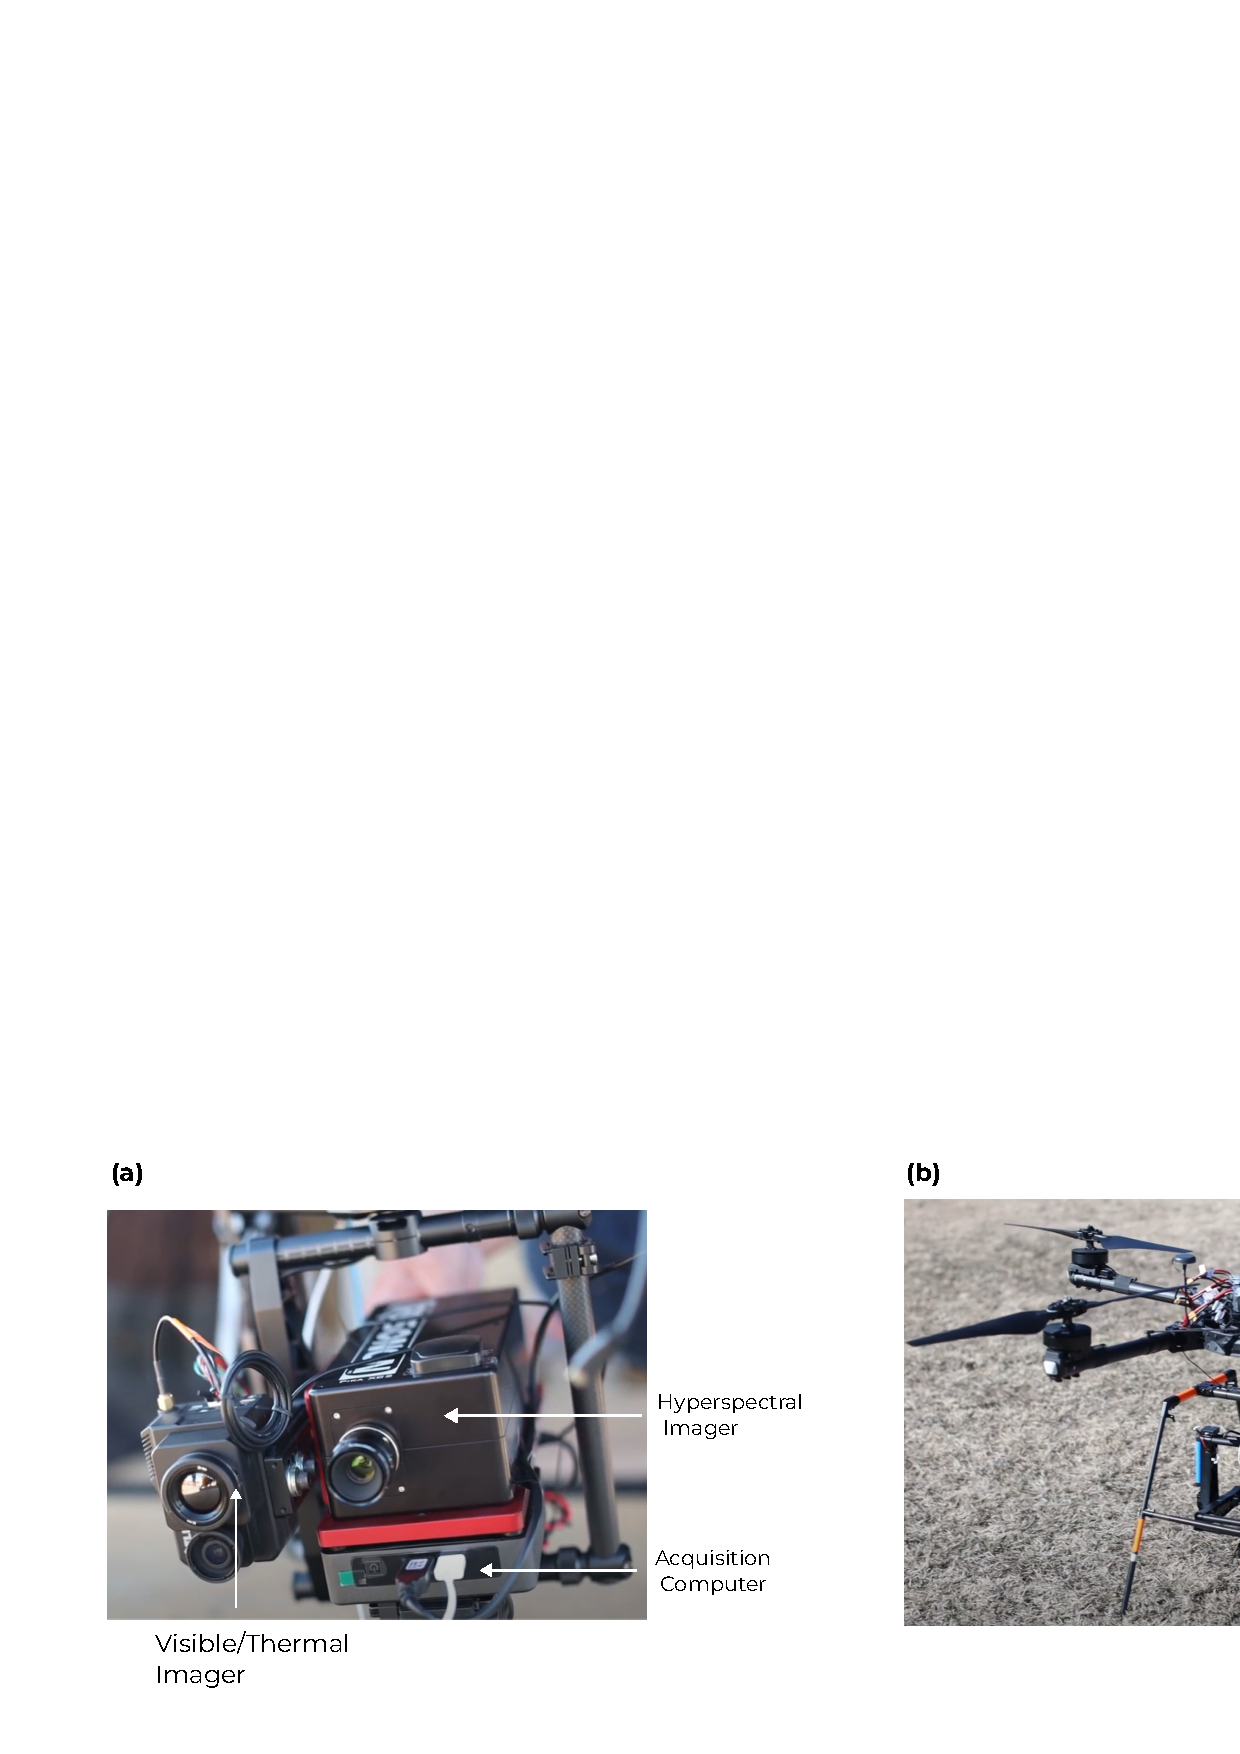
\includegraphics[width=0.85\columnwidth]{robot-team/assets/annotated-drone.pdf}
    \caption{Components of the Autonomous Drone HSI platform.}
    \label{fig:drone-components}
\end{figure}


\subsection{Real time processing of HSI imagery}

- overview of processing pipeline

\begin{figure}[h]
    \centering
    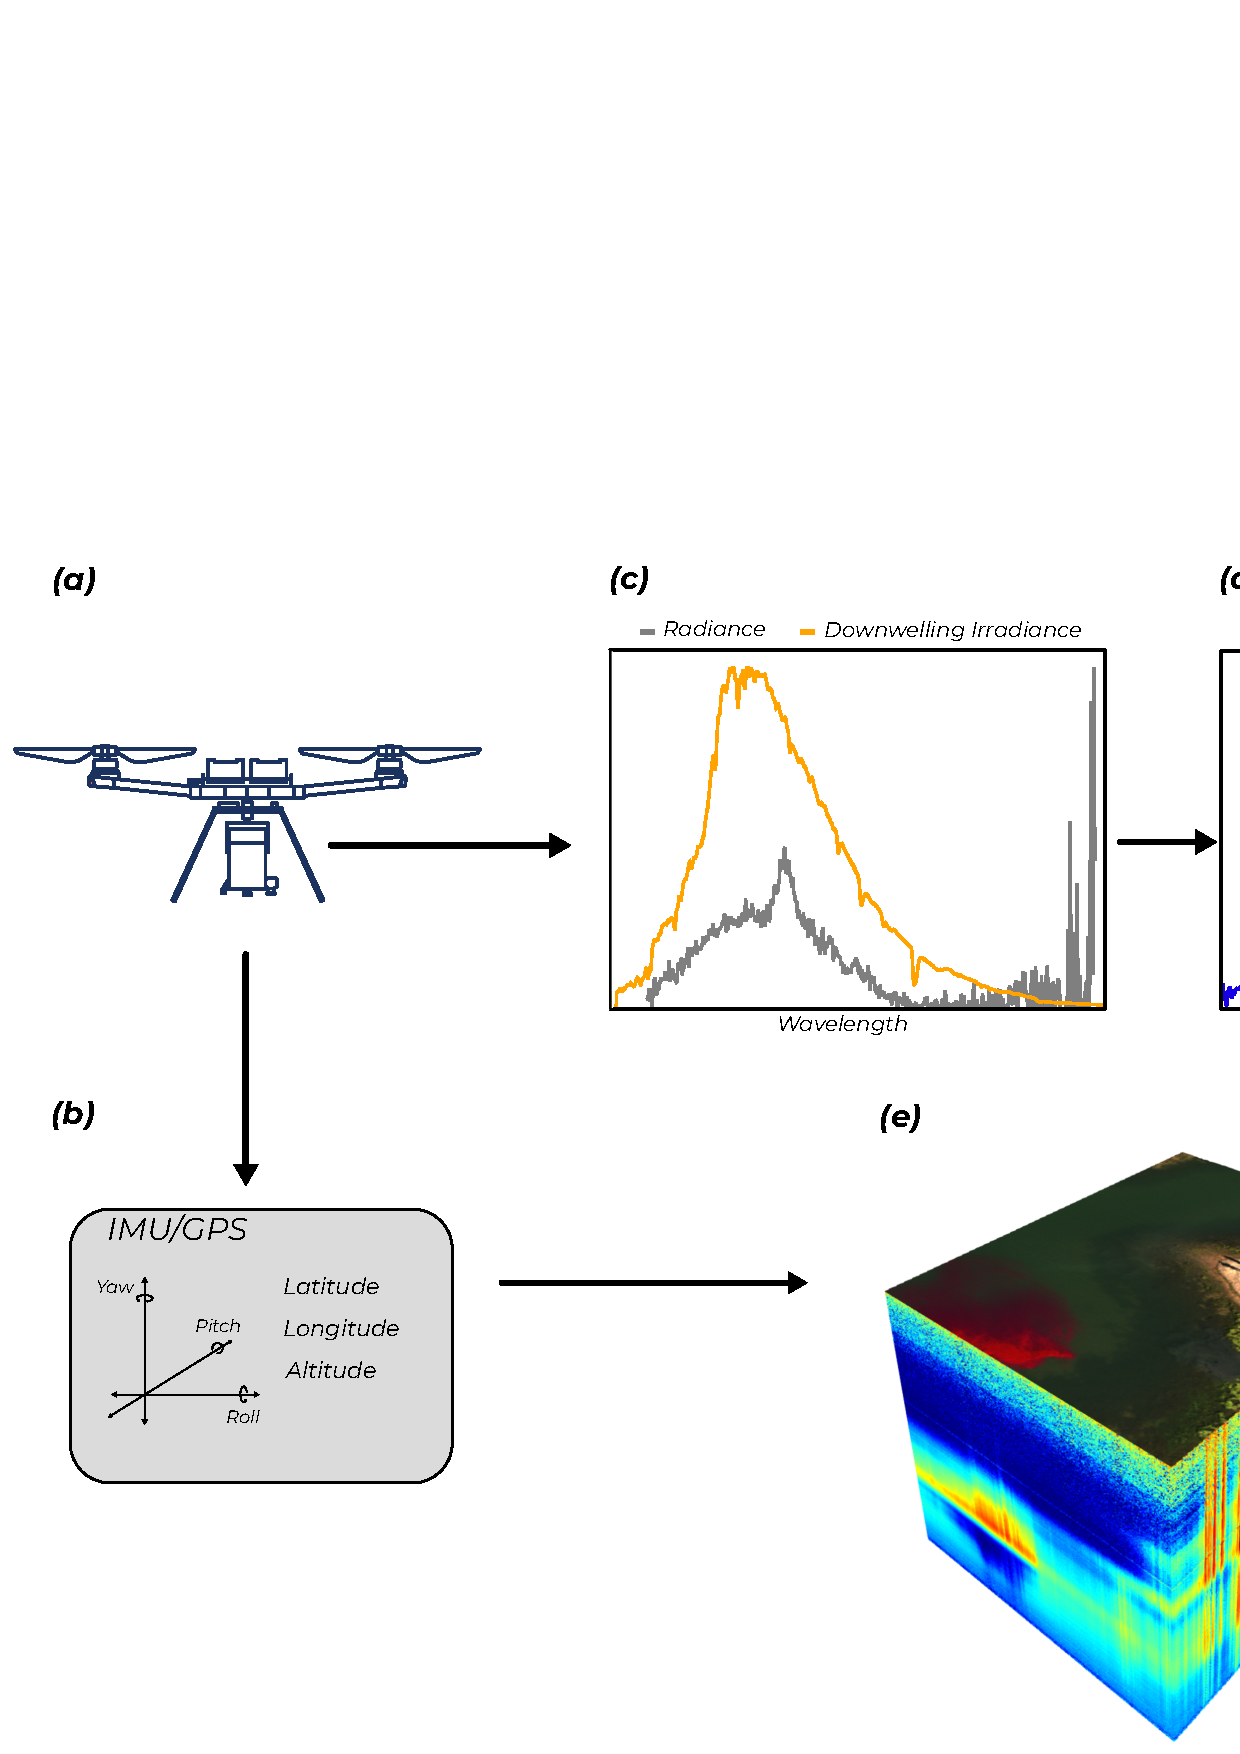
\includegraphics[width=0.85\columnwidth]{robot-team/georectification/pipeline-figure.pdf}
    \caption{Solar Irradiance spectrum captured by downwelling spectrometer.}
    \label{fig:annotated-hsi}
\end{figure}

- Collection of raw HSI by imager
- Reading stored binary (ENVI) radiance data into tensor
- Reading Flight Data 
- Interpolate flight data from IMU to match HSI times
- Reading stored downwelling irradiance spectrum 
- Interpolate irradiance spectrum to match HSI $\lambda$s 
- Conversion to Reflectance under the assumption of a Lambertian surface (perfectly diffuse)
- Georectify to obtain new coordinates
- resample to regular grid
- compute derived $\lambda$-metrics (NDVI, etc...) 
- serve result (save to HDF5 or serve via web map service over wifi) 


Georectification Procedure.
\begin{itemize}
    \item collect datacube 
    \item read HSI in ENVI format
    \item read Flight Data 
    \item interpolate flight data to HSI times 
    \item read Downwelling irradiance spectrum
    \item convert radiance to reflectance 
    \item georectify to obtain new coordinates 
    \item resample to regular grid
    \item save results to HDF5
\end{itemize}

Code and data availability via OSN and Github


\subsection{Georectification Procedure}


\begin{figure}[h]
    \centering
    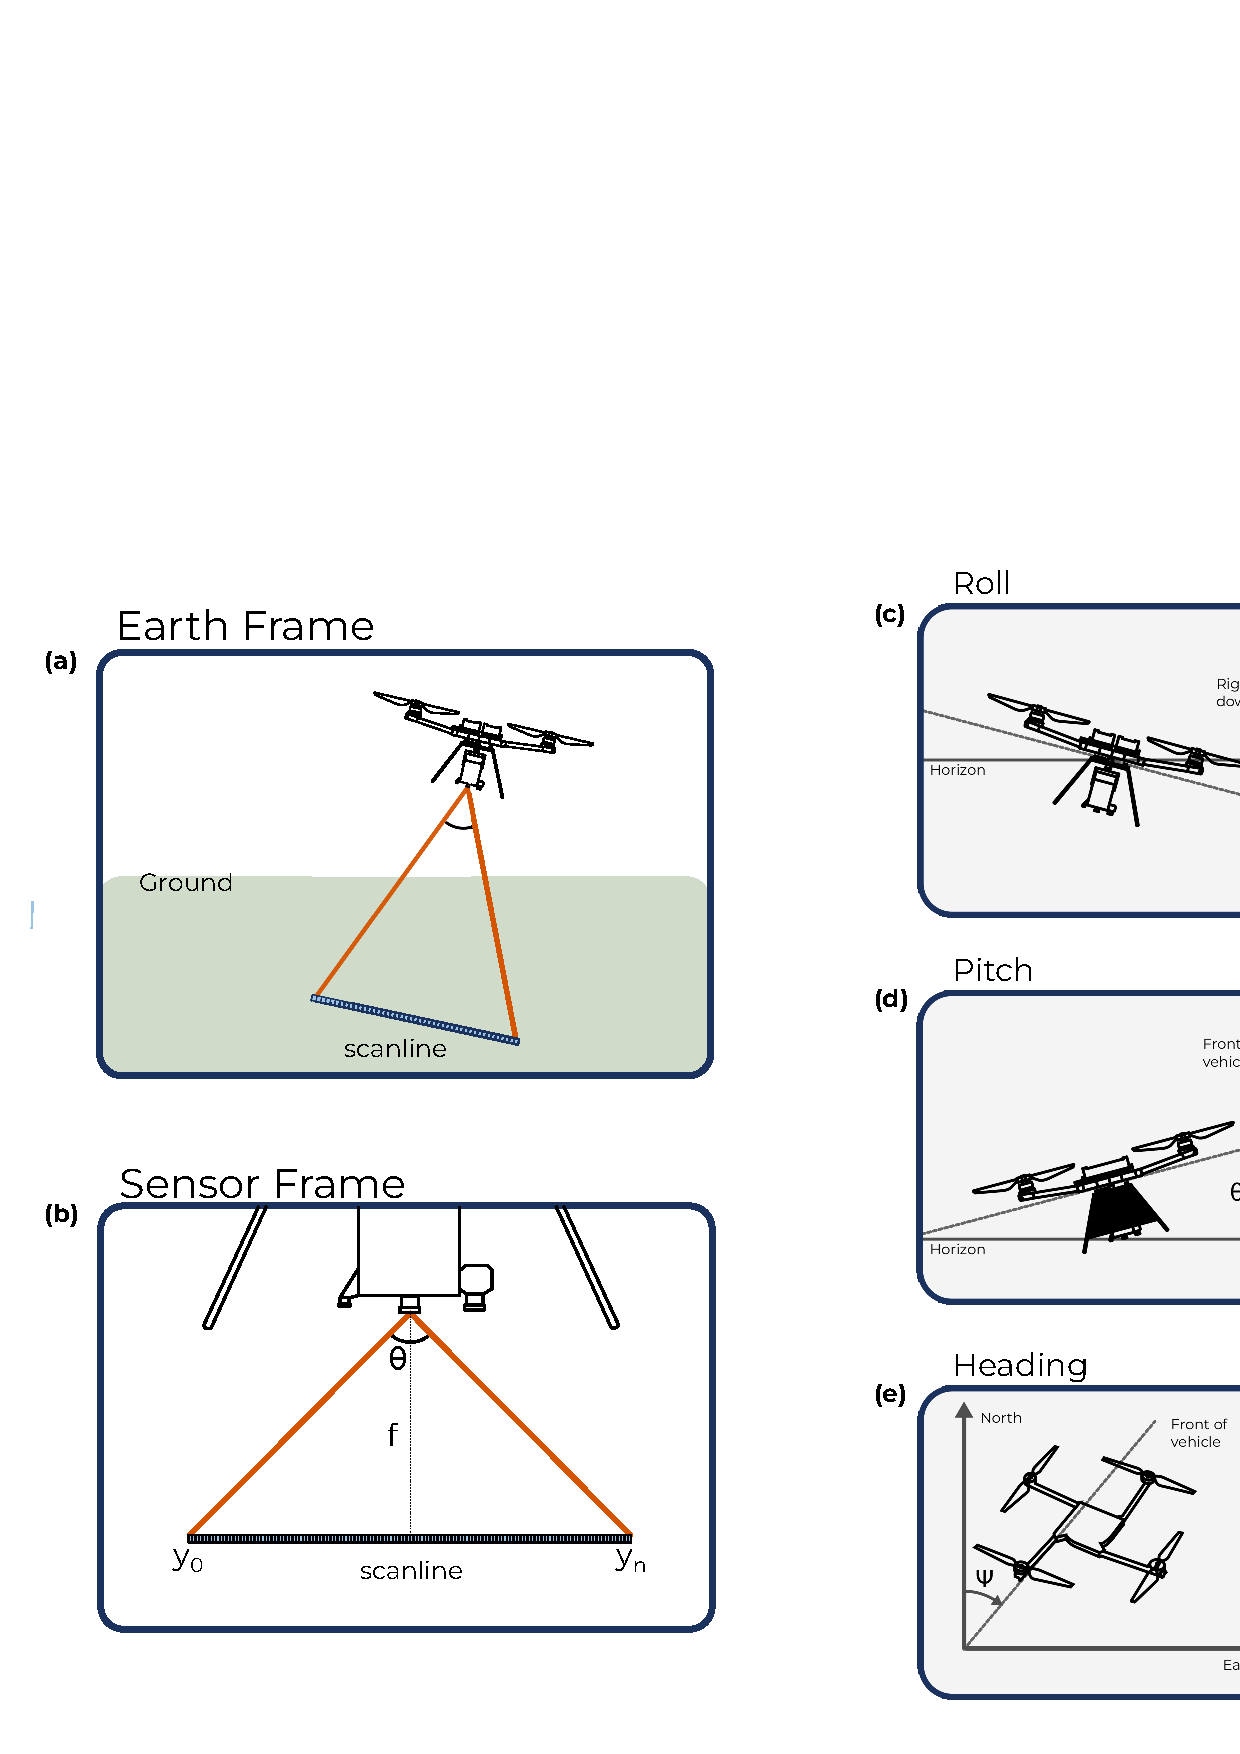
\includegraphics[width=0.85\columnwidth]{robot-team/assets/georectification.pdf}
    \caption{Visual representation of scan-line geometry for the drone based hyperspectral imaging platform.}
    \label{fig:georectification}
\end{figure}


%%%%%%%%%%%%%%%%%%%%%%%%%%%%%%%%%%%%%%%%%%
\section{Results}

\begin{figure}[h]
    \centering
    \includegraphics[width=0.85\columnwidth]{robot-team/georectification/hsi-infographic.pdf}
    \caption{Annotated view of a hyperspectral data cube showcasing sampled spectra for a variety of constituents.\label{fig:hsi-infographic}}
\end{figure}  


\begin{figure}[h]
    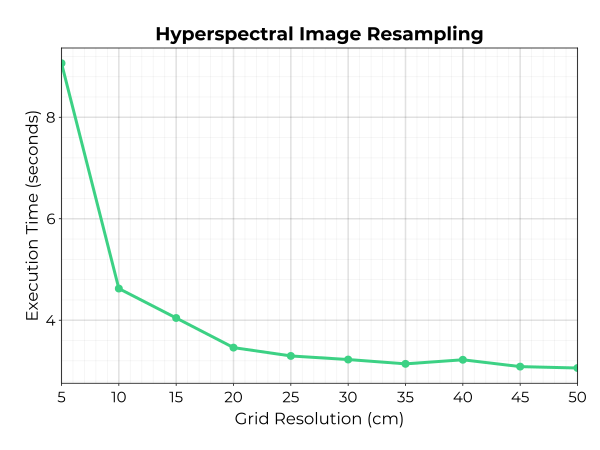
\includegraphics[width=0.85\columnwidth]{robot-team/georectification/regrid-timing.pdf}
    \caption{This is a figure. Schemes follow the same formatting. If there are multiple panels, they should be listed as: (\textbf{a}) Description of what is contained in the first panel. (\textbf{b}) Description of what is contained in the second panel. Figures should be placed in the main text near to the first time they are cited. A caption on a single line should be centered.}
    \label{fig-regridding-timing}
\end{figure}

\begin{figure}[h]
  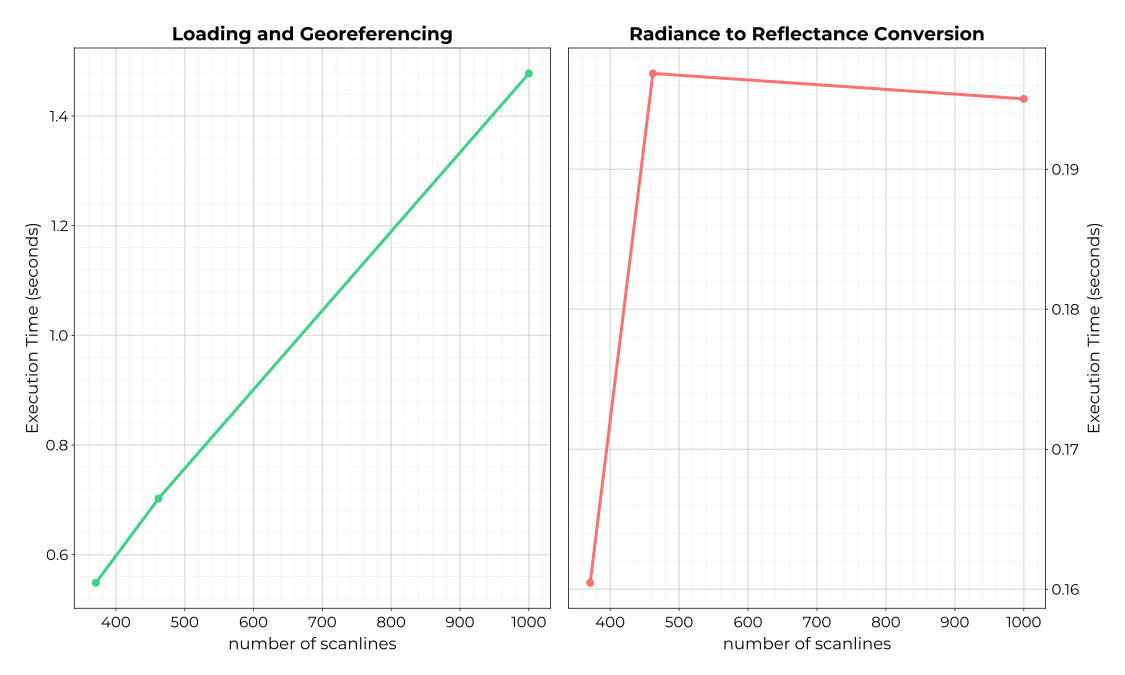
\includegraphics[width=0.95\columnwidth]{robot-team/georectification/reflectance-timing.pdf}
  \caption{Description}
  \label{fig-reflectance-timing}
\end{figure}

NOTE: we need to update these timings by first copying the HSI to the local drive (off of the external hard drive). This will probably have some effect on the read/write speeds for the test.

%% \begin{table}[h]
%% \caption{Resampling times as a function of pixel resolution.\label{tab1}}
%% \newcolumntype{C}{>{\centering\arraybackslash}X}
%% \begin{tabularx}{\textwidth}{CC}
%% \toprule
%% \textbf{Resolution (m)}	& \textbf{Execution time (s)}\\
%% \midrule
%% 0.5		&   1.434	\\
%% 0.4     &   1.545	\\
%% 0.3     &   1.673   \\
%% 0.2     &   1.802   \\
%% 0.1     &   4.026   \\
%% 0.05    &   10.537  \\
%% \bottomrule
%% \end{tabularx}
%% \end{table}


%% \begin{table}[h]
%%   \caption{Loading and Reflectance Conversion Times.\label{tab1}}
%%   \newcolumntype{C}{>{\centering\arraybackslash}X}
%%   \begin{tabularx}{\textwidth}{CC}
%%     \toprule
%%     \textbf{Number of scan lines}	& \textbf{Execution time (s)}\\
%%     \midrule
%%     371		&   2.060	\\
%%     725     &   4.227	\\
%%     1000    &   5.901   \\
%%     \bottomrule
%%   \end{tabularx}
%% \end{table}




\textbf{NOTE} Stuff to do in this section:
\begin{itemize}
    \item  Create table with processing timings for each step on a typical HSI
    \item Create second table comparing time for full processing including resampling to a variety of scales (e.g. 5 cm, 10 cm, 25 cm) We will want a version of the processing function that does not include the uncertainties and the spectral indices
    \item create pipeline visualization showing size of each of the data products and their step in the pipeline (ending with a dataproduct like the NDVI)
    \item Create a figure showing the georeferenced image on top of the satellite background 
    \item Create another figure of the entire map with a spectral index applied to one of the dye-release datasets (to demonstrate use for real-time application like oil-spill)
    \item create a figure of a sample HSI datacube in 3-d like from the previous paper with the rgb image on the top. 
\end{itemize}



%%%%%%%%%%%%%%%%%%%%%%%%%%%%%%%%%%%%%%%%%%
\section{Discussion}

- Incorporation of drone into autonomous robotic team
- Long range wireless network (ubiquiti) for data downlink
- Incorporation of edge-ML for direct determination of chemical concentration
- Utility for navigation, waste removal, etc...

Discuss drawbacks (striping in images) 

Authors should discuss the results and how they can be interpreted from the perspective of previous studies and of the working hypotheses. The findings and their implications should be discussed in the broadest context possible. Future research directions may also be highlighted.




\section{Supervised Regression with Uncertainty Quantification}

\subsection{Hyperspectral Imaging and Remote Sensing}
paper creating new spectral index for wheat rust \cite{SpectralIndexWheat} \\ 
overview of NDVI \cite{SpectralIndexNDVI} \\ 
paper using spectral indices for desertification \cite{SpectralIndexDesertification}


\subsubsection{HSI sattelite systems}
\subsubsection{HSI drone systems}
\subsubsection{Machine Learning using HSI}
add Xiao He reference here \cite{yu2021pm2}

\subsection{In-situ Measurements / Robot Teams}
\subsubsection{Meteorology}
\subsubsection{Atmospheric Sensing}
add in reference to our AQ sensor network

\subsection{Julia Programming Language}
\subsubsection{scientific computing}
\subsubsection{differentiable programming ($\partial P$)}
\subsubsection{MLJ}
discuss general \textit{learning network} framework and utilization of
Directed Acyclic Graphs for pipeline construction

basic overview of MLJ as a Julia package \cite{MLJ1}\\ 

detailed description of \textit{learning networks} \cite{MLJ2}



\section{Materials and Methods}
\subsection{Autonomous Collection and Processing of Hyperspectral Images}

website for alta x \cite{freeflyAltaX}

\begin{equation}
  R = \pi \frac{L}{E}
\end{equation}



\subsection{Georectification}
paper by Muller \cite{muller-georeferencing} \\
paper by Baumker \cite{GeorectificationBaumker} \\
paper by Mostafa \cite{GeorectificationMostafa} \\



NOTE: need to double check \cite{muller-georeferencing} for convention used ($\Phi$ vs $\phi$)

Heading correction due to longitude deviation in UTM system:
\begin{equation}
  \kappa_{\text{geodetic}} = \kappa_{\text{geographic}}-\tan^{-1}\left( \sin\Phi \tan(\lambda-\lambda_{cm}) \right)
\end{equation}

scale factor:
\begin{equation}
  s = \frac{z_{\text{sensor}}-z_{\text{ground}}}{f}
\end{equation}

\begin{equation}
  \begin{pmatrix}
    x \\ y \\ z
  \end{pmatrix}_{\text{Object}}^{\text{UTM}} =
  f_{\text{geo}}^{\text{UTM}}\begin{pmatrix}
    \lambda \\
    \Phi \\
    z
  \end{pmatrix}_{\text{GPS}}^{\text{geo}} + sT_{\text{IMU}}^{\text{UTM}}R_{\text{sensor}}^{\text{IMU}}(\kappa, \phi, \omega)\begin{pmatrix}
    0 \\
    y_i \\
    f
  \end{pmatrix}_{\text{object}}^{\text{sensor}}
\end{equation}




\subsection{In-situ Data Collection via Robotic Sentinels}

autonomous boat website \cite{Otter}


\subsubsection{data collection process}
\subsubsection{Data Collocation}

\subsubsection{CO}
\subsubsection{CDOM}
\subsubsection{HDO}
\subsubsection{$Na^{+}$}
\subsubsection{$Ca^{2+}$}
\subsubsection{Other Targets}

\subsubsection{Feature Engineering with Remote Sensing Indices}
include discussion of PCA as well as Standardization


\subsection{Exploratory Data Analysis}
\subsubsection{Variable Correlations}

\begin{figure}[h]
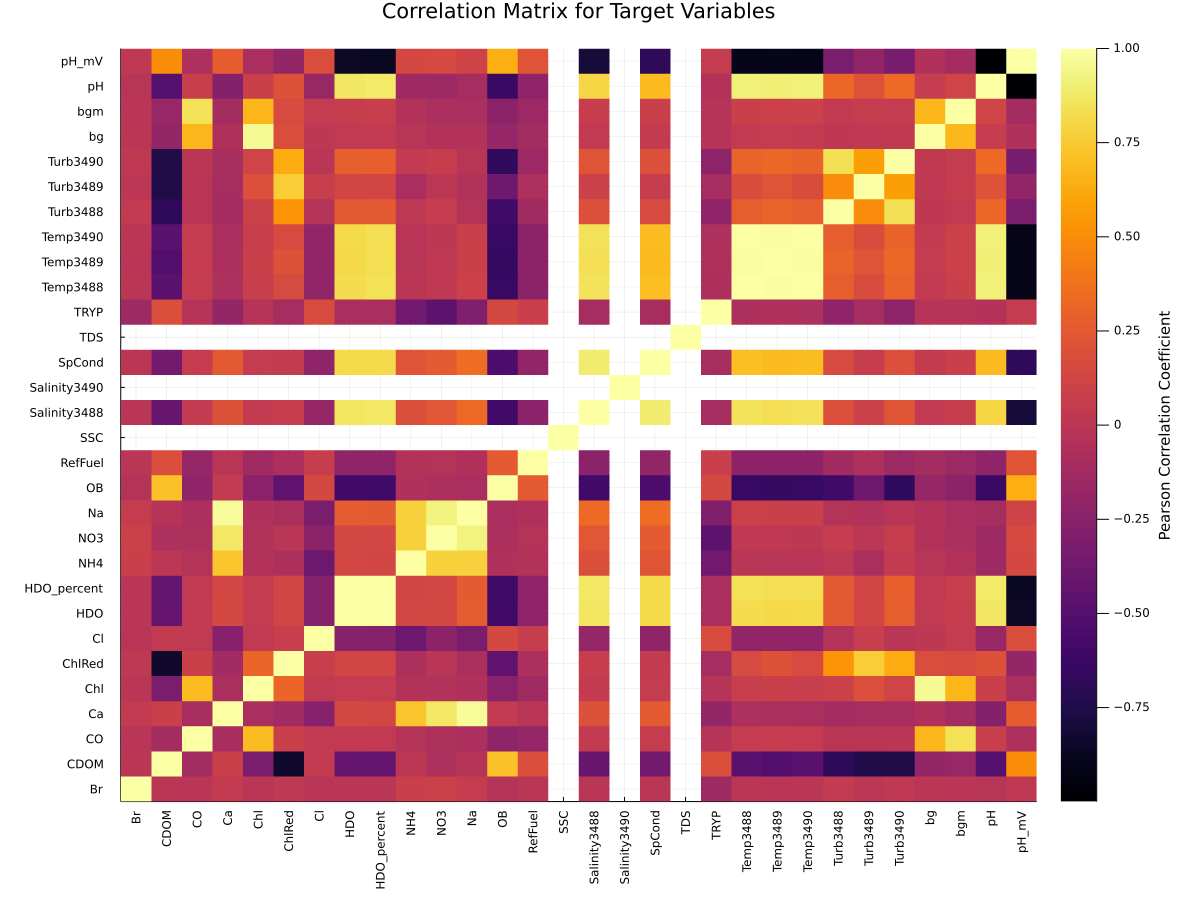
\includegraphics[width=0.85\columnwidth]{robot-team/supervised-2/correlation/target_cor.png}
\caption{Correlation Matrix for Target variables measured by the boat.\label{target_cor}}
\end{figure}

\begin{figure}[h]
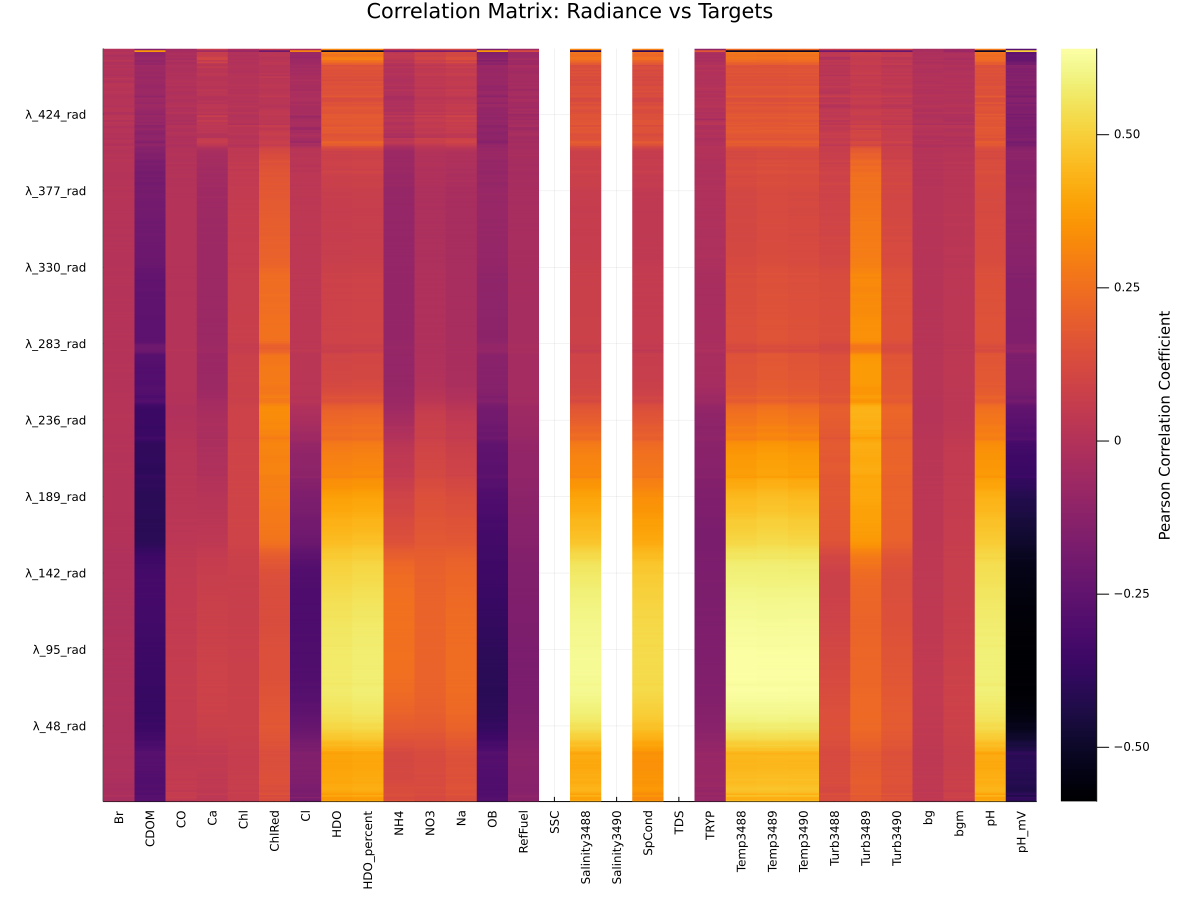
\includegraphics[width=0.85\columnwidth]{robot-team/supervised-2/correlation/radiance_cor.png}
\caption{Correlation Matrix for Radiance measurements versus Target Variables.\label{rad_cor}}
\end{figure}

\begin{figure}[h]
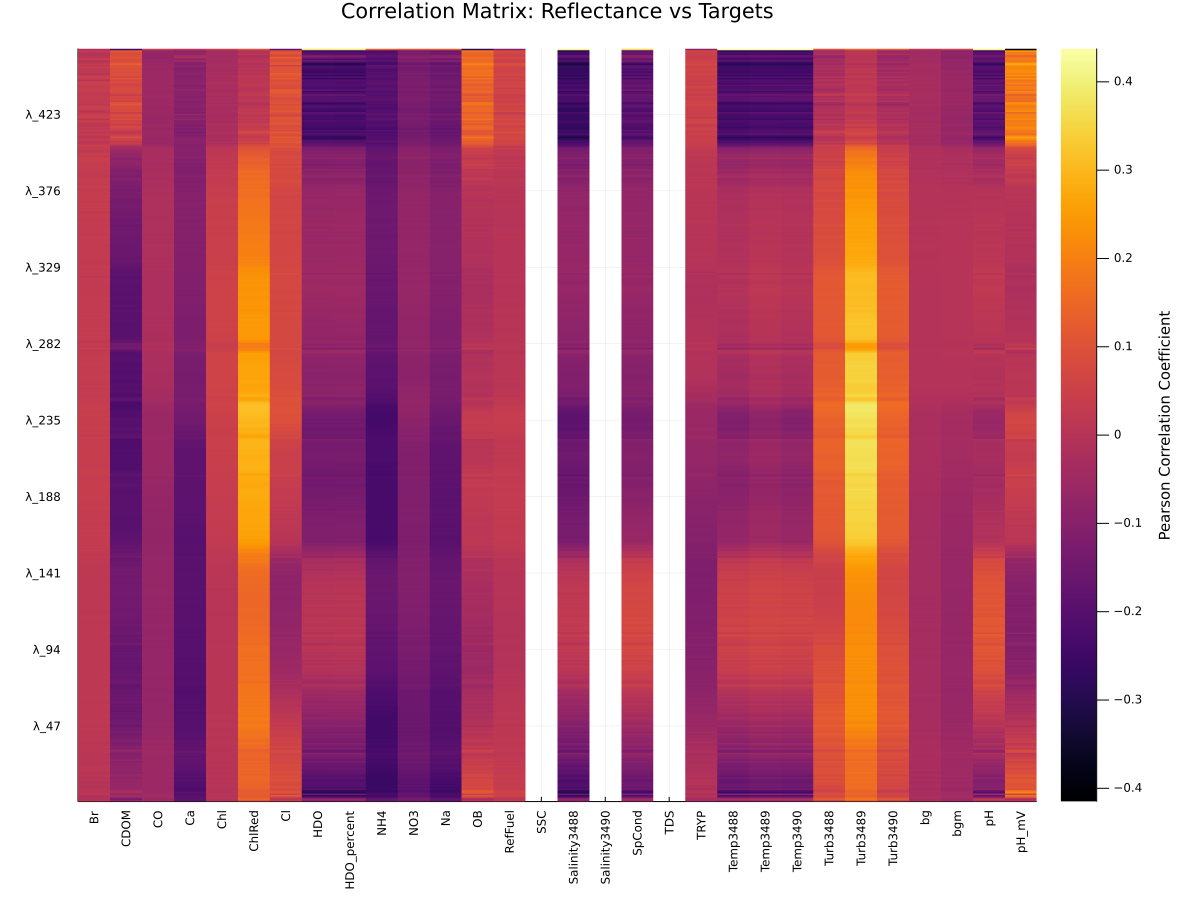
\includegraphics[width=0.85\columnwidth]{robot-team/supervised-2/correlation/reflectance_cor.png}
\caption{Correlation Matrix for Reflectance measurements versus Target Variables.\label{ref_cor}}
\end{figure}

\begin{figure}[h]
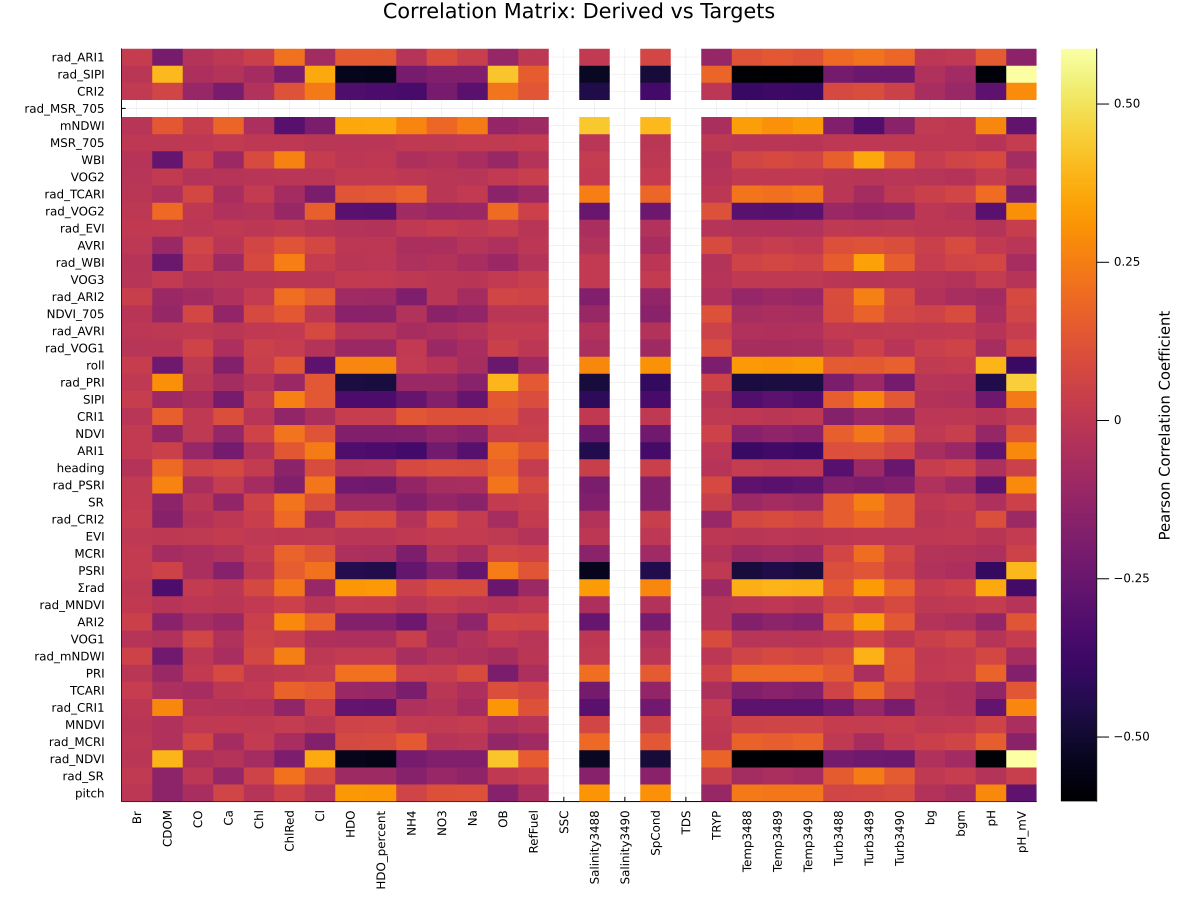
\includegraphics[width=0.85\columnwidth]{robot-team/supervised-2/correlation/derived_cor.png}
\caption{Correlation Matrix for derived measurements versus Target Variables.\label{derived_cor}}
\end{figure}



\subsubsection{Machine Learning Models}
include Linear Models, Neural Networks, Decision Trees, Bagging, Boosting, and Stacking\\

The field of Machine Learning has seen the invention of a plethora of models able to perform inference for regression tasks. Naturally, this leads to the challenge of evaluating which model is best for a given problem. In 1992 David Wolpert developed the notion of Stacked Generalization to divorce arbitrary human choice from the model selection process. [1] The key idea is as follows: fit an instance of each model compatible with your dataset. Each model learns different features of the data so that an adjudicating model (called the super-learner) can then be trained to map the predictions from each individual learner to a final output prediction. This is incredibly easy to accomplish in the Julia programming language via the MLJ machine learning framework [2]. We train a variety of learners including artificial neural networks, bagged decision trees, boosted decision trees, polynomial regressors, quantile regressors, LASSO regressors, and K-nearest-neighbors regressors. To ensure proper data hygiene, individual learners are first trained on separate cross validation folds so as not to bias the super-learner. After training the super-learner, each individual model is then trained on the full dataset to produce the best possible model.


paper on stacking \cite{ModelStacking}

\subsection{Model Analysis}
aleatoric and epistemic uncertainty

The black-box nature most machine learning methods makes it difficult to consider how errors propagate through a trained model during the inference process. For many problems such as image classification this is not an issue, however, in physical sensing error considerations are vital to establish detection limits and prediction confidence. Typically, there are three considerations we must make: measurement uncertainty– how much we can trust our model’s inputs, measurement representativeness– how well each data point represents data within a local neighborhood, and model error– how far the prediction is from the true value. Machine learning models are typically trained to minimize the model error. The Julia programming language makes it possible to handle all three. 


To address measurement uncertainty, we take advantage of Julia’s advanced automatic differentiation capabilities to enable differentiable programming (∂P). This means that we can take derivatives of our trained ML model with respect to each input feature to perform a sensitivity analysis. The final output uncertainty is then given via linear error propagation theory. [5]

Measurement representativeness can be trickier to handle. For example, in fluids it is common for two species to form a mixing layer that presents as a sharp discontinuity in measurement values. To quantify the degree to which neighboring points diverge we compute the average deviation across input measurements in a neighborhood around each data sample. This information can then be presented with model outputs to identify the regions where our model is valid. Similarly for ensemble ML models we compute the prediction deviation across all base learners to identify the representativeness of a data sample. Inputs that cause a large spread in base learner predictions indicate low representativeness in the training set. This analysis can then be used to plan further data collection missions that minimize time spent collecting data we have already present in our models. 

\subsubsection{Uncertainty Propagation via ($\partial P$)}

\subsubsection{Feature Ranking via SHAP values}

shape value paper used in ShapML.jl \cite{SHAPvalues1}

\subsubsection{Data Representativeness}
i.e. the average deviation across pixels used average during collocation process.
Also, we can look at relative disagreement between model predictions in bagged ensemble. 

\section{Results}
\subsection{CO}

\begin{figure}[h]
\includegraphics[width=0.85\columnwidth]{robot-team/supervised-2/CO/CO_dataMap.png}
\caption{Target distribution of CO at Scotty's Ranch.\label{CO_targetMap}}
\end{figure}

\begin{figure}[h]
\includegraphics[width=0.85\columnwidth]{robot-team/supervised-2/CO/CO_train-test_hist.png}
\caption{Stratified train-test split for CO.\label{CO_trainTestHist}}
\end{figure}

\begin{figure}[h]
  \begin{subfigure}{0.5\textwidth}
    \centering
    \includegraphics[width=0.95\linewidth]{robot-team/supervised-2/CO/rfr_CO_scatter.png}
  \end{subfigure}
  \begin{subfigure}{0.5\textwidth}
    \centering
    \includegraphics[width=0.95\linewidth]{robot-team/supervised-2/CO/rfr_CO_qq.png}
  \end{subfigure}
  \caption{(\textbf{a}) Scatterplot for the trained random forest Crudo Oil model. (\textbf{b}) Quantile-Quantile plot for the same fit.}
  \label{CO_fitresult}
\end{figure}



\begin{figure}[h]
    \includegraphics[width=0.85\columnwidth]{robot-team/supervised-2/CO/rfr_CO_featureImportance.png}
    \caption{Ranked feature importance for Crude Oil. Importance is determined via mean absolute SHAP value. \label{CO_shapely}}
\end{figure}






\section{Methods for Unsupervised Classification of Hyperspectral Scenes in Novel Environments}

\subsubsection{Unsupervised Classification}
\begin{figure}[h]
  \includegraphics[width=0.85\columnwidth]{robot-team/unsupervised/clustering.png}
  \caption{Unsupervised clustering of hyper-spectral image data using the K-means algorithm.\label{clustering}}
\end{figure}




%% \chapter{A Distributed Network of Low Cost Air Quality Sensors}

\section{MINTS Air Quality Network}
\subsection{Central Nodes}
\subsection{LoRa Nodes}
\subsection{MQTT}

\section{Real Time Dashboards via Containerization}

\section{Making Data Publicly Accessible via S3 and the Open Storage Network}
discuss Rclone and using OSN to make data highly available


\begin{itemize}
\item LoRa wan devices
\item Docker, NodeRed, InfluxDB, Grafana
\item Hamiltonian NN stuff
\item neural ode
\item TDA
\end{itemize}

Sensor Network + SciML
Evaluation of local chaos in SharedAirDFWNetwork

\begin{itemize}
\item This gives me an excuse to work with the sensor data
\item Train GTM, SOM, and Variational Autoencoder to produce lower dimensional representation of all data from a central node, e.g. in $\mathbb{R}^2$.
\item For VAE, test a range of dimensions from the number of sensors down to 2 (better for visualization)
\item Analyze the variety of methods from [DataDrivenDiffEq.jl](https://docs.sciml.ai/DataDrivenDiffEq/stable/) to infer dynamics in the low dimensional space
\item Can we infer some kind of Hamiltonian from the data and do a HamiltonianNN approach?
\item Start of with a standard kinetic-energy style Hamiltonian e.g. $\sum_i \frac{1}{2} \dot{x}_i^2$ where $x_i$ is the
\item use DataDrivenDiffEq approach to learn the associated potential energy term
\item alternatively, attempt to capture diurnal cycle (or other relevant time scales) by *learning* coordinate representation that forces dynamics to be uncoupled harmonic oscillators a la Hamilton-Jacobi theory.
\item Test if this hamiltonian NN model can then be transfered to another central node with an appropriate shift in the "total energy"
\item Attempt to analyze the 2d data to infer Koopman operator. We should treat the original sensor values as observables on which the learned koopman operator acts. This should be doable if the NN is just a function.
\item use DMD appraoch to identify a "forcing" coordinate that can identify when we switch nodes as in \cite{brunton-havok}
\item \href{https://www.youtube.com/watch?v=lx-msllg1kU&ab_channel=SteveBrunton}{video on Physics Informed DMD}
\item \href{https://www.youtube.com/watch?v=KmQkDgu-Qp0&list=PLMrJAkhIeNNQ0BaKuBKY43k4xMo6NSbBa&ab_channel=SteveBrunton}{Deep Learning to Discover Coordinates for Dynamics: Autoencoders and Physics Informed Machine Learning}
\item \textbf{NOTE:} we may need to impute missing values. We shoud do so with either my GPR code or with other ML methods + ConformalPrediction. Provided uncertainty estimates, we should then think about how to propagate errors through our analysis via \href{https://github.com/JuliaPhysics/Measurements.jl}{Measurements.jl}, \href{https://juliaintervals.github.io/pages/packages/intervalarithmetic/}{IntervalArithmetic.jl}.
\end{itemize}

\chapter{Time Series Methods for Air Quality}

With the proliferation of low-cost sensors for a wide range of IoT and wearable biometric applications, a systematic approach to both quality control and performing comprehensive time series analysis has significant value. It is highly desirable to be able to answer some basic questions using \textit{just} the time series alone. For example: What is the likely sensor uncertainty given a time series of observations? How frequently should observations be made to adequately resolve typical temporal variability? How representative is a single observation of what one expects to see over a temporal (and spatial) window? Can we construct predictive models for the time series of a single sensor given a sufficient volume of sample data? In this chapter we seek to address these questions with direct application to the data collected by our low cost air quality sensor network. First, we will demonstrate how the \textit{temporal variogram} provides a way to assess the intrinsic sensor uncertainty from a time series, and in the process, develop an open-source Julia implementation of a variety of variogram methods that can be used for any generic time series. Next, we present two techniques for physics-based time series modeling: the Hankel Alternative View Of Koopman (HAVOK) method, and the Hamiltonian Neural Network. It should be noted that despite the rapid pace of development in the fields of data-driven and scientific machine learning, many recently developed techniques like the Universal Differential Equations (UDEs), Hamiltonian Neural Networks, and others have yet to see application on noisy real-world datasets. Our secondary goal for this chapter is therefore to demonstrate how with some slight modifications, these techniques can find to real scientific problems.



\section{Time-Series Methods for Uncertainty Quantification}

As we've already demonstrated, the shrinking cost of sensing technologies has improved our ability to create dense sensing networks. In order to make effective use of these sensors, and to provide high quality data that can be used for critical decision making, it is vital we establish both the relevant sampling time scale and reasonable uncertainty estimates for measurements obtained by these sensors. For low cost sensors in particular, the manufacture supplied uncertainty estimates tend to be highly conservative so as to minimize their responsibility for variation in device performance, and in general, to prevent unnecessary returns. Consider for example, the sample time series for particulate matter concentrations at a variety of size fractions collected by one of our low-cost sensing nodes for a single 24-hour period (figure \ref{fig:pm-single-day}:
\begin{figure}[h]
  \centering
  \includegraphics[width=0.85\columnwidth]{time-series/variogram/single-day/IPS_single-day.pdf}
  \caption{Time series of particulate matter at size fractions $1.0$, $2.5$, and $10.0$ $\mu m$ captured at a single location over one 24-hour day.}
  \label{fig:pm-single-day}
\end{figure}
These sample data illustrate many typical features of air quality time series: there is a baseline level of noise, there are general periodic trends (an increase in concentration at all size fractions near morning traffic around hour 10), and there are intermittent transient events. If we suppose that we \textit{already} know what the shortest time resolution needed to resolve the important transients is, say $\Delta t$, then a straight forward approach to develop a baseline notion of uncertainty for a time series, $z(t)$, is to convolve a rolling window of width $\Delta t$ across the signal so that at any time $t$ we may define the associated \textit{pseudo-observation} to be
\begin{equation}
  \bar{z}(t) = \text{mean}\left(\left\{z_j \right\}\right) \pm \text{std}\left(\left\{z_j \right\}\right); \quad \text{where } j \in \left\{ \left. j \right\vert t - \frac{\Delta t}{2} \leq t_j  \leq t + \frac{\Delta t}{2}\right\}
\end{equation}
where $\text{std}\left(\left\{z_j\right\}\right)$ is called the \textit{representativeness uncertainty} as it measures how representative a single measurement is for the entire sampling window.

Unfortunately it may be difficult to know the relevant times scales of key transient events in advance. Given the fact that it is increasingly common for modern sensing systems (like our low-cost PM monitors) to provide sampling rates north of 1 Hz, we do not want to \textit{shoot ourselves in the foot} by arbitrarily choosing an averaging window that will smooth away all the relevant features. Therefore, we seek to develop an alternative technique that can simultaneously establish the relevant temporal resolution for sampling whilst also enabling us to estimate the aleatoric, that is, intrinsic uncertainty of the sensing system.

\subsection{Uncertainty Quantification with Temporal Variograms}

The key feature that differentiates time series from other data sources is that at short time scales, neighboring samples are not independent; measurements taken close in time tend to be more correlated than measurements taken far apart. One way to measure this idea of self-similarity is by the auto-correlation function, which for a continuous signal $z(t)$ is
\begin{equation}
  R_{zz}(\Delta t) = \int_\infty^\infty z(t +\Delta t)z^*(\Delta t)dt.
\end{equation}
This can be efficiently computed for real-valued time series in $\mathcal{O}(n\log n)$ using the \textit{Fast Fourier Transform} via
\begin{equation}
  R_{zz}(\Delta t) = \mathcal{F}^{-1}\left[\mathcal{F}(z)\cdot (\mathcal{F}(z))^*\right]
\end{equation}
The first peak of this autocorrelation function is an excellent method to identify the relevant time-scale: high autocorrelation means we gain little extra information between points offset by a time lag of $\Delta t$. This puts us on the right track but does not provide a straight forward interpretation for an intrinsic uncertainty. Taking motivation from the representativeness uncertainty, let us instead consider the expected variance between neighboring samples as a function of the time lag $\Delta t$. That is,
\begin{equation}
  2\gamma(\Delta t) =  \text{Var}\left(z(t+\Delta t) - z(t)\right)
\end{equation}
where $\gamma$ is called the \textit{semi-variogram} for $z(t)$. Expanding this definition yields
\begin{equation}
  2\gamma(\Delta t) = \E\left[\left(z(t+\delta t) - z(t) - \E\left(z(t+\Delta t) - z(t) \right) \right)^2 \right]
\end{equation}
which for timescales where $z(t)$ is sufficiently stationary simplifies to yield
\begin{equation}
  \gamma(\Delta t) = \frac{1}{2}\E\left[ \left(z(t+\Delta t) - z(t) \right)^2\right].
\end{equation}

For a perfect measurement system we would expect that taking $\lim_{\Delta t \to 0}\gamma(\Delta t) = 0$, since measurements taken at the same time by the same instrument \textit{should} be identical. Intrinsic uncertainty will therefore manifest as a non-zero limit and taking the square-root of the variogram will yield units that match our original time series and provide a reasonable uncertainty estimate. For a given set of samples, we construct the \textit{empircal variogram} as
\begin{equation}
  \hat{\gamma}(\Delta t) = \frac{1}{2N(\Delta t)}\sum_i^{N(\Delta t)}\left(z(t_i + \Delta t) - z(t_i) \right)^2
\end{equation}
where $N(\Delta t)$ are the number of available observation pairs $(z_i, z(t_i+\Delta t))$ for a lag of $\Delta t$.

There are three key parameters of the variogram $\gamma(\Delta t)$ which we want to estimate from $\hat{\gamma}(\Delta t)$:
\begin{itemize}
\item \textbf{Nugget}: The $y$-intercept of $\gamma(\Delta t)$ representing the limit as $\Delta t \to 0$.
\item \textbf{Sill}: The value of $\gamma(\Delta t)$ as $\Delta t \to \infty$. In other words, the expected variance for uncorrelated samples of our time series. \textit{Note} the \textbf{partial sill} is defined to be the sill minus the nugget.
\item \textbf{Range}: The $\Delta t$ at which $\gamma$ realizes it asymptote. Effectively this is the time lag beyond which samples are uncorrelated and can be used as a proxy for the relevant sampling time scale.
\end{itemize}

To do this, we first compute $\hat{\gamma}(\Delta t)$ as above and then fit a model to $\gamma(\Delta t)$. There are a number of popular choices depending on the structure of a particular time series. In my open source Julia implementation, \texttt{TimeSeriesTools.jl}, the following models are made available:
\begin{itemize}
\item \textbf{Spherical}:
  \begin{equation}
    \gamma(\Delta t) = b + C_0\left(1.5\frac{\Delta t}{r} - 0.5 \frac{(\Delta t)^2}{r^2} \right)
  \end{equation}
\item \textbf{Exponential}:
  \begin{equation}
    \gamma(\Delta t) = b + C_0\left( 1 - \exp\left(-\frac{\Delta t}{r}\right)\right)
  \end{equation}
\item \textbf{Gaussian}:
  \begin{equation}
    \gamma(\Delta t) = b + C_0\left( 1 - \exp\left(-\frac{(\Delta t)^2}{r^2}\right)\right)
  \end{equation}
\item \textbf{Circular}:
  \begin{equation}
    \gamma(\Delta t) = b + C_0\left(1 - (2\pi)\cos^{-1}\left(\frac{\Delta t}{r}\right) + \frac{2\Delta t}{\pi r}\sqrt{1-\frac{(\Delta t)^2}{r^2}} \right)
  \end{equation}
\item \textbf{Cubic}:
  \begin{equation}
    \gamma(\Delta t) = b + C_0\left(7\left(\frac{\Delta t}{r} \right)^2 - 8.75 \left(\frac{\Delta t}{r} \right)^3 + 3.5\left(\frac{\Delta t}{r} \right)^5 - 0.75\left(\frac{\Delta t}{r} \right)^7 \right)
  \end{equation}
\item \textbf{Pentaspherical}:
  \begin{equation}
    \gamma(\Delta t) = b + C_0 \left( \frac{15}{8}\left(\frac{\Delta t}{r} \right) - \frac{5}{4}\left(\frac{\Delta t}{r} \right)^3 + \frac{3}{8}\left(\frac{\Delta t}{r}\right)^5 \right)
  \end{equation}
\item \textbf{Sine Hole}
  \begin{equation}
    \gamma(\Delta t) = b + C_0\left(1 - \frac{\sin(\pi\Delta t/r)}{\pi\Delta t/r}\right)
  \end{equation}
\end{itemize}
where $C_0$ is the partial sill, $b$ is the nugget, and $r$ is the range. Figure \ref{fig:pm10-variogram-fits} demonstrates these fits for the $\text{PM}_{10}$ time series from above.

\begin{figure}[h]
  \centering
  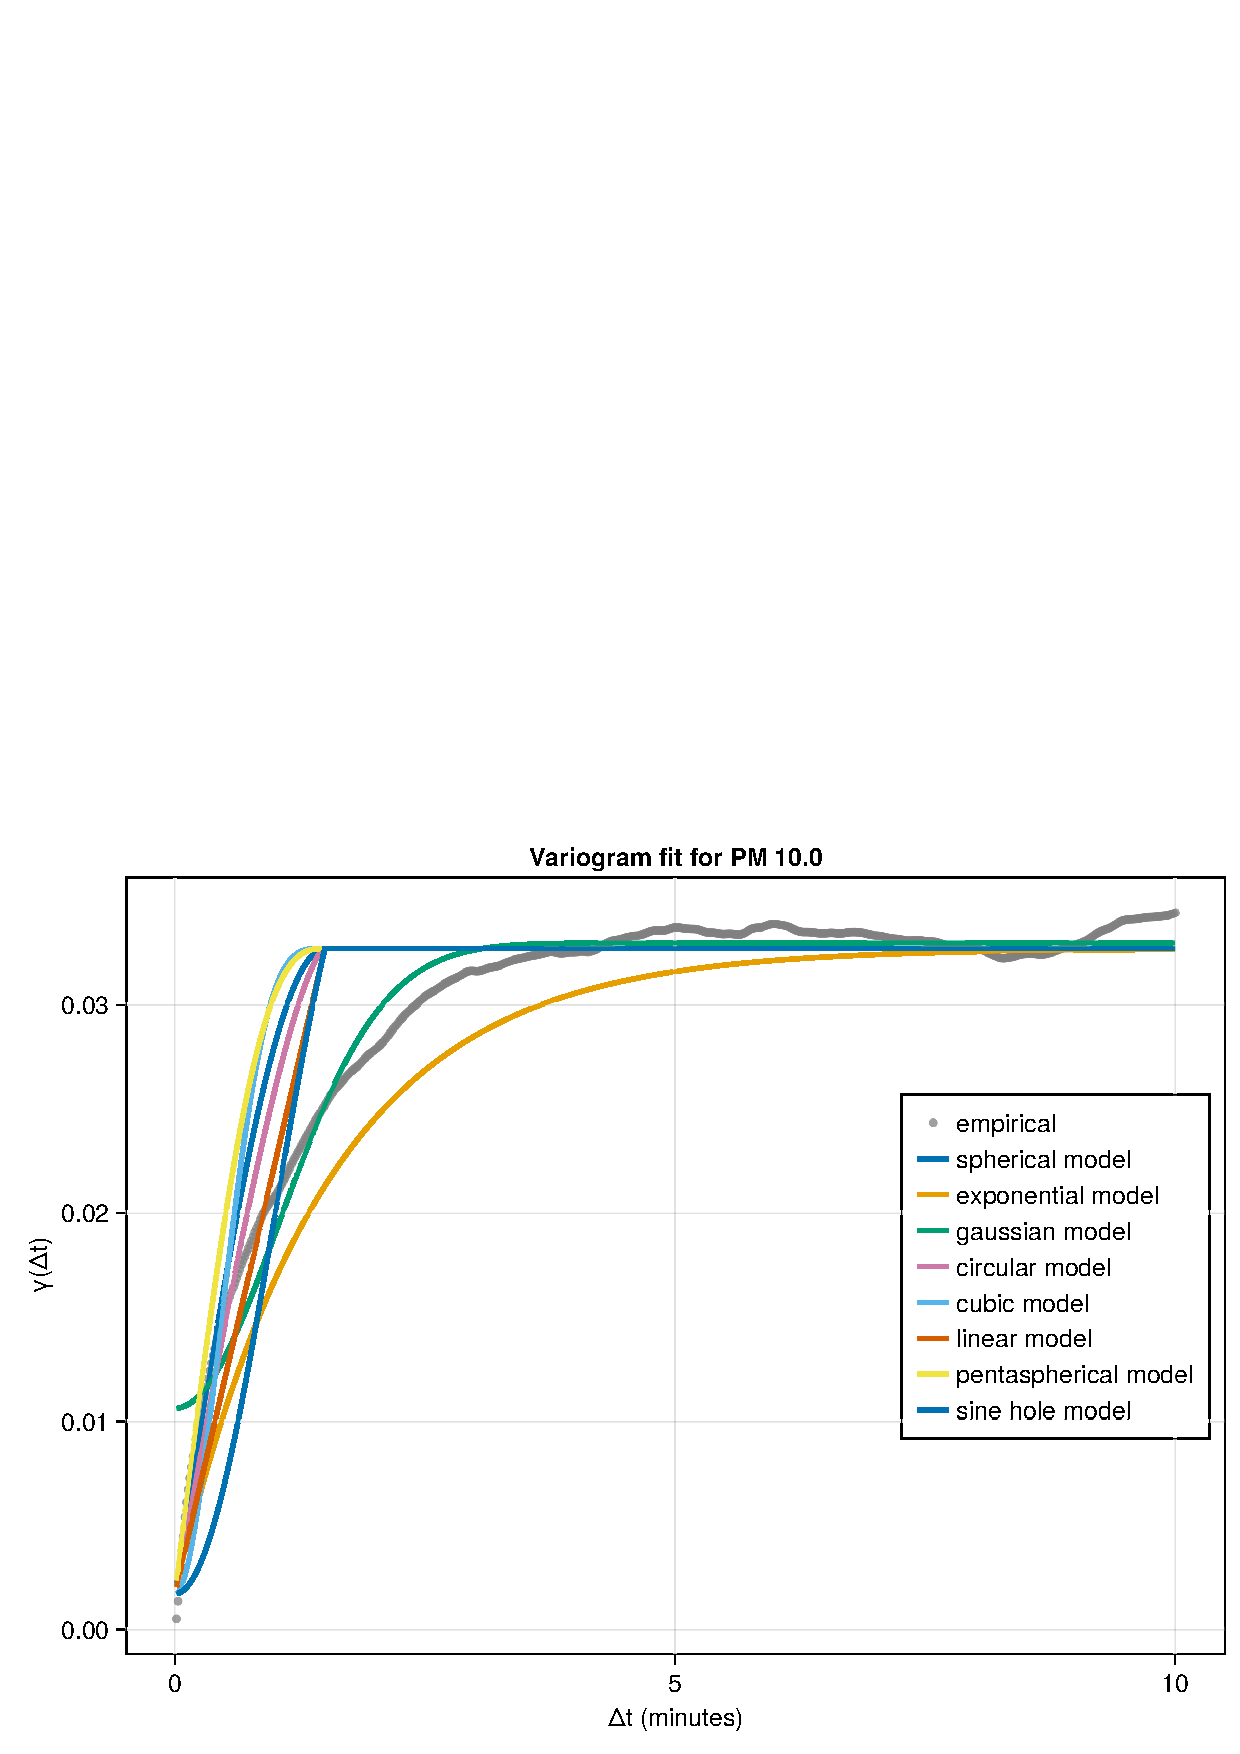
\includegraphics[width=0.85\columnwidth]{time-series/variogram/single-day/γ-PM 10.0_single-day.pdf}
  \caption{The empirical variogram and a variety of model fits obtained for the a PM $10.0$ single-day time series}
  \label{fig:pm10-variogram-fits}
\end{figure}

\subsection{Next Steps}

As of right now, I have developed an open source library to compute the temporal variogram and extract the estimated uncertainty for generic time series data. I have also developed a pipeline for the acquisition and storage of time series data in publicly available S3 buckets on the Open Storage Network. My plan now is to evaluate the uncertainty for a variety of sensors from our network for data collected across the previous 1-3 years. We will then be able to investigate how stable these uncertainty estimates are as a function of time. For example, do we see any seasonal trends during the coldest winter months and warmest summer months? Does the uncertainty appear to increase over time so that we might be able to automatically identify when a sensor should be serviced/replaced? 



\section{Physics Informed modeling techniques for Air Quality Data}


In order to provide actionable insights we must be able to effectively model the dynamics of our collected time series. In a perfect world, we would measure all relevant physical quantities such that the time evolution of local air quality at each sensor could be obtained by simulating the relevant micro-physics. However, low cost sensor networks are not equipped with all the necessary reference grade instruments needed to perform such simulations; accurate winds speed and direction sensors alone can cost hundreds to thousands of dollars and remote sensing data products are often unreliable at the ground level (i.e. in the human head space). We therefore are motivated to develop techniques to model our collected time series using only the data provided at a single node. There are many approaches to this task in the statistics and machine learning literature including statistical models like ARIMA and deep learning methods like Recurrent Neural Networks \cite{intro-to-time-series-models, time-series-rnns}. While these methods can often lead to robust short term predictions, they do not incorporate prior physics knowledge and therefore are not primed to take advantage of underlying dynamical laws. Recently two interesting physics-informed, data driven techniques have been developed for just this type of scenario. The first we shall examine is the so-called \textit{Hankel Alternative View Of Koopman} (HAVOK) framework which extends the principle of dynamic mode decomposition to nonlinear systems \cite{brunton-havok}. The second is an technique dubbed the \textit{Hamiltonian Neural Network} which extends the notion of a Neural Ordinary Differential Equation to allow a neural network to learn coordinate transformations or the original time series data which satisfy \textit{Hamiltons equations} \cite{greydanus-hnn}.

\subsection{Embedding Theorems}
\subsection{Koopman Operator Theory and Time Series Embeddings}
\subsection{A Hybrid HAVOK UDE Approach}


Motivating example: the Lorenz attractor.

\begin{figure}[h]
  \centering
  \includegraphics[width=0.85\columnwidth]{time-series/HAVOK/lorenz/havok/attractors1.png}
  \caption{Comparing the original Lorenz attractor (left) to the embedded attractor learned after performing the SVD (right). Color indicates the time along the trajectory.}
\end{figure}

\begin{figure}[h]
  \centering
  \includegraphics[width=0.85\columnwidth]{time-series/HAVOK/lorenz/havok/eigenmodes.pdf}
  \caption{Eigenmodes of the embedded attractor extracted from the SVD.}
\end{figure}

\begin{figure}[h]
  \centering
  \includegraphics[width=0.85\columnwidth]{time-series/HAVOK/lorenz/havok/heatmap.pdf}
  \caption{Heatmap of the linear Koopman operator together with the forcing activation.}
\end{figure}

\begin{figure}[h]
  \centering
  \includegraphics[width=0.85\columnwidth]{time-series/HAVOK/lorenz/havok/timeseries_reconstructed.pdf}
  \caption{The reconstructed timeseries for $v_1$ via the learned HAVOK model.}
\end{figure}

\begin{figure}[h]
  \centering
  \includegraphics[width=0.85\columnwidth]{time-series/HAVOK/lorenz/havok/scatterplot.pdf}
  \caption{A scatterplot of the resulting HAVOK fit}
\end{figure}

\begin{figure}[h]
  \centering
  \includegraphics[width=0.85\columnwidth]{time-series/HAVOK/lorenz/havok/forcing-stats.pdf}
  \caption{The statistics of the learned forcing function. The sharpness of the distribution (in comparison to a Normal distribution) indicates that the forcing is \textit{intermittent}}
\end{figure}

\begin{figure}[h]
  \centering
  \includegraphics[width=0.85\columnwidth]{time-series/HAVOK/lorenz/havok/v1_forcing_identified.pdf}
  \caption{The time series for $v_1$ marked where the forcing function is above a specified threshold.}
\end{figure}


\begin{figure}[h]
  \centering
  \includegraphics[width=0.85\columnwidth]{time-series/HAVOK/lorenz/havok/attractor_w_forcing.png}
  \caption{The embedded attractor colored by the presence of external forcing.}
\end{figure}

Now what happens if we attempt this procedure on a real, noisy dataset:



\begin{figure}[h]
  \centering
  \includegraphics[width=0.85\columnwidth]{time-series/HAVOK/sharedair/havok/attractor.png}
  \caption{The embedded attractor for PM $2.5$ time-series data.}
\end{figure}


\begin{figure}[h]
  \centering
  \includegraphics[width=0.85\columnwidth]{time-series/HAVOK/sharedair/havok/heatmap.pdf}
  \caption{Heatmap of the linear Koopman operator together with the forcing activation.}
\end{figure}


\begin{figure}[h]
  \centering
  \includegraphics[width=0.85\columnwidth]{time-series/HAVOK/sharedair/havok/timeseries_reconstructed__r-18__c-10.pdf}
  \caption{The reconstructed time-series for the first three embedding coordinates using the HAVOK fit.}
\end{figure}

\begin{figure}[h]
  \centering
  \includegraphics[width=0.85\columnwidth]{time-series/HAVOK/sharedair/havok/timeseries_reconstructed_zoomed-in.pdf}
  \caption{A zoomed in view of the same time-series reconstruction for the first $2.5$ hours showing a very decent fit. Some kind of error appears to be accumulating over time.}
\end{figure}

\begin{figure}[h]
  \centering
  \includegraphics[width=0.85\columnwidth]{time-series/HAVOK/sharedair/havok/v1_forcing_identified.pdf}
  \caption{The first embedding coordinate with forcing above a critical threshold identified.}
\end{figure}

\begin{figure}[h]
  \centering
  \includegraphics[width=0.85\columnwidth]{time-series/HAVOK/sharedair/havok/attractor_w_forcing.png}
  \caption{The original attractor now colored by external forcing above a threshold.}
\end{figure}


Now we can justify the use of a UDE approach to fit missing non-linear terms once we have a trained HAVOK model.



\subsection{Hamiltonian Neural Networks}

An alternative approach to modeling the time series is to consider a system under no external forcing. We can describe the dynamics for this system using \textit{some} set of generalized coordinates via Hamiltons equations. Now we suggest to learn an appropriate set of coordinates $(q,p)$ via an auto-encoder structure so that we can then \textit{learn} a Hamiltonian function for which these coordinates satisfy Hamilton's equations for short times. Once we have this model, we can then analyze the motion of our systems state on the Hamiltonian surface. When there is some kind of external forcing driving us away from the level sets of $H$ can we expect to see large jumps in PM concentration? Further, does the Hamiltonian function learned for a single system generalize well to multiple distributed sensors?

\begin{figure}[h]
  \centering
  \includegraphics[width=0.85\columnwidth]{time-series/HNN/hamiltonian_cn_1--2022.pdf}
\end{figure}







%% \begin{itemize}
%% \item Uncertainty Estimation Via Time Series Sampling
%% \item Types Of Uncertainty
%% \item Instrument Uncertainty
%% \item Representativeness Uncertainty
%% \item Variograms
%% \item Mutual Information
%% \item Auto-correlation
%% \item Time Series Chaos
%% \item What is Chaos?
%% \item Lyapunov Exponents
%% \item Fractal Dimension
%% \item Koopman Operator Theory
%% \item Time Series Modeling Methods
%% \item Token-Hankel Delay Embeddings
%% \item Embedding Theorems (are magic)
%% \item Determination of Optimal Lag
%% \item Determination of Intrinsic Dimension (kind of unnecessary given *large enough* embedding)
%% \item DMD and HAVOK
%% \item Hamiltonian Neural Networks
%% \item Time Series Classification
%% \item Considerations for Batching of Time Series for ML Models
%% \item K-means Clustering
%% \item Self Organizing Maps
%% \item Generative Topographic Maps
%% \item Chaos Classification via HAVOK
%% \item Symplectic and Normal Gradients for HNN
%% \item Motivating Example: Lorenz63 System
%% \item Origin of Lorenz System
%% \item Time Scale Analysis and Variography
%% \item Embedding
%% \item Modeling
%% \item Classification
%% \item Real Example 1: PM Data
%% \item Origin of Lorenz System
%% \item Time Scale Analysis and Variography
%% \item Embedding
%% \item Modeling
%% \item Classification
%% \item Real Example 2: Biometric Data
%% \item Origin of Lorenz System
%% \item Time Scale Analysis and Variography
%% \item Embedding
%% \item Modeling
%% \item Classification
%% \item Real Example 3: Stock Market Analysis
%% \item Origin of Lorenz System
%% \item Time Scale Analysis and Variography
%% \item Embedding
%% \item Modeling
%% \item Classification
%% \end{itemize}

\chapter{Chemical Reaction Mechanisms}\label{appendix:mechanisms}

\textcolor{red}{UPDATE REQUIRED!}

\chapter{Limitations and Future Work}

%% \section{Robot Team}

%% \subsection{Super Resolution}
%% Propose methods for spatial/temporal/spectral super-resolution. In particular, comment on upcoming satellite deployments like EnMAP and others which will provide hyperspectral imagery.



\chapter{Conclusions}
\textcolor{red}{\textbf{UPDATE REQUIRED!!!}}




\appendix % required only if you have appendixes

%% \chapter{Reproducible Research Techniques}
\textcolor{red}{\textbf{UPDATE REQUIRED!}}

\section{Environment Management in Julia}
\section{Version Control (git)}
\section{CI/CD with github worfklows}
discuss automated tests as well as automatic document generation here

\section{Literate Programming and Automatic Documentation with Quarto}
\section{Containerization with Docker and Docker Compose}
Discuss NodeRed, InfluxDB, Grafana, etc...



%% \chapter{Optimization Methods}

Describe standard gradient descent and it's utility for machine learning. Expand to briefly describe the extensions used in our work:
\begin{itemize}
\item Gradient Descent
\item Gradient Descent with Momentum
\item ADAM
\item BFGS
\item LBFGS
\item The method we used for the variogram method that works specifically for quadratic loss functions...
\end{itemize}

We should also comment on which particular methods are best (and when)



%% \chapter{High Performance Computing}


Provide an overview of relevant concepts in high performance computing i.e.
\begin{itemize}
\item slurm
\item multi-threading
\item parallelization (distribured computing)
\item Memory management (i.e. preallocating data containers and writing functions that mutate, not allocate)
\end{itemize}



\chapter{Chemical Reaction Mechanisms}\label{appendix:mechanisms}

\textcolor{red}{UPDATE REQUIRED!}


%% add appendices for tables of cross sections, quantum yields, and estimated photolysis rates as they may be useful for someone else...

% Begin the bibliography:

\begin{thesisbib}  % <--- THIS LINE IS REQUIRED!
  \bibliography{./references.bib}
\end{thesisbib}  % <-- THIS LINE IS REQUIRED!

\begin{biosketch}
  \textcolor{red}{\textbf{UPDATE REQUIRED!!!}}
\end{biosketch}


\begin{vita}  % <-- THIS LINE IS REQUIRED!
  \textbf{UPDATE REQUIRED!}
\end{vita}  % <-- THIS LINE IS REQUIRED!


\end{document}


